% ---- Document Class ----
\documentclass[a4paper]{llncs}

% ---- Essential Packages ----
\usepackage{amsmath}
\usepackage{amssymb}
\usepackage{graphicx}
\usepackage{hyperref}

% ---- Formatting & Layout ----
\usepackage{alltt}
\usepackage{paralist}
\usepackage{booktabs}
\usepackage{multirow}
\usepackage{colortbl}
\usepackage{arydshln}
\usepackage{wrapfig}
\usepackage[export]{adjustbox}
\usepackage{enumitem}
\usepackage{float}
\usepackage{caption}
\usepackage{subcaption}
\usepackage{tcolorbox}
\usepackage{nicefrac}

% ---- Colors ----
\usepackage[table,dvipsnames,svgnames]{xcolor}

% ---- Code Listings ----
\usepackage{listings}
\usepackage{verbatim}

% ---- Citations & References ----
\usepackage{cite}
\usepackage[capitalize]{cleveref} % Should be loaded after hyperref for best results

% ---- Math & Symbols ----
\usepackage{mathtools}
\usepackage{mathpartir}
\let\Bbbk\relax % prevent double definition with amssymb
\usepackage{wasysym}
\usepackage{pifont}
\usepackage{stmaryrd}
\usepackage{bussproofs}
\usepackage{gensymb}
\usepackage[per-mode=symbol,detect-all]{siunitx}

% ---- Other Utilities ----
\usepackage{xspace}
\usepackage{url}
\usepackage{svg}
\usepackage{ifthen}
\usepackage{etoolbox} % For patching commands
\usepackage[outline]{contour}

\usepackage{bussproofs}
\usepackage{gensymb}
\usepackage[dvipsnames]{xcolor} % adds many named colors
\usepackage[svgnames]{xcolor}

% --- LNCS + hyperref fix: correct appendix anchors, no duplicate titles ---
\usepackage{etoolbox}

% ---- TikZ Graphics ----
\usepackage{tikz}
\usetikzlibrary{shapes.geometric,positioning,arrows}

\newcommand{\cmark}{\checkmark}
%\definecolor{brightbrown}{RGB}{245,237,205}%{205,133,63}
%\colorlet{darksand}{Tan!50!black}
%\definecolor{strongyellow}{RGB}{255,220,0}
\definecolor{brightyellow}{RGB}{255,247,192}%{255,255,102}
\definecolor{lightchacki}{RGB}{245,237,205}%{235,220,187}
\usepackage{mathtools,mathpartir}
\let\Bbbk\relax   % prevent double definition
\usepackage{amssymb}
% ---- handy notation (optional) ----
\newcommand{\cfg}[3]{\langle #1,\; #2,\; #3\rangle}
\newcommand{\update}[3]{#1[#2 \mapsto #3]}
\newcommand{\step}{\mathrel{\rightarrow}}
\newcommand{\pstep}{\mathrel{\Rightarrow}}


\newcommand\blfootnote[1]{%
	\begingroup
	\renewcommand\thefootnote{}\footnote{#1}%
	\addtocounter{footnote}{-1}%
	\endgroup
}


\makeatletter
% ensure unique hyperref anchors
\renewcommand*{\theHsection}{\thesection}
\renewcommand*{\theHsubsection}{\thesubsection}
\renewcommand*{\theHsubsubsection}{\thesubsubsection}

% Patch \@sect to insert anchor *after* counter increment, without changing layout
\patchcmd{\@sect}
{\@tempskipa #5\relax}
{\refstepcounter{#1}%
	\Hy@raisedlink{\hyper@anchorstart{#1.\csname the#1\endcsname}\hyper@anchorend}%
	\@tempskipa #5\relax}
{}{}
\makeatother
% ---------------------------------------------------------------------------

% Define darkorange via RGB or HTML:
\definecolor{darkorange}{RGB}{255,140,0}

\newcommand{\xmark}{\textcolor{red}{\ding{55}}}
\usetikzlibrary{shapes.geometric,positioning,arrows} 
\definecolor{headerbg}{RGB}{220,230,241}

\newcommand{\Pre}{\mathsf{pre}}
\newcommand{\Post}{\mathsf{post}}

% ----- Macros -----

% Tool name macro (styled like typical POPL papers)
\newcommand{\toolname}{\textsc{Ser}}

\newcommand{\guy}[1]{\marginpar{\textcolor{orange}{Guy: #1}}}
\newcommand{\jules}[1]{\marginpar{\textcolor{red}{Guy: #1}}}
\newcommand{\markb}[1]{\marginpar{\textcolor{black}{Guy: #1}}}
\newcommand{\todo}[1]{\textcolor{red}{TODO: #1}}


\newcommand{\grammartag}[1]{\qquad\qquad\emph{(#1)}}


% Define macros for keywords
\newcommand{\kw}[1]{\textbf{#1}}
\newcommand{\nondet}{\kw{?}}
\newcommand{\ifkw}{\kw{if}}
\newcommand{\elsekw}{\kw{else}}
\newcommand{\whilekw}{\kw{while}}
\newcommand{\yieldkw}{\kw{yield}}
\newcommand{\requestkw}{\kw{request}}

\newcommand{\sat}{\texttt{SAT}}
\newcommand{\unsat}{\texttt{UNSAT}}

\newcommand{\Parikh}{\mathsf{Parikh}}

\newcommand{\greencmark}{\textcolor{green}{\ding{51}}}

\lstdefinelanguage{CustomPseudoCode}{
	morekeywords={request, yield, return, if, else, while, and, or},
	morecomment=[l]{//},
	morestring=[b]",
	sensitive=true
}

\lstset{
	language=CustomPseudoCode,
	basicstyle=\ttfamily\small,
	keywordstyle=\color{blue}\bfseries,
	commentstyle=\color{gray}\itshape,
	stringstyle=\color{orange},
	numbers=left,
	numberstyle=\tiny,
	stepnumber=1,
	numbersep=5pt,
	backgroundcolor=\color{white},
	frame=single,
	rulecolor=\color{black},
	tabsize=2,
	captionpos=b,
	breaklines=true,
	breakatwhitespace=false,
	showstringspaces=false,
	escapeinside={(*@}{@*)},  % used for coloring "?" below
}


% ----- Main paper -----

	\title{Deciding Serializability in Network Systems}

%\author{Anonymous}
	\author{
			Guy Amir\inst{1} \and
			Mark Barbone\inst{1} \and
			Nicolas Amat\inst{2} \and
			Jules Jacobs\inst{1,3}
		}
	

\institute{
	Cornell University, Ithaca, USA \\
	\email{ \{gda42, mlb494, jj758\}@cornell.edu} \\
	\and
	DTIS, ONERA, University of Toulouse, Toulouse, France\\
	\email{ nicolas.amat@onera.fr}\\
	\and
	Jane Street Capital, New York City, USA \\
%	\email{ \{raz.yerushalmi, david.harel\}@weizmann.ac.il}\\
}



%\settopmatter{printfolios=false,printccs=false,printacmref=false}
%\renewcommand\footnotetextcopyrightpermission[1]{} % removes footnote with DOI
% \renewcommand{\keywords}[1]{}  % removes "Additional keywords and phrases"
% \renewcommand{\acmSubmissionID}[1]{} % removes SUBMISSION ID
\let\oldmaketitle\maketitle
\renewcommand{\maketitle}{
  \oldmaketitle
  \pagestyle{plain}  % empty headers and footers on all pages
  \thispagestyle{plain}  % empty header and footer on the first page
}

% Make paragraph headings bold
%\makeatletter
%\renewcommand\paragraph{\@startsection{paragraph}{4}{\z@}%
%  {1.5ex \@plus1ex \@minus.2ex}%
%  {-1em}%
%  {\normalfont\normalsize\bfseries}}
%\makeatother

% Redefine sections to display with § symbol
\crefformat{section}{\S#2#1#3}
\Crefformat{section}{\S#2#1#3}

% Ensure subsections/subsubsections behave the same way (optional)
\crefformat{subsection}{\S#2#1#3}
\Crefformat{subsection}{\S#2#1#3}
\crefformat{subsubsection}{\S#2#1#3}
\Crefformat{subsubsection}{\S#2#1#3}

% 1) create a new length
\newlength{\subfigheight}

% 2) measure the height of (d) once the document begins
\AtBeginDocument{%
	\settoheight{\subfigheight}{%
		\includegraphics[width=0.23\textwidth]{plots/bidirectional_pruning_step_d_updated_2.pdf}%
	}%
}

% Length-related magic, to be removed for final version
%\addtolength{\oddsidemargin}{-0.2cm}
%\addtolength{\evensidemargin}{-0.2cm}
%\addtolength{\textwidth}{0.39cm}
%\addtolength{\topmargin}{-0.1cm}
%\addtolength{\textheight}{0.39cm}
%\addtolength{\intextsep}{-0.39cm}
%\addtolength{\belowcaptionskip}{-0.2cm}

% This forces \citet, \citep, etc. to behave like numeric \cite.
%\makeatletter
%\@ifpackageloaded{natbib}{}{%
%	\let\citet\cite
%	\let\citep\cite
%	\let\citealt\cite
%	\let\citealp\cite
%	\let\citeyear\relax
%	\let\citeauthor\relax
%}
%\makeatother


\begin{document}

\raggedbottom


%\begin{abstract}
%	\input{sections/0_abstract}
%\end{abstract}

\maketitle

\begin{abstract}
	\blfootnote{[*] This paper is an extended version of the paper with the same title presented at the \texttt{TACAS 2026} conference. See \url{https://etaps.org/2026/}.}
	We present the \toolname{} modeling language and toolchain for automatically verifying \textit{serializability} of concurrent programs, i.e., whether every concurrent execution of the program is equivalent to some serial execution.
	%
	\toolname{} programs are suitably restricted to make this problem decidable, while still allowing for an unbounded number of concurrent threads of execution, each potentially running for an unbounded number of steps.
	%
	Prior work has shown the theoretical decidability of this problem, but \toolname{} is the first to provide an end-to-end decision procedure and toolchain that proves serializability (generating a certificate) or non-serializability (generating a counterexample trace).
	%
	Our verifier translates network system programs into Petri nets, and curtails the search space by employing various optimizations, such as Petri net slicing, semilinear-set compression, and Presburger-formula manipulation.
	%
	We extensively evaluate our toolchain and demonstrate that, despite the theoretical hardness of the problem, it can successfully run on various real-world programs, including stateful firewalls, BGP routers, online shopping backends, and more.
\end{abstract}

% \keywords{programming languages, static analysis, verification}


\section{Introduction}
\label{sec:introduction}

\todo{Introduction goes here.}

\todo{We motivate the problem of deciding serializability in programmable networks.}

\todo{We talk about some related work if relevant.}

\todo{We show that it's interesting with an example.}

\todo{We describe our main results.}

\paragraph{Contributions:}
\begin{itemize}
    \item Novel notion of serializability (``atomicity'') applicable to network systems
    \item Decidability results (1 main theorem: \textbf{automatically proving unbounded serializability}, 2 extra theorems: ser=ser decidable, ser=int undecidable)
    \item Implementation of decision procedure
    \item Advances in semilinear sets, Petri net reachability heuristics that makes the decision procedure work
\end{itemize}
\section{Problem Definition}
\label{sec:problemDefinition}

\begin{figure}[t]
    \begin{align*}
    e ::= &&&\\
       | & \; 0 \mid 1 \mid 2 \mid \ldots                                && \text{(numeric constants)} \\
       | & \; \nondet                                 && \text{(nondeterministic value: 0 or 1)}\\
       | & \; x := e                            && \text{(write to local variable / packet field)} \\
       | & \; x                                 && \text{(read from local variable / packet field)} \\
       | & \; X := e                            && \text{(write to global variable / switch variable)} \\
       | & \; X                                 && \text{(read from global variable / switch variable)} \\
       | & \; e_1 == e_2                        && \text{(equality test)} \\
       | & \; e_1 ; e_2                         && \text{(sequencing)} \\
       | & \; \ifkw(e_1)\{e_2\}\elsekw\{e_3\} && \text{(conditional)} \\
       | & \; \whilekw(e_1)\{e_2\}              && \text{(loop)} \\
       | & \; \yieldkw                      && \text{(yields to scheduler)}
    \end{align*}
    \caption{Syntax of expressions}
    \label{fig:syntax}
\end{figure}
    
A Network System $\mathcal{N}$ is a tuple $(G, L, \mathit{Req}, \mathit{Res}, g_0, \delta, \mathit{req}, \mathit{resp})$ where:
\begin{itemize}
\item $G$ is a set of global states representing switch state
\item $L$ is a set of local states representing packet contents
\item $\mathit{Req}$ is a set of request events
\item $\mathit{Res}$ is a set of response events
\item $g_0 \in G$ is the initial global state
\item $\mathit{req} \subseteq \mathit{Req} \times L$ is a request transition relation, which describes which requests turn into which packets
\item $\mathit{resp} \subseteq L \times \mathit{Res}$ is a response transition relation, which describes which packets turn into which responses
\item $\delta \subseteq (G \times L) \times (G \times L)$ is a transition relation for packet processing, which describes an atomic step of packet processing that may change the global state.
\end{itemize}

\begin{figure}[t]
    \centering
    \renewcommand{\arraystretch}{1.6}
    \[
    \begin{array}{c}
    \textbf{States and Transitions:}
    \\
    \quad
    \text{A (global) \emph{network state} is a triple }(g,\mathcal{P},M)\text{ where:}
    \\
    \quad
    g \in G \text{ is the current global switch state,}
    \\
    \quad
    \mathcal{P} \in \text{Multiset}(L \times \mathit{Req}) \text{ is a multiset of in-flight packets,}
    \\
    \quad
    M \in \text{Multiset}(\mathit{Req} \times \mathit{Res}) \text{ is a multiset of request--response pairs already completed.}
    \end{array}
    \]

    \[
    \begin{array}{c}
    \textbf{Initial state:}
    \\
    \quad (g_0,\,\varnothing,\,\varnothing)
    \end{array}
    \]

    \[
    \begin{array}{c}
    \textbf{Transition rules:}
    \\[1em]
    \text{(New Request)}\quad\infer{
    (r,\ell)\,\in\,\mathit{req}
    }
    {(g,\;\mathcal{P},\;M) \;\longrightarrow\; (g,\;\mathcal{P} \uplus \{(\ell,r)\},\;M)}
    \\[2em]
    \text{(Packet Step)}\quad\infer{
    ((g,\ell),\,(g',\ell')) \,\in\, \delta
    }
    {(g,\;\mathcal{P} \uplus \{(\ell,r)\},\;M) \;\longrightarrow\; (g',\;\mathcal{P} \uplus \{(\ell',r)\},\;M)}
    \\[2em]
    \text{(Response)}\quad\infer{
    (\ell,s)\,\in\,\mathit{resp}
    }
    {(g,\;\mathcal{P} \uplus \{(\ell,r)\},\;M) \;\longrightarrow\; (g,\;\mathcal{P},\;M \uplus \{(r,s)\})}
    \end{array}
    \]

    \[
    \begin{array}{c}
    \textbf{Complete runs:}
    \\
    \quad (g_0,\,\varnothing,\,\varnothing) \;\longrightarrow\; (g_1,\,\mathcal{P}_1,\,M_1) \;\longrightarrow\; \cdots \;\longrightarrow\; (g_n,\,\mathcal{P}_{n-1},\,M_{n-1}) \;\longrightarrow\; (g_n,\,\varnothing,\,M_n)
    \\[1em]
    \textbf{Interleaved run: } \text{the } \mathcal{P}_i \text{ can have more than one packet, and } \mathcal{P}_n = \varnothing \\
    \textbf{Serial run: } \text{ each } \mathcal{P}_i \text{ has at most one packet, and } \mathcal{P}_n = \varnothing\\
    \text{Int}(\mathcal{N}) = \{ M \in \text{Multiset}(\mathit{Req} \times \mathit{Res}) \mid \exists \text{ interleaved run } (g_0,\,\varnothing,\,\varnothing) \;\longrightarrow^*\; (g_n,\,\varnothing,\,M) \}\\
    \text{Ser}(\mathcal{N}) = \{ M \in \text{Multiset}(\mathit{Req} \times \mathit{Res}) \mid \exists \text{ serial run } (g_0,\,\varnothing,\,\varnothing) \;\longrightarrow^*\; (g_n,\,\varnothing,\,M) \}\\
    \end{array}
    \]

    \caption{State-transition rules for executions of
    \(\mathcal{N} = (G, L, \mathit{Req}, \mathit{Res}, g_0, \delta, \mathit{req}, \mathit{resp})\).
    A transition \(\longrightarrow\) modifies the triple \((g,\mathcal{P},M)\) by either (1) introducing a new request, (2) processing a packet step via \(\delta\), or (3) consuming a packet to produce its response.  When no more steps are possible, the result set \(M\) is the final multiset of request--response pairs that arose during the run.
    Runs are called \emph{serial} if there is at most one packet in flight at any time, whereas \emph{interleaved} runs may have multiple packets in flight at once.}
    \label{fig:network-transitions}
\end{figure}

\begin{definition}[Interleaved executions \(\mathrm{Int}(\mathcal{N})\)]
    Let \(\mathcal{N} = (G, L, \mathit{Req}, \mathit{Res}, g_0, \delta, \mathit{req}, \mathit{resp})\).
    An \emph{interleaved execution} begins in global state \(g = g_0\) with no packets in flight.
    At any point, one may:
    \begin{itemize}
        \item introduce a new request \(r \in \mathit{Req}\), producing an in-flight packet \(\ell \in L\) if \((r,\ell) \in \mathit{req}\);
        \item take an in-flight packet \(\ell\) and transition \(\ell \mapsto \ell'\) and \(g \mapsto g'\) if \(((g,\ell),(g',\ell'))\in\delta\);
        \item consume an in-flight packet \(\ell\) to produce a response \(s\) if \((\ell,s)\in \mathit{resp}\).
    \end{itemize}
    Each request \(r\) must eventually yield exactly one corresponding response \(s\) in a valid execution.
    The set of all finite multisets of \((r,s)\) pairs realizable by such interleavings is:
    \[
        \mathrm{Int}(\mathcal{N})
        \;=\;
        \bigl\{
        M \;\in\; \text{Multiset}(\mathit{Req}\times \mathit{Res})
        \;\mid\;
        M \text{ is realized by some interleaved run of }\mathcal{N}
        \bigr\}.
    \]
\end{definition}

\begin{definition}[Serial executions \(\mathrm{Ser}(\mathcal{N})\)]
In a \emph{serial} execution, requests are processed one at a time:
\begin{enumerate}
    \item Start in \(\,g_0\).
    \item Take a single request \(r\in \mathit{Req}\), convert it to a packet, process that packet until a response \(s\in \mathit{Res}\) is produced.
    \item Update the global state accordingly and repeat with the next request.
\end{enumerate}
No two requests overlap in processing.
The set of all finite multisets of \((r,s)\) pairs realizable by such one-at-a-time runs is:
\[
    \mathrm{Ser}(\mathcal{N})
    \;=\;
    \bigl\{
    M \;\in\; \text{Multiset}(\mathit{Req}\times \mathit{Res})
    \;\mid\;
    M \text{ is realized by some serial run of }\mathcal{N}
    \bigr\}.
\]
\end{definition}

\begin{theorem}[Serializability]
\label{thm:int-eq-ser}
Whether
\(
    \mathrm{Int}(\mathcal{N}) \;=\; \mathrm{Ser}(\mathcal{N})
\)
holds is decidable.
\end{theorem}

\begin{theorem}[Serial Equivalence]
\label{thm:ser-eq-ser}
Whether
\(
    \mathrm{Ser}(\mathcal{N}) \;=\; \mathrm{Ser}(\mathcal{N})
\)
holds is decidable.
\end{theorem}

\begin{theorem}[Interleaved Equivalence]
\label{thm:int-eq-int}
Whether
\(
    \mathrm{Int}(\mathcal{N}) \;=\; \mathrm{Int}(\mathcal{N})
\)
holds is undecidable.
\end{theorem}
\section{Formal results}
\label{sec:formal-results}



\section{Implementation}
\label{sec:implementation}
\begin{wraptable}[11]{r}{0.32\textwidth}
	\vspace{-1.5em} 
	\centering
	\begin{tabular}{@{} l S[table-format=5.0] @{}}
		\toprule
		\textbf{Module}                & {\textbf{LoC}} \\
		\midrule
		Input \& Parsing               &  1723          \\
		Model Construction             &  5561          \\
		Petri--Net Conversion           &   843          \\
		Reachability          &  2628          \\
		Proof Checking                 &  3240          \\
		Utilities                      &  2160          \\
		Testing \& Evaluation          &  2118          \\
		\midrule
		\textbf{Total}                 & \textbf{18273} \\
		\bottomrule
	\end{tabular}
	\caption{Lines of Code}
	\label{tab:loc_summary2}
\end{wraptable}
%\vspace{-1.5\baselineskip} % nudge following text up a bit
We implemented our approach in \toolname{}~\cite{ArtifactRepository}, a publicly available toolchain consisting of over $18{,}200$ LoC written mostly in \texttt{Rust} (see Table~\ref{tab:loc_summary2}).
%
%We next elaborate on the architecture of our tool and the various optimizations we added to allow it to run efficiently.
%
%For the underlying Petri Net model checker, we use SMPT~\cite{AmDa23} which supports \textit{unbounded} reachability queries (see Appendix~\ref{appendix:smpt}).
%, and which uses Z3 as an underlying SMT solver~\cite{DeBj08}. 
%and which we extended to support our setting (for example, we needed to extend the solver to support proof generation). 
%
%We note that other off-the-shelf solvers can be used as well.

%The implementation..

%\begin{enumerate}
%	\item The extra things we did to make the thing actually run
%	\item Code architecture
%	\item Optimizations
%\end{enumerate}

%\newpage
\subsection{Code Architecture}

%\begin{tabular}{|l|r|}
%	\hline
%	\textbf{Module} & \textbf{LoC} \\
%	\hline
%	Input \& Parsing                             & 1723  \\
%	\hline
%	Model Construction                           & 5561  \\
%	\hline
%	Petri-Net Conversion                         & 843   \\
%	\hline
%	Reachability Checking                        & 2628  \\
%	\hline
%	Proof Checking                               & 3240  \\
%	\hline
%	Utilities                                       & 2160  \\
%	\hline
%	Testing \& Evaluation               & 2118  \\
%	\hline
%	\textbf{Total}                               & \textbf{18273} \\
%	\hline
%\end{tabular}


%
%\begin{table}[ht]
%	\centering
%	\label{tab:loc_summary}
%	\begin{tabular}{@{} l S[table-format=5.0] @{}}
%		\toprule
%		\textbf{Module}                & {\textbf{LoC}} \\
%		\midrule
%		Input \& Parsing               &  1723          \\
%		Model Construction             &  5561          \\
%		Petri–Net Conversion           &   843          \\
%		Reachability Checking          &  2628          \\
%		Proof Checking                 &  3240          \\
%		Utilities                      &  2160          \\
%		Testing \& Evaluation          &  2118          \\
%		\midrule
%		\textbf{Total}                 & \textbf{18273}          \\
%		\bottomrule
%	\end{tabular}
%	\caption{Lines of Code by Module}
%\end{table}
%

% Then, where you want the table wrapped to the right:
%
% this table summarizes the values without whitespaces/comments and without the code for SMPT (or the wrapper) or the carfo and toml files
%
%\begin{wraptable}[8]{r}{0.32\textwidth}
%	\centering
%	\begin{tabular}{@{} l S[table-format=5.0] @{}}
%		\toprule
%		\textbf{Module}                & {\textbf{LoC}} \\
%		\midrule
%		Input \& Parsing               &  1723          \\
%		Model Construction             &  5561          \\
%		Petri–Net Conversion           &   843          \\
%		Reachability          &  2628          \\
%		Proof Checking                 &  3240          \\
%		Utilities                      &  2160          \\
%		Testing \& Evaluation          &  2118          \\
%		\midrule
%		\textbf{Total}                 & \textbf{18273} \\
%		\bottomrule
%	\end{tabular}
%	\caption{Lines of Code (LoC)}
%	\label{tab:loc_summary2}
%\end{wraptable}
%
%\noindent
%
\toolname{} implements an end-to-end serializability checker for a given input program. If the program is serializable, we return a proof thereof; otherwise, if it is not serializable, a counterexample is given to the user for an interleaving that can result in request/response pairs that are unattainable in any serial execution.
%
Our workflow translates the decidability problem to an equivalent Petri net reachability question (for an unbounded number of tokens), in which (i) the Petri net represents all possible interleavings of the program; and (ii) the reachability query represents a semilinear set (equivalently, a Presburger arithmetic encoding) of all request/response pairs that \textit{cannot} be obtained by any serial execution.
%
As Petri net reachability is \texttt{Ackermann}-complete~\cite{CzWo22}, we added various optimizations to expedite the search process, both at the PN level and the property-encoding level.
%
The pipeline of \toolname{} is depicted in Fig.~\ref{fig:full_program_flow}, and includes:
 

\begin{enumerate}
	\item \textbf{Input \& parsing.} 
	Our framework receives either a \texttt{SER} program with the syntax described in~\Cref{sec:problem-definition}; or a \texttt{JSON} file directly encoding a network system. In the case of the former, an additional step takes place, parsing the input %(using the \texttt{parser.rs} module) 
	to an expression tree that is translated to the equivalent NS.
%	, represented as a struct in the \texttt{ns.rs} module. 
	
	\item \textbf{Petri net conversion.} The NS is then translated into a Petri net 
%	(see the \texttt{petri.rs} module) 
which represents all possible interleavings. 
%	.as depicted, for example, in subsec.~\ref{subsec:ns-not-serializable}.
%	Each place represents a state (either global or local) or a response. Each token represents a single in-flight request or a terminated response. 
The PN is encoded in the de facto standard \texttt{NET} format, to support off-the-shelf PN model checkers. 
	
	\item \textbf{Semilinear conversion.} 
%	This includes a set of modules (\texttt{kleene.rs}, \texttt{semilinear.rs}, and \texttt{presburger.rs}) which 
We generate a semilinear set encoding all non-serializable outputs, via translation of the serialized NFA (e.g., Fig.~\ref{fig:code2ExampleNFA}) to a regex, which is then projected (via the Parikh image) and complemented. 
%	This conversion is done by the following pipeline: (1) the NS is translated to an NFA encoding all possible request/response pairs of the input program; (2) This NFA is translated to a regex (via Kleene's Theorem) and then projected (via the Parikh Image) to a semilinear set. The (finite) encoding of the semilinear set symbolically represents all outputs attained via serializable executions of the program, running for an unbounded number of steps; (3) finally, we complement the semilinear set to encode all outputs unattainable via serial executions. 
	At the end of the pipeline, an \texttt{XML}-formatted output encodes a reachability query that encapsulates constraints over the PN token count.
	
	
	\item \textbf{Reachability engine.} The PN and the reachability query are fed to a  PN model checker, which combines \textit{bounded model checking} (BMC)~\cite{BiCiClZh99} in search of a counterexample; and \textit{state equation reasoning}~\cite{Mu77} in order to prove non-reachability. 
%	This engine is implemented in the \texttt{reachability.rs} and \texttt{reachability\_with\_proofs.rs}  modules.
	%
	In order to expedite the search, ``large'' (PN, query) pairs are replaced with multiple sliced PNs (generated by the reachability engine), each coupled with a sub-query encoding a separate disjunct. 
%	of the original query.
%	We iteratively solve the 
The disjuncts are solved on the fly, until reaching \texttt{SAT}, in which case, we have a counterexample; otherwise, if all disjuncts are \texttt{UNSAT}, we render the original program as serializable.
	
	
	\item \textbf{Proof \& certification.} 
	If \texttt{SAT}, we reconstruct and validate an NS-level counterexample. Otherwise, if all disjuncts are \texttt{UNSAT}, we extract per-disjunct proofs and ``stitch'' these to a single inductive serializability certificate, which we then project to the NS and validate (i) initiation, (ii) inductiveness, and (iii) query refutation.
	%
%	If the query is \texttt{SAT}, we reconstruct a non-serializable NS-level execution and validate its correctness. Otherwise, if all disjuncts are \texttt{UNSAT}, our proof module extracts a separate proof for each disjunct. We subsequently ``stitch'' these proofs to a single inductive invariant, and project it to the NS-level, representing a full inductive proof certificate for serializability. Our checker also validates that the inductive invariant is correct, i.e., (i) includes the initial state; (ii) is inductive with regard to the transitions; and (iii) implies that the reachability query is \texttt{UNSAT}.
	%, and hence, implying serializability. 
	
	
	\item \textbf{Instrumentation \& logging.} Throughout the pipeline, we record various intermediate representations and performance metrics.  
%	input size and performance metrics (number of places, transitions, constraint complexity, timings) 
%
%The logger outputs 
%We generate \texttt{CSV} and \texttt{JSON} logs along with
% analysis. 
	%
%	We also assemble 
%an \texttt{HTML} report embedding the original net, symbolic constraints, reachability results, proofs, etc.
%	\item \textbf{Debug Report Generation.} Finally, a human-readable \texttt{HTML} report is assembled: it embeds the original net, symbolic constraints, reachability results, proof outlines, and profiling graphs. This interactive report allows users to drill down into each transition firing, constraint check, and proof obligation.
	
%	\item \textbf{Output Delivery.} The crate exposes a simple CLI and library API. Users obtain either a Boolean reachability verdict (with optional certificate), raw log files, or a full HTML debug report, depending on invocation flags.
	
%	\item \textbf{Optimizations.} As formalized in the previous section, we implement multiple optimizations throughout the process.
%	, both for representing the semilinear sets succinctly and for pruning the Petri Nets. These optimizations significantly reduce the search space and expedite the model-checking process.
\end{enumerate}



%\noindent
%This linear pipeline - \emph{parse} -> \emph{model} -> \emph{normalize} -> \emph{analyze} -> \emph{prove} -> \emph{report} --- ensures a clear separation of concerns, easy extensibility (e.g., swapping backends), and comprehensive traceability from input to certified result.```


\begin{figure}[!htbp]
	\centering
	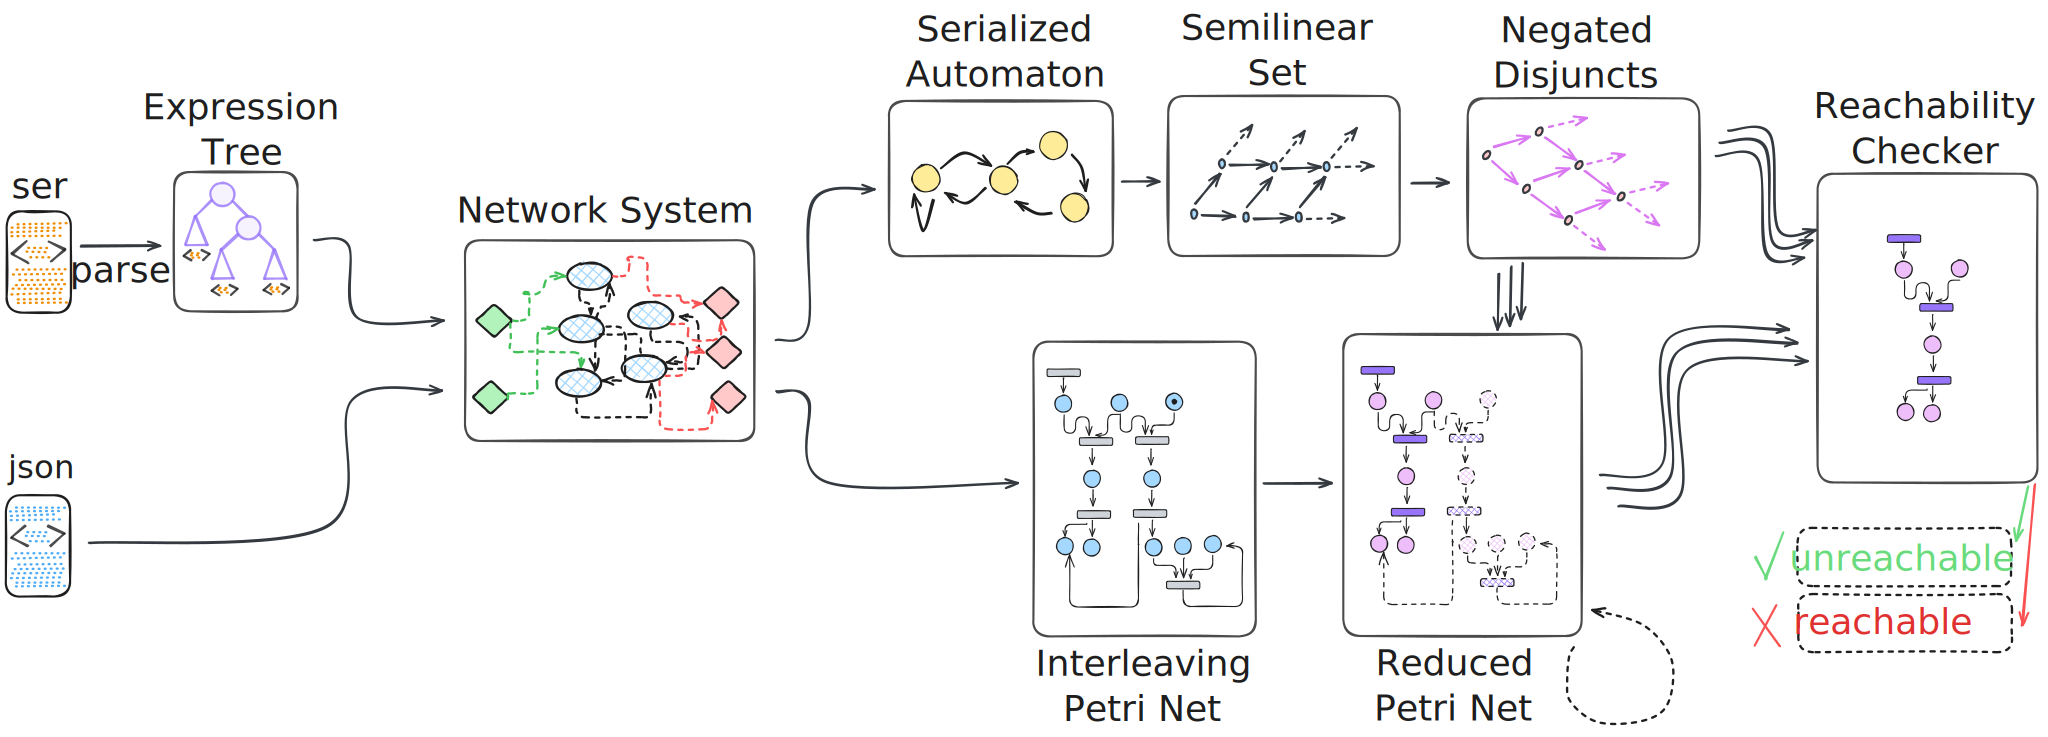
\includegraphics[width=1.0\textwidth]{plots/full_program_flow.pdf}
	\caption{Full program flow 
%		If the target set is unreachable --- a serializability proof is produced; otherwise, if it is reachable --- a counterexample trace is generated.
	(simplified, without backward arrows 
%	translating invariants (if serializable) or counterexample traces (if non-serializable) back 
	to the NS level).}
	\label{fig:full_program_flow}
\end{figure}


%\subsection{Optimizations}

%\paragraph{Bidirectional Pruning of the Petri Net}
%Before any heavy symbolic reasoning takes place, we apply bidirectional pruning on the underlying PN.  In the forward pass, we traverse from the initial marking to identify all places and transitions that could ever fire; in the backward pass, we traverse backward from any place that can influence a target constraint, and identify transitions and places that cannot contribute to reaching it.  By iteratively repeating forward passes and backward passes until convergence, we remove every component of the net that cannot both originate and contribute to the reachable target set.  This dramatically shrinks the net in practice, often converting an intractably large model into one small enough for exhaustive analysis.
%%
%We depict this in Fig.~\ref{fig:bidirectional_pruning}, and give a formal proof of correctness in Appendix~\ref{appendix:BidirectionalProof}.

%\paragraph{Redundant‐Constraint Elimination}
%When manipulating Presburger sets or their semilinear representations, it is common for some inequalities or disjuncts to add no new coverage beyond what other constraints already guarantee.  The redundant‐constraint elimination pass inspects each linear inequality and each disjunct in a disjunctive normal form, testing whether it is implied by the rest.  Any constraint or disjunct found redundant is dropped, ensuring that subsequent intersection, union, and projection operations work on the smallest necessary formula.  This streamlines the logic formula and prevents exponential blow‐up of case distinctions during solver invocations.
%
%Every time you build or star a semilinear set, you prune out any “period” vectors that are rendered useless by earlier steps:. nce you’ve accumulated a bunch of LinearSet components, you try to merge any that mathematically subsume one another:

%\paragraph{Generating Fewer Constraints}
%During set‐construction--- especially when introducing new existentially‐quantified variables or combining transition effects, we selectively avoid generating any marking that would strictly dominate an already‐seen solution.  In effect, whenever a candidate disjunct would yield a superset of an existing one, it is skipped entirely.  This ``generate‐less” heuristic stops the proliferation of large, overlapping regions in the semilinear description, trading off completeness of intermediate case‐enumeration for concise final representations.  In benchmarks with large state‐spaces, it can reduce the number of intermediate branches by orders of magnitude.

%in both the Regex and SemilinearSet Kleene-algebra instances. Concretely, instead of always building the full new structure and pruning it later, operations like union (plus) and concatenation (times) do a quick check for trivial cases and drop “zero” or “one” elements on the spo

%\paragraph{Executing Kleene Elimination in a Strategic Order:}
%When converting an NFA to a single regex, we pick the next state to eliminate by heuristically choosing the  state with the fewest incoming and outgoing edges.
%This optimization allows circumventing 
%overblown expressions resulting in naive translations, especially with regard to  Kleene closures (the “\(\mathsf{*}\)” operator).  Instead, we analyze the structure of sub-expressions under the various operators --- estimating their branching factor, and reorder them so that simpler, low‐branching components are expanded first.  This adaptive ordering often leads to early detection of fixed points or dead‐ends, preventing the combinatorial explosion that arises when complex loops are expanded prematurely.  




\subsection{Benchmark Overview} 
\label{subsec:benchmarks}
To the best of our knowledge, ours is the first and only tool to: (i) statically check serializability on \textit{unbounded} programs; and (ii) \textit{prove serializability holds}.
%
Thus, due to a lack of standard benchmarks for evaluating serializability, we 
assembled a suite of dozens of benchmarks (as part of our accompanying artifact~\cite{ArtifactRepository}).
These include both serializable and non-serializable instances encoded in both \texttt{SER} and \texttt{JSON} formats, and covering a broad range of features, including arithmetic, locks, loops, non-determinism, and more (see an overview of all our benchmarks in Table~\ref{tab:benchmarks-all} of Appendix~\ref{appendix:full_results}).
%
We note that although the benchmarks themselves are not the main part of the paper, we believe that they have merit on their own, due to their relevance to various real-world systems of interest.
%
Specifically, we wish to note our suite of benchmarks encoding \textit{network \& system protocols} (see Table~\ref{tab:networking-benchmarks}), which include stateful firewalls, BGP routing programs, network monitors, and more --- 
%highlighting the serializability challenges inherent in real-world distributed programs.
%
%Here, we were motivated by 
as motivated by real-world concurrency problems in this domain. One such example is our \textit{routing-cycle benchmark} in software-defined networks (motivated by~\cite{NaGhSa24}). Another real-world example is our \textit{snapshot isolation benchmark} (see Appendix~\ref{appendix:tour}), that was motivated by a real database bug, namely, duplicate-key errors~\cite{cockroach-issue-14099} in the popular \texttt{CockroachDB} system~\cite{cockroachdb-si-docs}.
%
In both cases and others, the non-serializable behavior was automatically identified by our toolchain.
%
%Our benchmarks include both serializable and non-serializable instances, and their features and categorization appears in Table~\ref{tab:benchmarks-all}. 



%As there are no standard benchmarks for evaluating serializability, we wrote dozens of programs in our abstract NS language. These benchmarks span a wide range of complexity --- covering branching, looping constructs, arithmetic, non-deterministic choice, and multi-request workflows that manipulate both shared (global) variables and per-request (local) state. 
%
%We include both serializable and non-serializable instances and summarize the benchmarks' features and categorizations in Table~\ref{tab:benchmarks-all}. 
%
%In particular, our most sophisticated examples are drawn from realistic networking and system-protocol scenarios, including stateful firewalls, BGP routing, network monitoring, and more --- highlighting the serializability challenges inherent in real-world distributed programs.
%
%As there are no official benchmarks for evaluating serializability, we hand-coded dozes of programs in our abstract network-system language.
%%
%The benchmarks vary in the complexity, and have multiple features: branching, loops, arithmetic, non-determinism, and multiple requests and responses, operating on both shared (global) variables and per-request (local) variables.
%%
%The benchmarks include both serializable and non-serializable instances, as we summarize in Table.~\ref{tab:benchmarks-all}, based on a category and feature-wise breakdown.
%%
%Especially, we wish to note the final category of complex examples as motivated by real-world systems and networking programs.
%%
%These include a stateful firewall, BGP routing, network monitoring and additional examples.
%
%\begin{itemize}
%		
%	\item \todo{update benchmark overview and category names}
%	\item \textbf{Core expressions \& multi request workflows}: Benchmarks testing arithmetic, boolean, and simple control expression.
%	\item \textbf{Fred (mixed arithmetic)}: Mixed control and arithmetic transformations (Fred series).
%	\item \textbf{Stop (circular-increment) series}: Circular increment loops and variants.
%	\item \textbf{Concurrency \& locking loops}: Concurrent looping patterns with locking and tricky interactions.
%	\item \textbf{Non-deterministic choice \& randomness}: Random choice and non-deterministic branching benchmarks.
%	\item \textbf{Networking \& system protocols}: Networking protocols and system-level monitoring.
%	\item \textbf{JSON state-machine examples}: Example JSON-encoded state machine workflows.
%\end{itemize}
%
%
%
%The benchmarks differ in their complexity and in the various features pertaining to them --- branching, loops, randomness, multiple requests, etc. 
%



\newpage
\section{Evaluation}
\label{sec:evaluation}

%\begin{enumerate}
%    \item Benchmarks (describe our benchmarks)
%    \item Results (total time, split out SMPT time from our rust code time)
%    \item Analysis of optimizations (how much time they save, petri net sizes, semilinear set sizes)
%    \item Limitations (examples we cannot solve, future work that would help)
%\end{enumerate}


\noindent
\textbf{Experimental Setup.}
All experiments ran on a Lenovo ThinkPad P16s, with 16 AMD cores and 64 GB of RAM, running on a Linux Ubuntu 24.04.2 operating system.
%
%We plan on making all our code, benchmarks raw results publicly available with the final version of this paper.
%
Our code, benchmarks, and full experimental results are publicly available~\cite{ArtifactRepository}.
%
%All experiments were run with a \texttt{TIMEOUT} value of $150$ seconds.
 



\subsection{Runtime Results}
We ran \toolname{} on all 47 benchmarks, out of which 27 are serializable, and the remaining 20 are non-serializable. 
For each benchmark, we measured the time for deciding the reachability query, as well as the overall time, including validation of the invariant proof (if serializable) or of the counterexample (if not serializable). These experiments ran in parallel on $16$ cores with all four optimizations and a \texttt{TIMEOUT} threshold of $500$ seconds.
%
Within the time limit, \toolname{} solved 26 of the 27 serializable benchmarks and 19 of the 20 non-serializable benchmarks (see summary in Table~\ref{tab:stats-summary} and the full results in Table~\ref{tab:benchmarks-all} of the appendix).
%
% As can be seen by our results (summarized in Table~\ref{tab:benchmarks-all}), withing this time limit, our tool fully solved 26/27 serializable benchmarks 
%and 19/20 non serializable benchmarks. 
%
The \textit{median} total runtime was $2{,}080$ ms across all benchmarks, and $2{,}238.50$ ms ($830$ ms) when focusing on solely serializable (non-serializable) benchmarks.
%, as reported in Table~\ref{tab:stats-summary}.
%
The \textit{average} total runtime was $52{,}857.55$ ms across all benchmarks, and $25{,}530.69$ ms ($42{,}980.47$ ms) when focusing on solely serializable (non-serializable) benchmarks.
%
We also observe a clear runtime split based on serializability: 
%For serializable benchmarks, certificate validation takes much longer than proof generation. 
among non-serializable benchmarks, counterexample generation is much longer than validation, and dominates the runtime; whereas the opposite holds in non-serializable benchmarks. This is not surprising, as validating a given counterexample only requires a polynomial-time simulation of the network to confirm its feasibility.
%
%We also note that when analyzing the benchmarks based on their serializability, there is a clear difference in their average runtime --- while in the serializable benchmarks the validation of the certificate takes significantly longer than generating the certificate (i.e., the proof) --- in the non serializable benchmarks this trend is reversed, with the overall time being dominated by the generation of the counterexample. This of course is not surprising, as counterexample generation can be done in polynomial time by emulating our network system and checking that the final counterexample can indeed be attained.
%
%We report the full results in Table~\ref{tab:stats-summary} and Table~\ref{tab:benchmarks-all}.
%, and elaborate on the per-benchmark results in Table~\ref{tab:benchmarks-all}.


%\begin{table}[!htbp]
%	\centering
%	% Load the tabular from the external file:
%	\begin{table}[H]
	\centering
	\begin{tabular}{l r r r r}
		\toprule
		& \multicolumn{2}{c}{Average time (ms)} 
		& \multicolumn{2}{c}{Median time (ms)} \\
		\cmidrule(lr){2-3} \cmidrule(lr){4-5}
		Category
		& \shortstack{certificate\\generation}
		& total
		& \shortstack{certificate\\generation}
		& total \\
		\midrule
		Serializable      &   2{,}273 &  25{,}531 &  1{,}178 &  2{,}238 \\
		Not serializable  &  42{,}076 &  42{,}980 &   773 &   830 \\
		All               &  39{,}613 &  52{,}858 &   797 &  2{,}080 \\
		\bottomrule
	\end{tabular}
\end{table}

%	\caption{Average and median runtime. Values are rounded to the nearest integer, to reduce clutter. The \textit{total} column also includes the time for validation.}
%	\label{tab:stats-summary}
%\end{table}



%\begin{table}[H]
%	\centering
%	% Load the tabular from the external file:
%	\begin{table}[H]
	\centering
	\begin{tabular}{lrrrrrr}
		\toprule
		& \multicolumn{3}{c}{Average time (ms)} & \multicolumn{3}{c}{Median time (ms)} \\
		\cmidrule(lr){2-4} \cmidrule(lr){5-7}
		Category
		& \shortstack{certificate\\generation}
		& \shortstack{certificate\\validation}
		& total
		& \shortstack{certificate\\generation}
		& \shortstack{certificate\\validation}
		& total \\
		\midrule
		Serializable      &   2273 &  23257 &  25531 &  1178 &  1300 &  2238 \\
		Not serializable  &  42076 &    905 &  42980 &   773 &    78 &   830 \\
		All               &  39613 &  13244 &  52858 &   797 &   151 &  2080 \\
		\bottomrule
	\end{tabular}
\end{table}
%\caption{Average and median runtime. Values are rounded to the nearest integer, to reduce clutter.}
%\label{tab:stats-summary}
%\end{table}





%=== Overall ===
%Certificate running time:
%Average = 39613.23
%Median  = 797.00
%
%Certificate validation time:
%Average = 13244.32
%Median  = 151.00
%
%Total running time:
%Average = 52857.55
%Median  = 2080.00
%
%=== Serializable Only ===
%Certificate running time:
%Average = 2273.38
%Median  = 1178.00
%
%Certificate validation time:
%Average = 23257.31
%Median  = 1299.50
%
%Total running time:
%Average = 25530.69
%Median  = 2238.50
%
%=== Non-Serializable Only ===
%Certificate running time:
%Average = 42075.84
%Median  = 773.00
%
%Certificate validation time:
%Average = 904.63
%Median  = 78.00
%
%Total running time:
%Average = 42980.47
%Median  = 830.00
%
%=== Percentiles (Overall) ===
%Certificate running time percentiles:
%25th percentile = 553.50
%50th percentile = 797.00
%100th percentile = 502810.00
%
%Certificate validation time percentiles:
%25th percentile = 66.50
%50th percentile = 151.00
%100th percentile = 282370.00
%
%Total running time percentiles:
%25th percentile = 615.00
%50th percentile = 2080.00
%100th percentile = 503336.00
%
%=== Percentiles (Serializable) ===
%Certificate running time percentiles:
%25th percentile = 312.00
%50th percentile = 1178.00
%100th percentile = 9858.00
%
%Certificate validation time percentiles:
%25th percentile = 115.75
%50th percentile = 1299.50
%100th percentile = 282370.00
%
%Total running time percentiles:
%25th percentile = 456.50
%50th percentile = 2238.50
%100th percentile = 292228.00
%
%=== Percentiles (Non-Serializable) ===
%Certificate running time percentiles:
%25th percentile = 628.50
%50th percentile = 773.00
%100th percentile = 356195.00
%
%Certificate validation time percentiles:
%25th percentile = 50.00
%50th percentile = 78.00
%100th percentile = 15227.00
%
%Total running time percentiles:
%25th percentile = 707.00
%50th percentile = 830.00
%100th percentile = 356299.00





\begin{table}[htbp]
	\centering
	% Load the tabular from the external file:
	\begin{table}[H] 
	\centering
	\small
	% increase horizontal padding between columns
	\setlength{\tabcolsep}{5pt}
	\renewcommand{\arraystretch}{0.9}
	\begin{tabular*}{\textwidth}{@{\extracolsep{\fill}}%
			p{2cm}     % Benchmark
			c          % Serializable
			c c c c c c % Features
			r r        % Cert, Total
		}
		\toprule
		\textbf{Benchmark}
		& \textbf{Serializable}
		& \multicolumn{6}{c}{\textbf{Features}}
		& \multicolumn{2}{c}{\textbf{Runtime (ms)}} \\
		\cmidrule(lr){1-1} \cmidrule(lr){2-2} \cmidrule(lr){3-8} \cmidrule(lr){9-10}
		& 
		& If & While & \texttt{?} & Arith & Yield & Multi-req
		& Cert. & Total \\
		\midrule
		\texttt{banking (1)}          & \xmark      & \cmark & \cmark &        & \cmark & \cmark & \cmark & 59{,}312 & 74{,}539 \\
		\texttt{banking (2)}          & \greencmark & \cmark & \cmark &        & \cmark & \cmark & \cmark & \texttt{TIMEOUT} & \texttt{TIMEOUT} \\
		\texttt{routing (1)}      & \xmark      & \cmark & \cmark & \cmark & \cmark & \cmark & \cmark & 20{,}557 & 20{,}954 \\
		\texttt{monitor (1)}       & \xmark      & \cmark & \cmark & \cmark & \cmark & \cmark & \cmark & 6{,}859  & 7{,}047 \\
		\texttt{monitor (2)}       & \greencmark & \cmark & \cmark & \cmark & \cmark & \cmark & \cmark & 3{,}047  & 12{,}324 \\
		\texttt{firewall (1)}& \xmark      & \cmark &        & \cmark & \cmark & \cmark &       & 8{,}193  & 8{,}285 \\
		\texttt{firewall (2)}& \greencmark & \cmark &        & \cmark & \cmark &       &       & 6{,}886  & 252{,}752 \\
		\midrule
		\bottomrule
	\end{tabular*}
\end{table}

	\caption{Overview of benchmarks from the network and system protocols category. 
%	For our full benchmarks see Appendix~\ref{appendix:full_results}.
}
\label{tab:networking-benchmarks}
\end{table}


\subsection{Optimization Analysis}
\label{subsec:optimization-results}

%Next of our four optimizations, and analyzed their effect on the overall runtime and space resources.
%
%All experiments were run with a \texttt{TIMEOUT} value of $150$ seconds.


\subsubsection{Runtime Optimization.}

We ran all benchmarks with each of the following six optimization combinations: 
(i) without any optimization (marked [\texttt{\textbf{\text{-}\text{-}\text{-}\text{-}}}] in Fig.~\ref{fig:timeout_cumulative_solved_log}); (ii) with bidirectional pruning (marked [\texttt{\textbf{\text{B}\text{-}\text{-}\text{-}}}]); (iii) with redundant constraint elimination (marked [\texttt{\textbf{\text{-}\text{R}\text{-}\text{-}}}]); (iv) with generation of fewer constraints (marked [\texttt{\textbf{\text{-}\text{-}\text{G}\text{-}}}]);
(v) with strategic Kleene elimination (marked [\texttt{\textbf{\text{-}\text{-}\text{-}\text{S}}}]);
and finally, (vi) with all optimizations altogether (marked [\texttt{\textbf{\text{B}\text{R}\text{G}\text{S}}}]).
%
The results of the aggregated runtimes are presented in Fig.~\ref{fig:timeout_cumulative_solved_log} and show that over $19\%$ more benchmarks are solved when using all optimizations compared to running without any optimization.
%
Not surprisingly, the best configuration is the one with all optimizations on. 
%
We also note that the best single-optimization configurations with regard to runtime are [\texttt{\textbf{\text{-}\text{-}\text{G}\text{-}}}] and [\texttt{\textbf{\text{B}\text{-}\text{-}\text{-}}}], solving over $74\%$ and $72\%$ of the benchmarks respectively. 
%
We also note that the two remaining optimizations, [\texttt{\textbf{\text{-}\text{R}\text{-}\text{-}}}] and [\texttt{\textbf{\text{-}\text{-}\text{-}\text{S}}}], performed slightly worse (although not significantly) than without the optimizations when counting overall timeouts.
%
However, when comparing the combinations, it seems that there are instances in which each of these optimizations still \textit{strictly} improves runtime.
%
For example, there are instances (see \texttt{a3.ser} and \texttt{a7.ser} in Appendix~\ref{appendix:full_results}), in which the use of the redundant constraint optimization (  [\texttt{\textbf{\text{-}\text{R}\text{-}\text{-}}}])
affords a speedup of between $72.2\%$ and $85.2\%$ over the same benchmarks without this optimization.

\subsubsection{Space Optimization.}
Our optimizations also reduce the space complexity of the two main components --- the Petri net and the semilinear set.

\noindent
(1) \textbf{Petri net.} Bidirectional pruning (Fig.~\ref{fig:petri_size_reduction}) 
eliminates the average number of places \textit{by roughly half} --- from $23.91$ down to $12.79$. This optimization proved even more effective on transitions, \textit{eliminating about two-thirds}: from $37.3$ down to $12.61$. 
%Note that the pre-pruning averages were computed over $47$ nets (one per benchmark), whereas the post-pruning averages span $224$ nets, since each pre-pruning net gives rise to a separate pruned net per each disjunct.  
%\\

\noindent
(2) \textbf{Semilinear sets.} We ran an ablation experiment in which we compared all optimizations against runs where each of the three semilinear optimizations (excluding pruning) was disabled. The redundant-constraint elimination and the fewer-constraint generation \textit{drastically} reduced component counts, with the latter being especially effective in reducing the \textit{maximal} number of components to be up to $\mathbf{931\times}$ smaller, and the \textit{average} number of components to be up to $\mathbf{223\times}$ smaller (Table~\ref{tab:semilinear-size-reduction}), when compared to the baseline executions configured with all optimizations on. 
%
For fairness, we measured only benchmarks completed under all configurations, excluding cases where semilinear sets exploded beyond $2^{30}$ components and timed out. Thus, our reported improvements actually \textit{understate} the true impact of these optimizations on memory. Such blowups, %especially common in state-machine benchmarks with NS loops, 
render even simple programs infeasible without these optimizations.
	
	
%\subsubsection{Space Optimization}
%
%Our optimizations also reduce the space complexity of the two main components --- the Petri Net and the semilinear set.
%
%\smallskip
%\noindent
%\textbf{Petri Net size reduction.}
%%
%With all optimizations enabled, we evaluated (Fig.~\ref{fig:petri_size_reduction}) the impact of our bidirectional pruning by comparing, across all benchmarks, the average number of places and transitions removed due to this optimization. On average, pruning reduced the number of places \textit{by roughly half} --- dropping from $23.91$ places before pruning to $12.79$ places afterward. Pruning proved even more effective on transitions, \textit{eliminating about two-thirds} of them: from $37.3$ transitions on average before pruning down to $12.61$ afterward. Note that the pre-pruning averages were computed over $47$ nets (one per benchmark), whereas the post-pruning averages span $224$ nets, since each pre-pruning net gives rise to a separate pruned net per each disjunct. 
%of our reachability query. 
%These results are summarized in Fig.~\ref{fig:petri_size_reduction}.

%When running our tool with all optimizations on, we analyzed the effect of our bidirectional pruning, This was done be counting the average number of places and transitions before and after pruning, on all benchmarks.
%%
%The pruning resulted in a reduction of about half the number of original places --- from $23.91$ places on average \textit{before} pruning to $12.79$ places on average \textit{after} pruning.
%%
%The bidirectional was even more effective in reducing the transitions, as demonstrated by a removing about two thirds of the transitions --- resulting in pruned Petri Nets with $37.30$ transitions on average \textit{before} pruning to $12.61$ transitions on average \textit{after} pruning.
%%
%We note that the averaging for the pre-pruning step was done on $47$ nets, once per each benchmark, while the averaging for the post-pruning step was done on $224$ nets, as each pre-pruning net can give rise to multiple post-pruning nets, one per each disjunct in our reachability query.
%%
%These results are presented in Fig.~\ref{fig:petri_size_reduction}.


%Number of values for 'Before' bars:          47
%Number of values for 'After' bars:           224
%Average number of places before pruning:     23.91
%Average number of places after pruning:      12.79
%Average number of transitions before pruning: 37.30
%Average number of transitions after pruning:  12.61






%\smallskip
%\noindent
%\textbf{Semilinear set size reduction.}
%%
%Finally, our last experiment batch analyzed the size reduction among the semilinear sets.
%%
%Towards this end, we ran all our benchmarks with all optimizations to serve as a baseline. 
%%
%Then, we analyzed the effect of the three semilinear-related optimizations, i.e., all but the bidirectional pruning. For each of these three optimizations, we ran the benchmarks with all optimizations \textit{except} the one checked.
%%
%%Table~\ref{tab:semilinear-size-reduction} include a summary of the results, when comparing the semilinear set size.
%%
%Specifically, we compare both the average and the maximal (i) number of components; and (ii) period vectors per each component, as summarized in Table~\ref{tab:semilinear-size-reduction}.
%%
%The redundant constraint elimination and the generate-less-constraints optimizations had a highly significant effect on the number of components, with the latter being especially effective in reducing the maximal number of components to be $931$ times more compact, as well as the average number of components to be $223$ times more compact, when compared to the baseline.
%%
%To ensure a fair comparison, we only measured benchmarks that were completed under every configuration, deliberately excluding any case where the optimized semilinear set exploded beyond $2^{30}$ components and timed out. By excluding these intractable runs, our reported performance improvements actually \textit{understate} the true impact of these optimizations. This explosive growth and the resulting timeouts are especially pervasive among our state-machine benchmarks due to loops in their NS, rendering even simple programs infeasible without optimizations.
%
%In fact, for both these optimizations are even more effective as, in order to conduct a fair comparison, we analyzed only benchmarks that terminated in all combinations, an hence we do not include cases in which these two optimizations rendered the original semilinear set intractable, due to having over $2^{30}$ components (!), hence timing-out and being excluded from the analysis.
%%
%This occurs pervasively in our state-machine benchmarks which have loops in their network systems --- and hence even simple programs of this category cannot be analyzed with respect to serializability.

%\todo{understand why this is related to loops in the NS}


\begin{center}
	\begin{minipage}[htbp]{0.48\textwidth}
		\centering
		\includegraphics[width=\linewidth]{figures/cactus_plot.pdf}
		\captionof{figure}{Solved instances (\texttt{T.O.} $500$ sec).}
		\label{fig:timeout_cumulative_solved_log}
	\end{minipage}\hfill
	\begin{minipage}[htbp]{0.48\textwidth}
		\centering
		\includegraphics[width=\linewidth]{figures/petri_size_reduction_plot.pdf}
		\captionof{figure}{PN size reduction via pruning.}
			%(timeout 150 seconds)
			%.}
		\label{fig:petri_size_reduction}
	\end{minipage}
\end{center}

\begin{table}[!htbp]
	\centering
	\begin{minipage}[t]{0.48\linewidth}
	\centering
	\begin{table}[H]
	\centering
	\begin{tabular}{l r r r r}
		\toprule
		& \multicolumn{2}{c}{Average (ms)} 
		& \multicolumn{2}{c}{Median (ms)} \\
		\cmidrule(lr){2-3} \cmidrule(lr){4-5}
		Category
		& \shortstack{cert.}
		& total
		& \shortstack{cert.}
		& total \\
		\midrule
		\textcolor{ForestGreen}{Serializable}      &   2{,}273 &  25{,}531 &  1{,}178 &  2{,}238 \\
		\textcolor{red}{Not serializable}  &  42{,}076 &  42{,}980 &   773 &   830 \\
		All               &  39{,}613 &  52{,}858 &   797 &  2{,}080 \\
		\bottomrule
	\end{tabular}
\end{table}

	\caption{Average and median runtime for generating certificates and the total time (also with validation).}
	%			Values are rounded to the nearest integer, to reduce clutter. 
	%The \textit{total} column also includes the time for validation.}
	\label{tab:stats-summary}
	\end{minipage}\hfill
	\begin{minipage}[t]{0.48\linewidth}
	\centering
	\begin{table}[H]
	\centering
	\begin{tabular}{l c c c c}
		\toprule
		& \multicolumn{2}{c}{components} & \multicolumn{2}{c}{periods/component} \\
		\cmidrule(lr){2-3} \cmidrule(lr){4-5}
		& average & max & average & max \\
		\midrule
	\texttt{\text{B}\text{R}\text{G}\text{S}} & 2.91 & 22 & 1.33 & 4 \\
	\texttt{\text{B}\textcolor{red}{-}\text{G}\text{S}} & 8.79 & 194 & \textbf{1.64} & 11 \\
	\texttt{\text{B}\text{R}\textcolor{red}{-}\text{S}} & \textbf{651.41} & \textbf{20{,}484} & 1.28 & \textbf{15} \\
	\texttt{\text{B}\text{R}\text{G}\textcolor{red}{-}} & 2.91 & 22 & 1.35 & 4 \\
  \bottomrule
	\end{tabular}
\end{table}

	\caption{Semilinear set size reduction via optimizations (baseline is [\texttt{\text{B}\text{R}\text{G}\text{S}}]).}
	\label{tab:semilinear-size-reduction}
\end{minipage}
\end{table}

%\begin{table}[!htbp]
%	\centering
%	% Load the tabular from the external file:
%	\begin{table}[H]
	\centering
	\begin{tabular}{l c c c c}
		\toprule
		& \multicolumn{2}{c}{num components} & \multicolumn{2}{c}{periods per component} \\
		\cmidrule(lr){2-3} \cmidrule(lr){4-5}
		& mean & max & mean & max \\
		\midrule
	baseline (all ON) & 3.64 & 24 & 1.95 & 9 \\
	no\_remove\_redundant & 30.64 & 644 & \textbf{3.46} & \textbf{39} \\
	no\_generate\_less & \textbf{566.00} & \textbf{20{,}484} & 1.38 & 15 \\
	no\_smart\_order & 3.64 & 24 & 1.97 & 9 \\
  \bottomrule
	\end{tabular}
\end{table}

%	\caption{Semilinear set size reduction via optimizations.}
%	\label{tab:semilinear-size-reduction}
%\end{table}

%\todo{Limitations?}
%Examples we cannot solve, future work that would help

%\newpage

\vspace{-5pt}



\input{sections/6_related_work}


\section{Discussion}
\label{sec:discussion}

%\subsection{Conclusion}


%




%\subsection{Limitations}
%\smallskip
%\noindent
\textbf{Limitations.}
While our approach advances the state of the art in verifying unbounded serializability, several limitations remain.
First, the underlying Petri Net reachability problem has \texttt{Ackermann}-complete complexity, causing our tool to time out on some complex benchmarks. %despite optimizations.
Second, our current implementation relies on \texttt{SMPT}, which may fail to find proofs even when they exist, limiting completeness.
Third, our network system model assumes a simple request/response pattern and cannot model more complex interactions, such as streaming, callbacks, or partial responses.
%Fourth, while we can verify programs with nondeterministic choice operators, we cannot handle programs with unbounded data domains or complex data structures beyond integer variables.
These limitations suggest important directions for future research.

%\subsection{Future Work}
\smallskip
\noindent
\textbf{Future Work.}
To improve \textit{scalability}, we are developing \textit{polyhedral reductions}~\cite{AmBeDa21}, a form of structural reduction~\cite{Be87,BeLeDa20} $(N_1, m_1) \vartriangleright_E (N_2, m_2)$ where $N_2$ is a simpler Petri Net and $E$ allows reconstruction of $N_1$’s state space. This would allow verification on the reduced net, with proofs lifted back to the original.
%
We also plan to \textit{extend our framework to richer communication patterns.} Beyond the current independent-client model, stronger settings include inter-client communication ---
%or Lamport’s \textit{happens-before}~\cite{La78}, while weaker ones restrict post-response communication or allow only summaries. Addressing these 
which requires 
%decentralized or streaming certification under communication constraints, 
broadening the framework to afford distributed-system guarantees.
%\todo{old}
%
%\paragraph{Scalability.}
%
%Our evaluation shows that some benchmarks still time out.
%To improve \textit{scalability}, we are developing both theory and implementation of \textit{polyhedral reductions}~\cite{AmBeDa21} --- that are structural reductions~\cite{Be87,BeLeDa20} of the form $(N_1, m_1) \vartriangleright_E (N_2, m_2)$ where $N_2$ is a simpler Petri Net and $E$ is a formula enabling reconstruction of $N_1$'s state space from $N_2$'s. This would let us verify the reduced net and lift proofs back to the original net.
%
%\guy{Nicolas are you sure about the next sentence? Do you have an explanation or a "negative proof"?}
%
%Furthermore, we note that polyhedral reductions are the only type of structural reduction for which such a conversion is possible.
%
%We are developing both theory and implementation for this extension.
%
%\todo{Limitations?}
%Examples we cannot solve, future work that would help
%To conclude..
%
%
%
%In another axis, we aim to \textit{extend our framework to more diverse communication patterns.}
%\paragraph{Extensions to diverse communication models.}
%Currently, clients act independently: each issues a request, receives a response, then verification is centralized. Stronger models allow inter-client communication or partial orderings (Lamport’s \textit{happens-before}~\cite{La78}); weaker ones forbid post-response communication or permit only limited summaries. Addressing such settings will require decentralized certification or streaming proofs under communication constraints. Extending our framework along these axes would capture a broader class of practical distributed-system guarantees.


%\paragraph{Extensions to diverse communication models.}
%
%Our current framework assumes that clients act independently --- each submits a request, receives a response, and only afterward collaborates to verify (in a centralized manner) whether the combined outcomes are serializable. However, in a stronger model, clients may communicate during execution or enforce partial ordering of their interactions. More generally, this can be formalized via Lamport’s \textit{happens‐before} relation over request/response pairs~\cite{La78}. 
%%
%In contrast, a weaker model disallows communication --- in which case clients either cannot communicate after receiving responses or may only share limited summaries. Jointly deciding serializability in this setting will require decentralized certification techniques or streaming proofs that respect tight communication constraints. 
%%
%By extending our theory and tool along these two axes, we aim to cover a broad spectrum of practical distributed‐system guarantees, that are more complex and match broader, real-world scenarios.

%
%
%
%\todo{Different notions of serializability}
%\begin{itemize}
%    \item \todo{Current notion: clients independently submit a request and get a response, and later they all get together and see if what they got was serializable}
%    \item \todo{Stronger: clients are not independent, or sequentially execute some parts. General: we have some happens-before on the requests/responses}
%    \item \todo{Weaker: the clients cannot communicate with each other afterwards to determine whether what they got was serializable, or they can only communicate in a limited way}
%    \item \todo{Infinite / unbounded executions}
%\end{itemize}



\smallskip
\noindent
\textbf{Conclusion.}
We present the first implemented tool that verifies serializability for unbounded concurrent systems and generates proof certificates.
Our approach bridges theory and practice, with the following key contributions:
% by implementing Bouajjani et al.'s decision procedure with crucial optimizations that make it practical.
%
%Key contributions include: 
(1) formalizing serializability for network systems, (2) implementing the decision procedure with proof generation, (3) developing optimizations that reduce complexity by orders of magnitude, and (4) demonstrating feasibility on various benchmarks inspired by real-world systems.


\newpage
\section*{Data and Software Availability}
The data and software necessary to reproduce the experiments in this paper are available as part of the accompanying artifact~\cite{ArtifactRepository}.


%	\medskip
%\noindent
%\textbf{Acknowledgements.}  
%
\section*{Acknowledgements}
The work of Amir was
partially supported by a Rothschild Fellowship from Yad Hanadiv (The Rothschild Foundation).
%
We thank Nate Foster, Fred B. Schneider, Lorin Hochstein, Petr Jancar, and Wolfgang Reisig for their contributions to this project.

%\newpage

{
	\bibliographystyle{splncs04}
	\bibliography{references}
}

\newpage
\appendix
%\newpage
%% Appendix
\appendix


\section{Tour of Examples}
\label{appendix:tour}


Next, we will walk through a series of examples, in varying levels of complexity. Each example will demonstrate different aspects of serializable vs. non-serializable programs.
%
The first examples are relatively basic, while the last examples have higher complexity and are motivated by real-world programs, e.g., BGP routing policy updates.
%
Each thread is spawned any number of times (and at any point in time) by a \textit{request} from the user, marked {\color{ForestGreen}$\blacklozenge_\text{req}$}. The request executes, and eventually returns a \textit{response}  {\color{red}$\blacklozenge_\text{resp}$}.
%
For instance, in the three examples presented in \Cref{sec:introduction} (Listings~\ref{lst:MotivatingExample1Ser},~\ref{lst:MotivatingExample2NonSer}, and~\ref{lst:MotivatingExample3Ser}), there is a single request {\color{ForestGreen}$\blacklozenge_\text{main}$} and (up to) two responses {\color{red}$\blacklozenge_0$}, {\color{red}$\blacklozenge_1$}.
% 
We analyze serializability through the lens of such {\color{ForestGreen}$\blacklozenge_\text{req}$}/{\color{red}$\blacklozenge_\text{resp}$} pairs. Specifically, the programs in Listings~\ref{lst:MotivatingExample1Ser} and~\ref{lst:MotivatingExample3Ser} only induce pairs of the type {\color{ForestGreen}$\blacklozenge_\text{main}$}/{\color{red}$\blacklozenge_1$}, while the program in Listing~\ref{lst:MotivatingExample2NonSer} can also induce {\color{ForestGreen}$\blacklozenge_\text{main}$}/{\color{red}$\blacklozenge_0$}, as formulated by our Network System framework (see \Cref{sec:problem-definition}). 
%
We depict global variables with upper-case characters, while local variables (per each request) are depicted with lower-case ones.
%
Unless explicitly stated otherwise, all global and local variables are initialized to 0.
%
The symbol \texttt{?} depicts a nondeterministic choice between 0 and 1. All other constructs (\texttt{while}, \texttt{yield}, and \texttt{if}) have their standard interpretation, and are based on the \toolname{} semantics covered in Appendix~\ref{appendix:ser-semantics}.

\subsection{Example 1}

%\subsubsection{Example 1}

We start with a basic example, describing a single request {\color{ForestGreen}$\blacklozenge_\text{A}$}, a single local variable (\texttt{x}) per each request; and a single global variable (\texttt{FLAG}) shared among all in-flight requests. 
%
In Listing~\ref{lst:BasicSer}, an in-flight request assigns to \texttt{x} the value of \texttt{FLAG} (hence, initially, \texttt{[x:=0]}). Then, the request non-deterministically chooses whether to \texttt{yield} or to flip the value of \texttt{x}. Subsequently, \texttt{FLAG} is assigned 1 and the value of \texttt{x} is returned as the response to request {\color{ForestGreen}$\blacklozenge_\text{A}$}. 
%
Note that the presence of the \texttt{else} branch renders the program serializable, as intuitively, 
for any interleaving that modifies \texttt{x} via the \texttt{if} branch, there exists a corresponding serial execution in which the \texttt{else} branch is taken, yielding an equivalent outcome.
%
However, this changes in  Listing~\ref{lst:BasicNonSer},
%
%
%\begin{wrapfigure}{r}{0.62\textwidth}
%	\vspace{-0.5\intextsep} % tighten top
%	\centering
%	\begin{minipage}[t]{0.25\textwidth}
%		\begin{lstlisting}[caption={Serializable},label={lst:BasicSer},numbers=none]
%request A: 
%    x := FLAG
%
%    if (?):
%        yield
%    else:
%        x := 1 - x
%
%    FLAG := 1
%    return x
%		\end{lstlisting}
%	\end{minipage}\hspace{1.2em}% <-- small gap here
%	\begin{minipage}[t]{0.25\textwidth}
%		\begin{lstlisting}[caption={Not serializable},label={lst:BasicNonSer},numbers=none]
%request A: 
%    x := FLAG 
%
%    if (?): 
%        yield
%    // no else
%
%
%    FLAG := 1 
%    return x
%		\end{lstlisting}
%	\end{minipage}
%	\vspace{-0.9\intextsep} % tighten bottom
%\end{wrapfigure}
%
%
in which there is no \texttt{else} branch --- an update that makes the program non-serializable.
%
Now, any serial execution will have \textit{at most one} pair of {\color{ForestGreen}$\blacklozenge_\text{A}$}/{\color{red}$\blacklozenge_0$} (this is in fact the first request, returning the original zero-initialized value of \texttt{FLAG}).
%
As the first request also assigns \texttt{[FLAG:=1]} before terminating, any subsequent request in a serial run will assign \texttt{[x:=1]} and hence, will return only responses of {\color{red}$\blacklozenge_1$}. 
%, and $(i-1)$ pairs of {\color{ForestGreen}$\blacklozenge_\text{A}$}/{\color{red}$\blacklozenge_1$}.
%
%
%
%Any serial execution will match the first request {\color{ForestGreen}$\blacklozenge_\text{A}$} the response {\color{red}$\blacklozenge_0$} (as $[x:=FLAG]$, which is initially 0). 
%
%
%
%
%Differently put, for any serial execution with i requests --- we have exactly one (first) request/response pair {\color{ForestGreen}$\blacklozenge_\text{A}$}/{\color{red}$\blacklozenge_0$}, and $(i-1)$ pairs of {\color{ForestGreen}$\blacklozenge_\text{A}$}/{\color{red}$\blacklozenge_1$}.
%
%\noindent
However, given that the first request can also \texttt{yield}, it is possible for another request to concurrently run the program after the first request yields and before it resumes. This, in turn, will allow more than one request to assign \texttt{[x:=0]}, and hence, for example, we can attain \textit{multiple} {\color{ForestGreen}$\blacklozenge_\text{A}$}/{\color{red}$\blacklozenge_0$} pairs. Thus, Listing~\ref{lst:BasicNonSer} is not serializable.
%\noindent
%\begin{minipage}[t]{0.30\textwidth}
%	\begin{lstlisting}[caption={Serializable},
%		label={lst:BasicSer}]
%request A: 
%    x := FLAG
%
%    if (?):
%        yield
%    else:
%       x := 1 - x
%
%    FLAG := 1
%    return x
%	\end{lstlisting}
%\end{minipage}
%\hfill
%\begin{minipage}[t]{0.30\textwidth}
%	\begin{lstlisting}[caption={Not serializable},
%		label={lst:BasicNonSer}]
%request A: 
%    x := FLAG 
%
%    if (?): 
%        yield
%    // no else
%
%
%    FLAG := 1 
%    return x
%	\end{lstlisting}
%\end{minipage}%


%\todo{original:}

%\vspace{2em}
%example - 2

% Second row
\noindent
\begin{minipage}[t]{0.45\textwidth}
	\begin{lstlisting}[caption={Serializable},
		label={lst:BasicSer},numbers=none]
request A: 
    x := FLAG
    if (?):
        yield
    else:
        x := 1 - x
    FLAG := 1
    return x
	\end{lstlisting}
\end{minipage}
\hfill
\begin{minipage}[t]{0.45\textwidth}
	\begin{lstlisting}[caption={Not serializable},
	label={lst:BasicNonSer},numbers=none]
request A: 
    x := FLAG 
    if (?): 
        yield
    // no else
	
    FLAG := 1 
    return x
		\end{lstlisting}
\end{minipage}%

\subsection{Example 2}

%\subsubsection{Example 2}
The following program pairs have a single global variable (\texttt{X}), and two requests --- {\color{ForestGreen}$\blacklozenge_\text{incr}$} which increments \texttt{X} by 1, and {\color{ForestGreen}$\blacklozenge_\text{decr}$} which decrements \texttt{X} by 1. Both programs have loops that guarantee that \texttt{X} will always be between 0 to 3, otherwise the \texttt{while} loop will yield ad infinitum. Both requests return the value of \texttt{X} after updating it.
%
In the first case, Listing~\ref{lst:FredSer} presents a serializable program, due to the absence of any \texttt{yield} between the increment/decrement of \texttt{X} and its return. Equivalently, in each of the requests, the update of \texttt{X} and the returned value can be thought of as \textit{a single atomic execution}.
%
However, in Listing~\ref{lst:FredNonSer}, we add an additional \texttt{yield} (and a local variable \texttt{y}), occurring in each of the requests, between the update of \texttt{X} and its return.
%
This change allows requests of the same type to update \texttt{X} to the same value ---  resulting in outputs such as
$\{{\color{ForestGreen}\blacklozenge_\text{incr}}/{\color{red}\blacklozenge_\text{1}},{\color{ForestGreen}\blacklozenge_\text{incr}}/{\color{red}\blacklozenge_\text{2}},{\color{ForestGreen}\blacklozenge_\text{incr}}/{\color{red}\blacklozenge_\text{3}},{\color{ForestGreen}\blacklozenge_\text{decr}}/{\color{red}\blacklozenge_\text{2}},{\color{ForestGreen}\blacklozenge_\text{decr}}/{\color{red}\blacklozenge_\text{2}}\}$ which cannot be obtained in any serial execution.

%
%
%
%  incr/1
%incr/3
%incr/2
%(decr/2)^2
 %

%\vspace{2em}
%\newpage
%example - 3

% Third row
\noindent
\begin{minipage}[t]{0.45\textwidth}
	\begin{lstlisting}[caption={Serializable},
		label={lst:FredSer},numbers=none]
request incr: 
    while (X == 3):
        yield


    X := X + 1
    return X		

request decr: 
    while (X == 0): 
        yield


    X := X - 1
    return X
		\end{lstlisting}
\end{minipage}
\hfill
\begin{minipage}[t]{0.45\textwidth}
	\begin{lstlisting}[caption={Not serializable},
		label={lst:FredNonSer},numbers=none]
request incr:
    while (X == 3):
        yield
    y := X
    yield
    X := y + 1
    return X		

request decr: 
    while (X == 0):
        yield
    y := X
    yield
    X := y - 1
    return X
		\end{lstlisting}
\end{minipage}
	
\subsection{Example 3}
%\subsubsection{Example 3}	
%\todo{continue}	
%example - 6

The next example (see Listing~\ref{lst:ComplexWhileNonSer}) has a global variable \texttt{X} and, for each in-flight request, a local variable \texttt{i}. The {\color{ForestGreen}$\blacklozenge_\text{flip}$} request flips \texttt{X} (initialized to 0); the {\color{ForestGreen}$\blacklozenge_\text{main}$} request attempts to decrement \texttt{i} five times.
%
%It is straightforward to observe that the program in Listing~\ref{lst:ComplexWhileSer} is trivially serializable, as there are no yields.
%
Any serial execution cannot induce a response {\color{red}$\blacklozenge_1$}, 
as it will have a single request in-flight, with \texttt{X} being either 0 or 1. Thus, exactly one of the \texttt{while} loops will run indefinitely, prohibiting any {\color{ForestGreen}$\blacklozenge_\text{main}$}/{\color{red}$\blacklozenge_1$} pairs.
%
%Specifically, in any serial execution of requests, the local i variable is either 0 or 1, and hence --- serial execution do no produce any request/response pairs.
%
To prove that the program is not serializable, we show that an interleaving \emph{can} result in a non-empty set of outputs. 
%
%However, some interleavings can allow the program to output a response {\color{red}$\blacklozenge_1$}. 
%
Specifically, given at least \texttt{[i=5]} interleavings of in-flight {\color{ForestGreen}$\blacklozenge_\text{flip}$} requests, it is possible for a {\color{ForestGreen}$\blacklozenge_\text{main}$} request to terminate and bypass all \texttt{while} loops, something that cannot occur in any serial execution.
%
%Here is some text that will flow around the code listing. You can introduce the snippet and then let the text wrap naturally alongside it.

\vspace{1em}  
\begin{wrapfigure}{r}{0.38\textwidth}
	  \vspace{-1em}  % pull the top of the figure up by 1em
	\centering
	\begin{lstlisting}[caption={Not serializable},label={lst:ComplexWhileNonSer},numbers=none]
request flip: 
    X := 1 - X 

request main:
    i := 5
    while (i > 0):
        while (X == 0):
            yield
        while (X == 1):
            yield
        i := i - 1

    return 1        
	\end{lstlisting}
\vspace{-0.5em}  % tighten space at bottom of the listing
\end{wrapfigure}
\vspace{1em}  % space below the wrapfigure; change as needed

%This paragraph will flow to the left of the listing. Continue writing your explanation or narrative here, and the text will neatly wrap around the code block on the right. You can add as much text as you like, and LaTeX will handle the wrapping automatically.

%\bigskip

%If you need to reference the listing elsewhere, use \texttt{\textbackslash ref~\{lst:ComplexWhileNonSer\}} to point to it, e.g., Listing~\ref{lst:ComplexWhileNonSer}.

% Second row
%\noindent
%\begin{minipage}[t]{0.45\textwidth}
%	\begin{lstlisting}[caption={Serializable},
%		label={lst:ComplexWhileSer}]
%		    request flip: 
%		        X := 1 - X 
%		    
%		    request main:
%		        i := 5
%		        while (i > 0):
%		            while (X == 0):
%		                pass
%		            while (X == 1):
%		                pass
%		            i := i - 1
%		        
%		        return 1       
%				\end{lstlisting}
%\end{minipage}%
%\hfill
%\begin{minipage}[t]{0.45\textwidth}
%	\begin{lstlisting}[caption={Not serializable},
%		label={lst:ComplexWhileNonSer}]
%		    request flip: 
%		        X := 1 - X 
%		
%		    request main:
%		        i := 5
%		        while (i > 0):
%		            while (X == 0):
%		                yield
%		            while (X == 1):
%		                yield
%		            i := i - 1
%		
%		        return 1        
%					\end{lstlisting}
%\end{minipage}
	

	
\subsection{Example 4}
%\subsubsection{Example 4: Banking System}


We illustrate a simple banking system inspired by Chandy and Lamport’s distributed snapshot algorithm~\cite{ChLa85}.  The system manages a client’s funds across multiple accounts; we use two accounts, \texttt{A} and \texttt{B}, but the same pattern extends to any number of accounts.  
%
Each {\color{ForestGreen}$\blacklozenge_{\mathit{transfer}}$} request transfers \texttt{\$50} from \texttt{A} to \texttt{B}, and each {\color{ForestGreen}$\blacklozenge_{\mathit{interest}}$} request adds an interest rate of \texttt{t\%} to each account (we set \texttt{[t=100\%]} for simplicity).
Both requests return the combined total \texttt{[A + B]}.
%
In every serial execution with one {\color{ForestGreen}$\blacklozenge_{\mathit{interest}}$} request, and any number of {\color{ForestGreen}$\blacklozenge_{\mathit{transfer}}$} requests, the total balance satisfies the invariant
\texttt{[A$_{\text{after}}$ + B$_{\text{after}}$ = (1 + t\%) \,$\bigl($A$_{\text{before}}$ + B$_{\text{before}}\bigr)$]}
.
%
%
%\[
%(A_{\text{after}} + B_{\text{after}})
%= (1 + t\%) \,\bigl(A_{\text{before}} + B_{\text{before}}\bigr),
%\]
Although the individual balances of \texttt{A} and \texttt{B} depend on the chosen serial order, the \textit{combined} sum always reflects exactly one application of the interest rate.
%
However, non-serial interleavings can violate this invariant.  For instance, if a {\color{ForestGreen}$\blacklozenge_{\mathit{transfer}}$} request deducts \texttt{\$50} from \texttt{A} (yielding \texttt{[50,50]}) and then yields, then an {\color{ForestGreen}$\blacklozenge_{\mathit{interest}}$} request may double both balances to \texttt{[100,100]} before the transfer resumes --- resulting in \texttt{[100,150]} and a missing \texttt{\$50}.  By contrast, any serial ordering of these two operations yields \texttt{[A + B = (100+50)$\times$2 = 300]}, with final states \texttt{[150,150]} or \texttt{[100,200]} depending on which request runs first.
%
%
% original
%The next example emulates a simple banking system, as motivated by Chandy and Lamport's seminal paper on distributed snapshots~\cite{ChLa85}. The system operates on number of bank accounts owned by the same client. For simplicity, we'll choose two bank account denoted by the global variables $A$ and $B$, and initialized to have $100\$$ and $50\$$ respectively. 
%%
%Each {\color{ForestGreen}$\blacklozenge_\text{transfer}$} request allocates $50\$$ from account $A$ to account $B$, and every {\color{ForestGreen}$\blacklozenge_\text{interest}$} request adds $t\%$ interest to each account. For simplicity, and without loss of generality, we chose $t=100\%$, hence doubling the funds in each account, per each such request. We also note that for simplicity we depict two accounts ($A$ and $B$), although this example is valid for any number of accounts.
%%
%Both requests return the final sum of the client funds in both the accounts.  
%%
Listing~\ref{lst:BankSer} has a serial version of this banking system (without \texttt{yield}), and Listing~\ref{lst:BankNonSer} includes \texttt{yield} expressions between the adjustment of accounts \texttt{A} and \texttt{B} (we note that this also represents real-world systems in which the account can be sharded and partitioned across different nodes).
%


\noindent
\begin{minipage}[t]{0.45\textwidth}
	\begin{lstlisting}[caption={Serializable},
		label={lst:BankSer},numbers=none]
A := 100, B := 50

request transfer: 
    // transfer 50$
    A := A - 50
    // no yield
    B := B + 50
    return A + B
	
request interest: 
    // add a 100% interest
    A := A + A
    // no yield
    B := B + B
    return A + B      
			\end{lstlisting}
\end{minipage}
\hfill
\begin{minipage}[t]{0.45\textwidth}
	\begin{lstlisting}[caption={Not serializable},
		label={lst:BankNonSer},numbers=none]
A := 100, B := 50
	
request transfer: 
    // transfer 50$
    A := A - 50
    yield
    B := B + 50
    return A + B

request interest: 
    // add a 100% interest
    A := A + A
    yield
    B := B + B
    return A + B
      		\end{lstlisting}
\end{minipage}
	

%Interestingly, in this setting, serializability also corresponds to correctness invariants pertaining to the program. Specifically, in every serializable execution, it holds that for $A_{\textit{before}},B_{\textit{before}}$ marking the funds before running a single {\color{ForestGreen}$\blacklozenge_\text{interest}$} request, and any number of {\color{ForestGreen}$\blacklozenge_\text{transfer}$} requests (and $A_{\textit{after}},B_{\textit{after}}$ marking the corresponding state after those requests), then:
%\[
%\bigl(A_{\mathit{after}} + B_{\mathit{after}}\bigr)
%= (1 + t\%)\,\bigl(A_{\mathit{before}} + B_{\mathit{before}}\bigr).
%\]
%
%This invariant always holds for any such serial execution, while having the specific division \textit{between} accounts $A$ and $B$ depending on the actual order of the serial execution.
%%
%However, this correctness invariant does not hold for non serializable executions. For example, in a setting in which there is a single {\color{ForestGreen}$\blacklozenge_\text{transfer}$} request, which deduces $50\%$ from account $A$, and then yields (resulting to a temporary state in which $[A=50\$,B=50\$]$); subsequently followed by an  {\color{ForestGreen}$\blacklozenge_\text{interest}$} request which runs until completion, in which case  $[A=100\$,B=100\$]$, and then, the remainder of the yielded {\color{ForestGreen}$\blacklozenge_\text{transfer}$} request is executed, resulting finally to $[A=100\$, B=150\$]$.  This result in $50\$$ ``missing'' from our system, due to this non serializable behavior.
%%
%As mentioned, a serial execution of a these two request will always result to 
%$A+B=2\cdot (100\$+50\$)=300\$$, with either a final state of $[A=150\$, B=150\$]$ or $[A=100\$, B=200\$]$, depending on the scheduled serializable order.




%\newpage
\subsection{Example 5}

The following example is motivated by~\cite{NaGhSa24} and demonstrates how reasoning about serializability corresponds to correctness of routing policies in software‐defined networks (SDN). In SDN, switches not only forward packets but can also be programmed in domain‐specific languages (e.g., \texttt{P4}~\cite{BoDaGiIzMcReScTaVaVaWa14}). At runtime, a centralized controller node can adjust the global network control policy. The controller can also periodically send control packets to each switch, causing it to adjust its routing policy as dictated by the updates.
%
An instance of a simple network with two competing policies is shown in Fig.~\ref{fig:BgpRoutingPolicies}. This network consists of four nodes (numbered \texttt{0} through \texttt{3}), with the two middle nodes --- node \texttt{1} (labeled \texttt{WEST}) and node \texttt{2} (labeled \texttt{EAST}), serving as ingress points from where traffic nondeterministically enters the network. The controller selects one of two policies: a \textcolor{NavyBlue}{blue} policy, which routes traffic from West to East, or an \textcolor{darkorange}{orange} policy, which routes it in the opposite direction.
%
%
%// [WEST, switch 1] ---> [EAST, switch 2] ---> [out, switch 3] 
%else:
%B := 0 // red/orange policy
%// [out, switch 0] <--- [WEST, switch 1] <--- [EAST, switch 2] 
%
\begin{wrapfigure}{r}{0.45\textwidth}  % “r” = wrap on the right, width = 45% of line
	\centering
	\includegraphics[
	width=\linewidth,
	trim=10 15 15 5,   % {left bottom right top} — tweak as needed
	clip
	]{plots/east_west_routing_updated_colors.pdf}
	\caption{Two routing policies.}
	\label{fig:BgpRoutingPolicies}
\end{wrapfigure}
%
%\begin{figure}[H]
%	\centering
%	\includegraphics[width=0.5\linewidth]{plots/east_west_routing_updated_colors.pdf}
%	\caption{Routing policy in example 5.}
%	\label{fig:BgpRoutingPolicies}
%\end{figure}
%
This SDN-controlled routing policy is realized in the pseudo-code in Listing~\ref{lst:BgpNonSerializable}.
%
The program includes a single global variable \texttt{B}, indicating whether the current routing policy is \textcolor{NavyBlue}{blue} (\texttt{[B=1]}) or \textcolor{darkorange}{orange} (\texttt{[B=0]}).
%
The program has three types of requests:
%\begin{itemize}
%	
%	\item
	(i)
	{\color{ForestGreen}$\blacklozenge_\text{policy\_update}$}:
%	\textit{policy update}:
 represents a controller  update, which nondeterministically decides whether to update the policy (i.e., flip the value of  variable \texttt{B}) or not;
%	
%		\item
(ii)
	{\color{ForestGreen}$\blacklozenge_\text{route\_west}$}:
	 a request representing a packet entering the network from the \texttt{WEST} node; and 
%	
%		\item
(iii)
{\color{ForestGreen}$\blacklozenge_\text{route\_east}$}: a request representing a packet entering the network from the \texttt{EAST} node.
	%
%\end{itemize}
%
%Each of the routing requests represents a single packet entering the network. The request includes a local \textit{current} variable representing the index of the current node visited. This variable is initialized as the ingress node value, and updated to emulate the chosen routing path. There is also a \textit{visited\_east} variable (or a \textit{visited\_west} variable, depending on the request in question).
%%
%The return value of the {\color{ForestGreen}$\blacklozenge_\text{route\_from\_west}$} requests is the sum \textit{(current+current+visited\_east)}. This is an identifier encoding all possible \textit{(current\_switch, visited\_east)} pairs.
%%
%The program is not serializable, as witnessed by an interleaving that can give rise to final return value of \textit{(current+current+visited\_east)=1} (due to \textit{current=0} and \textit{visited\_east=1}). This represents a routing cycle in the network, which is possible only when updated the routing policy after a request has already been routed based on the previous policy.
%Legal, acyclic routes of this request have either a return value of 0 (in the case of [\textit{current=0}, \textit{visited\_east=0}]) or 7 (in the case of [\textit{current=3}, \textit{visited\_east=1}]).
%Potential routing cycles can also be observed via non serializable executions also for the  {\color{ForestGreen}$\blacklozenge_\text{route\_from\_east}$} requests.


\begin{center}
\begin{minipage}[!htbp]{1.0\textwidth}
	\begin{lstlisting}[caption={BGP routing (not serializable)},label={lst:BgpNonSerializable},numbers=none]
 request policy_update:
     if (?): // nondeterministically 1 or 0
         B := 1  // blue policy 
     else:
         B := 0 // orange policy
		
 request route_west:
     current := 1 // initial node
     while (current == 1) or (current == 2): // still routing        
         if (current == 1): // west (switch 1)
             if (B == 1): // blue policy
                 current := 2
             else: // orange policy
                 current := 0
         if (current == 2): // east (switch 2)
             visited_east := 1
             if (B == 1): // blue policy
                 current := 3
             else: // orange policy
                 current := 1
         yield
     return current + current + visited_east
     
 request route_east: ... // dual case      
		\end{lstlisting}
\end{minipage}
\end{center}


Each of the routing requests represents a single packet entering the network. The request includes a local \texttt{current} variable representing the index of the current node visited. This variable is initialized as the ingress node value and is updated to emulate the chosen routing path. There is also a \texttt{visited\_east} variable (or a \texttt{visited\_west} variable, depending on the request in question).
%
The return value of the {\color{ForestGreen}$\blacklozenge_\text{route\_west}$} requests is the sum \texttt{[current+current+visited\_east]}, an identifier encoding all possible \texttt{(current\_switch, visited\_east)} pairs.
%
The program is not serializable, as witnessed by an interleaving that can give rise to a final return value of \texttt{[current+current+visited\_east=1]} (due to \texttt{[current=0]} and \texttt{[visited\_east=1]}). This represents a \textit{routing cycle} in the network, which is possible only when there is an interleaving between a control packet ({\color{ForestGreen}$\blacklozenge_\text{policy\_update}$}) and a routing packet ({\color{ForestGreen}$\blacklozenge_\text{route\_west}$}). Specifically, this occurs when a request has already been spawned based on the previous policy, subsequently yields, and eventually returns after the policy was flipped based on another control packet --- hence resulting in a routing cycle.
%
More formally, this is conveyed by return values that represent these cycles and are obtained only via non-serial executions. For example, legal, acyclic routes of this request have either a return value of 0 (in the case of [\texttt{current=0}, \texttt{visited\_east=0}]) or 7 (in the case of [\texttt{current=3}, \texttt{visited\_east=1}]).
Dually, routing cycles could also occur in the case of {\color{ForestGreen}$\blacklozenge_\text{route\_east}$} interleavings.


\subsection{Example 6}


The next program captures serializability through the lens of the \textit{snapshot isolation} consistency model, which is used in various real-world database systems, including \texttt{PostgreSQL}~\cite{postgresql-transaction-iso} and \texttt{CockroachDB}~\cite{cockroachdb-si-docs}, and has been linked to real‐world anomalies (e.g., duplicate‐key errors in the latter~\cite{cockroach-issue-14099}).
%
The depicted program has two nodes (represented by the global variables \texttt{N$_1$} and \texttt{N$_2$}) which monitor ongoing traffic in the network, and are originally both active, as indicated by their initial values: \texttt{[N$_1$=1]}, \texttt{[N$_2$=1]}.
%
The {\color{ForestGreen}$\blacklozenge_\text{main}$} request takes a snapshot of the system, i.e., locally records the current activation status of each of the two nodes.
%
Then, in the first request, and in any future ones in which both nodes are active, each in-flight request non-deterministically decides which of the two nodes to deactivate, i.e., set \texttt{[N$_i$:=0]}, for maintaining overall energy efficiency.
%
The {\color{ForestGreen}$\blacklozenge_\text{main}$} request eventually returns the current sum of active nodes in the system.
%
In order for the system to emulate multiple iterations, our setting also includes two additional requests, {\color{ForestGreen}$\blacklozenge_\text{activate\_n1}$},{\color{ForestGreen}$\blacklozenge_\text{activate\_n2}$} which activate nodes \texttt{N$_1$} and \texttt{N$_2$}, respectively.
%
We note that the program is not serializable due to the \texttt{yield} statement that appears immediately after the recorded snapshot of the node activation status. One such example of a non-serializable behavior occurs when two {\color{ForestGreen}$\blacklozenge_\text{main}$} requests are both in-flight, and each of them records two active monitor nodes and then executes \texttt{yield}; Then, each request might turn off a complement monitor node. As a result of each request operating based on its isolated snapshot of the global state, both monitor nodes can be turned off --- inducing a request with {\color{ForestGreen}$\blacklozenge_\text{main}$}/{\color{red}$\blacklozenge_0$} (for \texttt{[N$_1$+N$_2$=0+0=0]}).
%
We note that in any serial execution, no two {\color{ForestGreen}$\blacklozenge_\text{main}$} requests can simultaneously record both monitors as active, and hence, a response of {\color{red}$\blacklozenge_0$} cannot be obtained by serial executions.




\begin{minipage}[htbp]{1.1\textwidth}
	\begin{lstlisting}[caption={Snapshot-based monitor deactivation (not serializable)},numbers=none]
// initialize both monitors to be active
N_1_ACTIVE := 1
N_2_ACTIVE := 1

request main:
    // take snapshot
    n_1_active_snapshot := N_1_ACTIVE
    n_2_active_snapshot := N_2_ACTIVE
    yield

    if (n_1_active_snapshot == 1) and (n_2_active_snapshot == 1):
        // if both nodes active --- choose which one to deactivate 
        if (?): 
            N_1_ACTIVE := 0
        else:
            N_2_ACTIVE := 0

    return N_1_ACTIVE + N_2_ACTIVE  // total active nodes


request activate_n1:
    N_1_ACTIVE := 1

request activate_n2:
    N_2_ACTIVE := 1
		
		
	\end{lstlisting}
\end{minipage}


%We include an additional network‐monitoring example under \textit{snapshot isolation} in Appendix~\ref{appendix:snapshotIsolationExample}. Snapshot isolation is supported by production databases such as \texttt{PostgreSQL}~\cite{postgresql-transaction-iso} and \texttt{CockroachDB}~\cite{cockroachdb-si-docs}, and has been linked to real‐world anomalies (e.g., duplicate‐key errors in the latter~\cite{cockroach-issue-14099}).

%We add an additional example for network monitoring and \textit{snapshot isolation} in Appendix~\ref{appendix:snapshotIsolationExample}. Snapshot isolation is a consistency model used in production systems such as \texttt{PostgreSQL}~\cite{postgresql-transaction-iso} and \texttt{CockroachDB}~\cite{cockroachdb-si-docs}, and has been implicated in real-world bugs (e.g.,see the report on duplicate key errors ins \texttt{CockroachDB}~\cite{cockroach-issue-14099}).


%We add an additional example for network monitoring and \textit{snapshot isolation} in Appendix~\ref{appendix:snapshotIsolationExample}.%, and its relation to serializability.
%\guy{suddenly I'm not so sure about this example. It is indeed sound but maybe a bit silly?}




\input{sections/8_appendix_toy_petri_net.tex}
\section{SER Small-Step Semantics}
\label{appendix:ser-semantics}

%
%\subsection{Semantics}
%
The set \(\texttt{V}\) is a finite set of numeric constants; booleans use $0/1$. We respectively denote with \(\texttt{VARS}\) and \(\texttt{vars}\) the (finite) sets of global and local variables. $\rho:{\texttt{vars}}\to \texttt{V}$, and $g:{\texttt{VARS}}\to \texttt{V}$ respectively map a local or global variable to its current value in \(\texttt{V}\).
%
Configurations are denoted as $\cfg{e}{\rho}{g}$, with \(e\) being a valid \toolname{} expression. 
%
Small steps are denoted $(\step)$, while big steps are denoted $(\pstep)$, and may comprise of a sequence of small steps (also denoted $\step^{*}$).
%
%program configurations $\langle g , \Pi\rangle$ with \(g\) being a global state and \(\Pi\) being set of in-flight \((e,\ell)\) pairs.
%
%We denote with \(\ell_0\) the initial local state of every packet.

\smallskip
\noindent\textit{Small step} $(\step)$.
\begin{mathpar}
	\inferrule*[right=ND-0]{ }{\cfg{\nondet}{\rho}{g} \step \cfg{0}{\rho}{g}}
	\and
	\inferrule*[right=ND-1]{ }{\cfg{\nondet}{\rho}{g} \step \cfg{1}{\rho}{g}}\\
	
	\inferrule*[right=LOCAL-READ]{\rho(x)=v\quad v\in{\texttt{V}}}{\cfg{x}{\rho}{g} \step \cfg{v}{\rho}{g}}
	\and
	\inferrule*[right=GLOBAL-READ]{g(X)=v \quad v\in{\texttt{V}}}{\cfg{X}{\rho}{g} \step \cfg{v}{\rho}{g}}\\
	
	\inferrule*[right=LOCAL-WRITE-STEP]{\cfg{e}{\rho}{g} \step \cfg{e'}{\rho'}{g'}}{\cfg{x := e}{\rho}{g} \step \cfg{x := e'}{\rho'}{g'}}
	\and
	\inferrule*[right=LOCAL-WRITE-DONE]{v\in{\texttt{V}}}{\cfg{x := v}{\rho}{g} \step \cfg{v}{\update{\rho}{x}{v}}{g}}
	
	\inferrule*[right=GLOBAL-WRITE-STEP]{\cfg{e}{\rho}{g} \step \cfg{e'}{\rho'}{g'}}{\cfg{X := e}{\rho}{g} \step \cfg{X := e'}{\rho'}{g'}}
	\and
	\inferrule*[right=GLOBAL-WRITE-DONE]{v\in{\texttt{V}}}{\cfg{X := v}{\rho}{g} \step \cfg{v}{\rho}{\update{g}{X}{v}}}
	
	\inferrule*[right=EQ-L]{\cfg{e_1}{\rho}{g} \step \cfg{e_1'}{\rho'}{g'}}{\cfg{e_1 == e_2}{\rho}{g} \step \cfg{e_1' == e_2}{\rho'}{g'}}
	\and
	\inferrule*[right=EQ-R]{\cfg{e_2}{\rho}{g} \step \cfg{e_2'}{\rho'}{g'}}{\cfg{v_1 == e_2}{\rho}{g} \step \cfg{v_1 == e_2'}{\rho'}{g'}}
	\and
	\inferrule*[right=EQ-T]{v_1=v_2\quad v_1, v_2\in{\texttt{V}}}{\cfg{v_1 == v_2}{\rho}{g} \step \cfg{1}{\rho}{g}}
	\and
	\inferrule*[right=EQ-F]{v_1\neq v_2 \quad v_1, v_2\in{\texttt{V}}}{\cfg{v_1 == v_2}{\rho}{g} \step \cfg{0}{\rho}{g}}
	\end{mathpar}
	
	\begin{mathpar}
	\inferrule*[right=SEQ-STEP]{\cfg{e_1}{\rho}{g} \step \cfg{e_1'}{\rho'}{g'}}{\cfg{e_1 ; e_2}{\rho}{g} \step \cfg{e_1' ; e_2}{\rho'}{g'}}
	\and
	\inferrule*[right=SEQ-DONE]{v\in{\texttt{V}}}{\cfg{v ; e_2}{\rho}{g} \step \cfg{e_2}{\rho}{g}}

	\inferrule*[right=IF-GUARD]{\cfg{e_1}{\rho}{g} \step \cfg{e_1'}{\rho'}{g'}}{\cfg{\ifkw(e_1)\{e_2\}\elsekw\{e_3\}}{\rho}{g} \step \cfg{\ifkw(e_1')\{e_2\}\elsekw\{e_3\}}{\rho'}{g'}}
	\and
	\inferrule*[right=IF-T]{ }{\cfg{\ifkw(1)\{e_2\}\elsekw\{e_3\}}{\rho}{g} \step \cfg{e_2}{\rho}{g}}
	\and
	\inferrule*[right=IF-F]{ }{\cfg{\ifkw(0)\{e_2\}\elsekw\{e_3\}}{\rho}{g} \step \cfg{e_3}{\rho}{g}}
	
	\inferrule*[right=WHILE-UNFOLD]{ }{\cfg{\whilekw(e_1)\{e_2\}}{\rho}{g}
		\step
		\cfg{\ifkw(e_1)\{\,e_2 ; \whilekw(e_1)\{e_2\}\,\}\elsekw\{0\}}{\rho}{g}}
\end{mathpar}

\noindent\textit{Big step} $(\pstep)$ and scheduling.
\begin{mathpar}
	\inferrule*[right=YIELD]{\cfg{e}{\rho}{g} \step^{*} \cfg{\yieldkw \cdot e'}{\rho'}{g'}}{\cfg{e}{\rho}{g} \pstep \cfg{e'}{\rho'}{g'}}
	\\
%	\inferrule*[right=START]{\cfg{e_i}{\rho}{g}\pstep \cfg{e'_i}{\rho'}{g'} \quad name_i\{e_i\}\in P_0}{\langle \requestkw\ name_i\{e_i\}, \rho, g \rangle \pstep  \cfg{e'_i}{\rho'}{g'} }
%	\and
	\inferrule*[right=TERMINATE]{\cfg{e}{\rho}{g} \step^{*} \cfg{v}{\rho'}{g'} \quad v\in{\texttt{V}}}{\cfg{e}{\rho}{g} \pstep \cfg{v}{\rho'}{g'}}	
\end{mathpar}



\smallskip
\noindent
\textbf{Note.}
Instead of defining a \texttt{spawn} instruction, as exists in some languages --- \toolname{} captures \textit{external} spawning via requests.
%
This setting can equivalently capture self-spawning (by using additional global variables), while translating more naturally to the networking domain --- in which threads are captured by packets sent by an external user.


\section{Additional Network System Examples}
\label{appendix:MoreNsExamples}


%\subsection{Motivating Examples --- Explanation}
%
%
%Observe the simple program depicted in Listing~\ref{lst:MotivatingExample1Ser}. Each  {\color{ForestGreen}$\blacklozenge_\text{main}$} gives rise to a fresh in-flight request. The variable ``X'' is global, and shared among all in-flight requests, while the variable ``y'' is a local variable, per each request. 
%%
%As there are no yields, it is straightforward to see that the program is trivially serializable, with every request {\color{ForestGreen}$\blacklozenge_\text{main}$}: (i) assigning 1 to the global variable X; (ii) assigning y the value of X, i.e., always 1; (iii) assigning X the value 0; and (iv) returning the response y ({\color{red}$\blacklozenge_1$}). This results to every request/response pair to be of the form {\color{ForestGreen}$\blacklozenge_\text{main}$}/{\color{red}$\blacklozenge_1$}.
%%
%The program is slightly altered (in Listing~\ref{lst:MotivatingExample2NonSer}), by adding a yield operation between the aforementioned steps (i) and (ii). Now, by running two {\color{ForestGreen}$\blacklozenge_\text{main}$} requests that interleave, it is possible to attain a {\color{ForestGreen}$\blacklozenge_\text{main}$}/{\color{red}$\blacklozenge_0$} request/response pair, which is unattainable in any serial execution of Listing~\ref{lst:MotivatingExample2NonSer} --- as any such serial execution is equivalent to Listing~\ref{lst:MotivatingExample1Ser}, which always responds {\color{red}$\blacklozenge_1$} to any request {\color{ForestGreen}$\blacklozenge_\text{main}$}.
%%
%The program is altered once again in in Listing~\ref{lst:MotivatingExample3Ser}, by adding a fresh global variable ``L'', indicating whether the critical section is locked ($L=1$) or not ($L=0$).
%By adding a global lock variable, even if an interleaving occurs after yielding, the lock will allow only the first request to terminate, and will then release the lock for the next request. Hence, despite having yields, we attain serializable executions, and only {\color{ForestGreen}$\blacklozenge_\text{main}$}/{\color{red}$\blacklozenge_1$} request/response pairs are produced, similar to the original program in Listing~\ref{lst:MotivatingExample1Ser}.
%%
%This simple example demonstrates the motivation for automatic serializability checking, as even small, toy programs can be surprisingly difficult to reason about when assessing their serializable behavior.
%





\subsection{Translation Example: Listing~\ref{lst:MotivatingExample1Ser}}
\label{appendix:subsec::Ex1A:NS}


For our first motivating example, presented in Listing~\ref{lst:MotivatingExample1Ser}, we depict the Network System in Fig.~\ref{fig:code1ExampleNS}, the Serializability NFA in Fig.~\ref{fig:code1ExampleNFA}, and the Interleaving Petri net in Fig.~\ref{fig:code1ExamplePN}.


%\begin{minipage}[t]{0.3\textwidth}
%	\begin{lstlisting}[caption={Without yield or lock (serializable)}]
%	request main: 
%		X := 1 
%		// no yield
%		y := X 
%		X := 0
%		return y 
%	\end{lstlisting}
%\end{minipage}

\begin{figure}[!htbp]
	\centering
	% \includegraphics[width=\textwidth]{plots/code_single_path_NS.png}\\[1ex]
	
	\begin{tikzpicture}[
		node distance=1.5cm and 2.5cm,
		>=stealth,
		thick,
		every node/.style={font=\small}
		]
		%––– Request (main) –––
		\node[
		draw=black,
		line width=0.8pt,
		fill=ForestGreen!20,
		text=black,
		diamond,
		aspect=2,
		inner sep=2pt,
		scale=0.7
		] (main) {\texttt{main}};
		
		%––– First state: y=0 + full program –––
		\node[right=0.7cm of main, align=center] (state1) {
			\begin{tikzpicture}[baseline=(ybox.base)]
				\node[
				draw=black,
				line width=0.8pt,
				fill=brightyellow,
				text=black,
				rectangle,
				rounded corners=1pt,
				inner sep=2pt
				] (ybox) {\texttt{y=0}};
			\end{tikzpicture}\\[-2.5pt]
			\begin{minipage}{2cm}
				\begin{lstlisting}[language=CustomPseudoCode,numbers=none,basicstyle=\tiny\ttfamily]
X := 1
// no yield
y := X
X := 0
return y
				\end{lstlisting}
			\end{minipage}
		};
		
		%––– Second state: y=1 + //end –––
		\node[right=of state1, align=center] (state2) {
			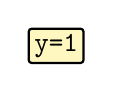
\begin{tikzpicture}[baseline=(ybox.base)]
				\node[
				draw=black,
				line width=0.8pt,
				fill=brightyellow,
				text=black,
				rectangle,
				rounded corners=1pt,
				inner sep=2pt
				] (ybox) {\texttt{y=1}};
			\end{tikzpicture}\\[-2.5pt]
			\begin{minipage}{0.8cm}
				\begin{lstlisting}[language=CustomPseudoCode,numbers=none,basicstyle=\tiny\ttfamily]
// end
				\end{lstlisting}
			\end{minipage}
		};
		
		%––– Response "1" –––
		\node[
		right=0.6cm of state2,
		draw=black,
		line width=0.8pt,
		fill=RedViolet!20,
		text=black,
		diamond,
		aspect=2,
		inner sep=2pt,
		scale=0.7,
		font=\Large
		] (resp1) {\texttt{1}};
		
		%––– Arrows –––
		\draw[->] (main) -- (state1);
		
		% Single transition label: X=0 -> X=1
		\draw[->] (state1) -- node[above] {%
			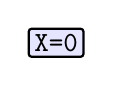
\begin{tikzpicture}[baseline=(a.base)]
				\node[draw=black,line width=0.8pt,fill=blue!10,rectangle,rounded corners=1pt,inner sep=2pt] (a) {\texttt{X=0}};
			\end{tikzpicture}
			$\to$
			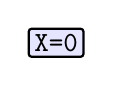
\begin{tikzpicture}[baseline=(b.base)]
				\node[draw=black,line width=0.8pt,fill=blue!10,rectangle,rounded corners=1pt,inner sep=2pt] (b) {\texttt{X=0}};
			\end{tikzpicture}
		} (state2);
		
		% To response "1"
		\draw[->] (state2) -- (resp1);
		
	\end{tikzpicture}
	
	\caption{Network System for interleaving executions of the program in Listing~\ref{lst:MotivatingExample1Ser}.}
\label{fig:code1ExampleNS}
\end{figure}



%\begin{figure}[!htbp]
%	\centering
%	\includegraphics[width=0.9\textwidth]{plots/code_1_NS.png}
%	\caption{Network System for interleaving executions of the program in Listing~\ref{lst:MotivatingExample1Ser}.}
%	\label{fig:code1ExampleNS}
%\end{figure}


%\begin{figure}[!htbp]
%	\centering
%	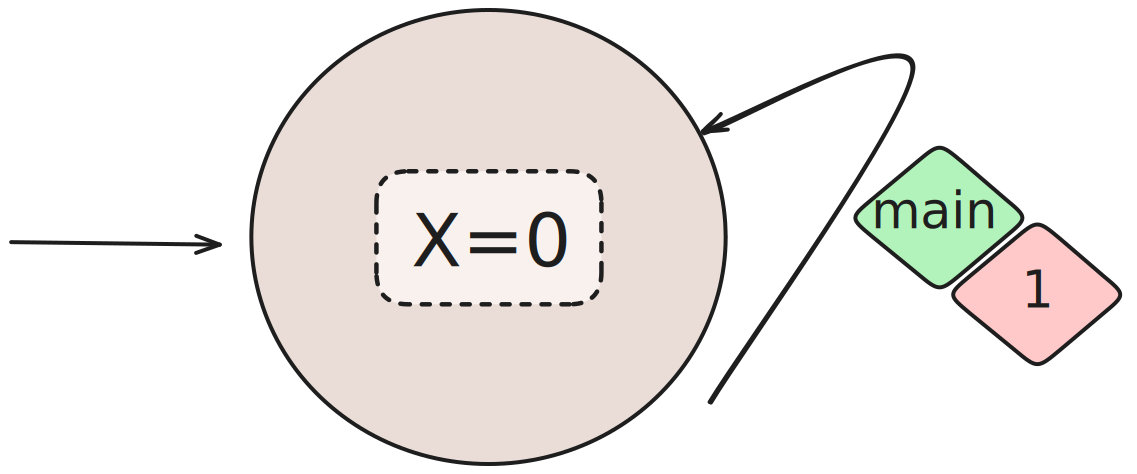
\includegraphics[width=0.35\textwidth]{plots/code_1_NFA.png}
%	\caption{NFA for serial executions of the program in Listing~\ref{lst:MotivatingExample1Ser}.}
%	\label{fig:code1ExampleNFA}
%\end{figure}


\begin{figure}  [!htbp]
	\centering
	% \includegraphics[width=0.48\textwidth,trim=0 0 0 0,clip]{plots/code_single_X0_NFA.pdf}
	
	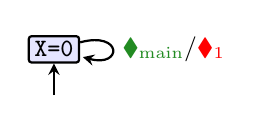
\begin{tikzpicture}[
		->,>=stealth,
		thick,
		node distance=2.5cm,
		state/.style={
			draw=black,
			line width=0.8pt,
			fill=blue!10,
			rectangle,
			rounded corners=1pt,
			inner sep=2pt,
			font=\small
		},
		every node/.style={font=\small}
		]
		% Single state
		\node[state] (X0) {\texttt{X=0}};
		
		% Initial state arrow
		\draw[->] ([yshift=-0.4cm]X0.south) -- (X0.south);
		
		% Self-loop with main/1 using the paper's colored lozenge notation
		\draw[->] (X0) edge[loop right]
		node[right] {${\color{ForestGreen}\blacklozenge_{\mathrm{main}}}/{\color{red}\blacklozenge_1}$} (X0);
	\end{tikzpicture}
	
	\caption{NFA for serial executions of the program in Listing~\ref{lst:MotivatingExample1Ser}.}
\label{fig:code1ExampleNFA}
\end{figure}




\begin{figure}[H]
	\centering
	\includegraphics[width=0.6\textwidth]{plots/code_1_PN_with_annotation.png}
	\caption{Petri net for interleaving executions of the program in Listing~\ref{lst:MotivatingExample1Ser}.}
	\label{fig:code1ExamplePN}
\end{figure}


%

\subsection{Translation Example: Listing~\ref{lst:MotivatingExample2NonSer}}
\label{appendix:subsec::Ex1B:NS}

The Network System, Serializability NFA, and Pet net of Listing~\ref{lst:MotivatingExample2NonSer} are depicted in the main text (see subsec.~\ref{subsec:SerToNsTranslation}).
%
We present in Fig.~\ref{fig:code2ExampleNSSecondPart} the mappings \(\delta\), $req$, and $resp$.

\begin{figure}[!htbp]
	\centering
	%–––– Network system diagram ––––
	% \includegraphics[width=\textwidth]{plots/code_2_NS.png}\\[1ex]
	
	%–––– req, resp, and δ definitions ––––
	\[
	\begin{array}{@{}r@{\;}l}
		req \coloneq & 
		\big\{
		\big[
		\begin{array}{c c c}
			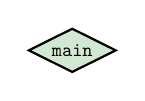
\begin{tikzpicture}[baseline=(textnode.base)]
				\node[
				draw=black,
				line width=0.8pt,
				fill=ForestGreen!20,
				text=black,
				diamond,
				aspect=2,
				inner sep=2pt,
				scale=0.7
				] (textnode) {\texttt{main}};
			\end{tikzpicture}
			&\!\!\rightarrow\!\!&
			\begin{array}{c}
				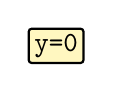
\begin{tikzpicture}[baseline=(ybox.base)]
					\node[
					draw=black,
					line width=0.8pt,
					fill=brightyellow,
					text=black,
					rectangle,
					rounded corners=1pt,
					inner sep=2pt
					] (ybox) {\texttt{y=0}};
				\end{tikzpicture}\vspace{-2pt}
				\\
				\begin{minipage}{0.20\linewidth}
					\begin{lstlisting}[language=CustomPseudoCode,numbers=none,basicstyle=\tiny\ttfamily]
X := 1 
yield 
y := X
X := 0
return y
					\end{lstlisting}
				\end{minipage}
			\end{array}
		\end{array}
		\big]
		\big\}
		\\[2em]
		resp \coloneq &
		\big\{
		\big[
		\begin{array}{c c c}
			\begin{array}{c}
				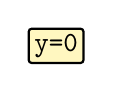
\begin{tikzpicture}[baseline=(ybox.base)]
					\node[
					draw=black,
					line width=0.8pt,
					fill=brightyellow,
					text=black,
					rectangle,
					rounded corners=1pt,
					inner sep=2pt
					] (ybox) {\texttt{y=0}};
				\end{tikzpicture}\vspace{-2pt}
				\\
				\begin{minipage}{0.11\linewidth}
					\begin{lstlisting}[language=CustomPseudoCode,numbers=none,basicstyle=\tiny\ttfamily]
// end
					\end{lstlisting}
				\end{minipage}
			\end{array}
			&\!\!\rightarrow\!\!&
			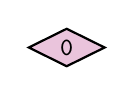
\begin{tikzpicture}[baseline=(textnode.base),scale=0.7]
				\node[
				draw=black,
				line width=0.8pt,
				fill=RedViolet!20,
				text=black,
				diamond,
				aspect=2,
				inner sep=2pt,
				font=\small
				] (textnode) {\texttt{0}};
			\end{tikzpicture}
		\end{array}
		\big]\,{},
		\big[
		\begin{array}{c c c}
			\begin{array}{c}
				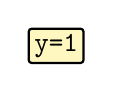
\begin{tikzpicture}[baseline=(ybox.base)]
					\node[
					draw=black,
					line width=0.8pt,
					fill=brightyellow,
					text=black,
					rectangle,
					rounded corners=1pt,
					inner sep=2pt
					] (ybox) {\texttt{y=1}};
				\end{tikzpicture}\vspace{-2pt}
				\\
				\begin{minipage}{0.11\linewidth}
					\begin{lstlisting}[language=CustomPseudoCode,numbers=none,basicstyle=\tiny\ttfamily]
// end
					\end{lstlisting}
				\end{minipage}
			\end{array}
			&\!\!\rightarrow\!\!&
			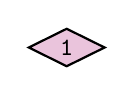
\begin{tikzpicture}[baseline=(textnode.base),scale=0.7]
				\node[
				draw=black,
				line width=0.8pt,
				fill=RedViolet!20,
				text=black,
				diamond,
				aspect=2,
				inner sep=2pt,
				font=\small
				] (textnode) {\texttt{1}};
			\end{tikzpicture}
		\end{array}
		\big]
		\big\}
		\\[2em]
		\delta \coloneq & 
		\big\{\big[(
		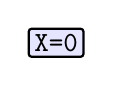
\begin{tikzpicture}[baseline=(ybox.base)]
			\node[
			draw=black,
			line width=0.8pt,
			fill=blue!10,
			text=black,
			rectangle,
			rounded corners=1pt,
			inner sep=2pt
			] (ybox) {\texttt{X=0}};
		\end{tikzpicture}\,{},
		\begin{array}{c}
			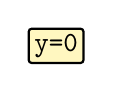
\begin{tikzpicture}[baseline=(ybox.base)]
				\node[
				draw=black,
				line width=0.8pt,
				fill=brightyellow,
				text=black,
				rectangle,
				rounded corners=1pt,
				inner sep=2pt
				] (ybox) {\texttt{y=0}};
			\end{tikzpicture}\vspace{-2pt}
			\\
			\begin{minipage}{0.14\linewidth}
				\begin{lstlisting}[language=CustomPseudoCode,numbers=none,basicstyle=\tiny\ttfamily]
X := 1
yield
y := X
X := 0
return y
				\end{lstlisting}
			\end{minipage}
		\end{array}
		)
		\;\rightarrow\;
		(
		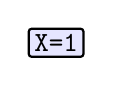
\begin{tikzpicture}[baseline=(ybox.base)]
			\node[
			draw=black,
			line width=0.8pt,
			fill=blue!10,
			text=black,
			rectangle,
			rounded corners=1pt,
			inner sep=2pt
			] (ybox) {\texttt{X=1}};
		\end{tikzpicture}\,{},
		\begin{array}{c}
			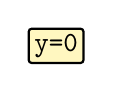
\begin{tikzpicture}[baseline=(ybox.base)]
				\node[
				draw=black,
				line width=0.8pt,
				fill=brightyellow,
				text=black,
				rectangle,
				rounded corners=1pt,
				inner sep=2pt
				] (ybox) {\texttt{y=0}};
			\end{tikzpicture}\vspace{-2pt}
			\\
			\begin{minipage}{0.14\linewidth}
				\begin{lstlisting}[language=CustomPseudoCode,numbers=none,basicstyle=\tiny\ttfamily]
y := X
X := 0
return y
				\end{lstlisting}
			\end{minipage}
		\end{array}
		)
		\big],
		\\[0.5em]
		& \phantom{\big\{}
		\big[(
		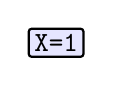
\begin{tikzpicture}[baseline=(ybox.base)]
			\node[
			draw=black,
			line width=0.8pt,
			fill=blue!10,
			text=black,
			rectangle,
			rounded corners=1pt,
			inner sep=2pt
			] (ybox) {\texttt{X=1}};
		\end{tikzpicture}\,{},
		\begin{array}{c}
			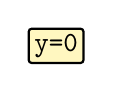
\begin{tikzpicture}[baseline=(ybox.base)]
				\node[
				draw=black,
				line width=0.8pt,
				fill=brightyellow,
				text=black,
				rectangle,
				rounded corners=1pt,
				inner sep=2pt
				] (ybox) {\texttt{y=0}};
			\end{tikzpicture}\vspace{-2pt}
			\\
			\begin{minipage}{0.14\linewidth}
				\begin{lstlisting}[language=CustomPseudoCode,numbers=none,basicstyle=\tiny\ttfamily]
y := X
X := 0
return y
				\end{lstlisting}
			\end{minipage}
		\end{array}
		)
		\;\rightarrow\;
		(
		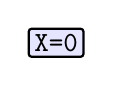
\begin{tikzpicture}[baseline=(ybox.base)]
			\node[
			draw=black,
			line width=0.8pt,
			fill=blue!10,
			text=black,
			rectangle,
			rounded corners=1pt,
			inner sep=2pt
			] (ybox) {\texttt{X=0}};
		\end{tikzpicture}\,{},
		\begin{array}{c}
			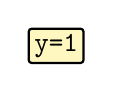
\begin{tikzpicture}[baseline=(ybox.base)]
				\node[
				draw=black,
				line width=0.8pt,
				fill=brightyellow,
				text=black,
				rectangle,
				rounded corners=1pt,
				inner sep=2pt
				] (ybox) {\texttt{y=1}};
			\end{tikzpicture}
			\vspace{-2pt}
			\\
			\begin{minipage}{0.11\linewidth}
				\begin{lstlisting}[language=CustomPseudoCode,numbers=none,basicstyle=\tiny\ttfamily]
// end
				\end{lstlisting}
			\end{minipage}
		\end{array}
		)
		\big],
		\ldots
		\big\}
	\end{array}
	\]
	\caption{The \(\delta\) transition function, and the \(req\) and \(resp\) mappings for the program in Listing~\ref{lst:MotivatingExample2NonSer}.}
	\label{fig:code2ExampleNSSecondPart}
\end{figure}



\subsection{Translation Example: Listing~\ref{lst:MotivatingExample3Ser}}
\label{appendix:subsec:Ex1C:NS}


For our third motivating example, presented in Listing~\ref{lst:MotivatingExample3Ser}, we denote the Network System in Fig.~\ref{fig:code3ExampleNS}, the Serializability NFA in Fig.~\ref{fig:code3ExampleNFA}, and the Interleaving Petri net in Fig.~\ref{fig:code3ExamplePN}.

%\begin{minipage}[t]{0.3\textwidth}
%	\begin{lstlisting}[caption={With yield and lock (serializable)}]
%		request foo: 
%			// lock
%			while (L == 1): 
%				yield
%			L := 1 
%		
%			X := 1
%			yield
%			y := X 
%			X := 0
%		
%			// unlock    
%			L := 0
%			return y 
%	\end{lstlisting}
%\end{minipage}
%
%This program corresponds to the following Network System (NS):

%\begin{figure}[!htbp]
%	\centering
%	\includegraphics[width=1.1\textwidth]{plots/code_3_NS.png}
%	\caption{Network System for interleaving executions of the program in Listing~\ref{lst:MotivatingExample3Ser}.}
%	\label{fig:code3ExampleNS}
%\end{figure}


\begin{figure}[!htbp]
	\centering
	% \includegraphics[width=\textwidth]{plots/code_locking_NS.png}\\[1ex]
	
	\begin{tikzpicture}[
		node distance=1.5cm and 2.5cm,
		>=stealth,
		thick,
		every node/.style={font=\small}
		]
		%–––– Request (green diamond) ––––
		\node[
		draw=black,
		line width=0.8pt,
		fill=ForestGreen!20,
		text=black,
		diamond,
		aspect=2,
		inner sep=2pt,
		scale=0.7
		] (main) {\texttt{main}};
		
		%–––– State 1: y=0 + locked program ––––
		\node[right=0.7cm of main, align=center] (state1) {
			\begin{tikzpicture}[baseline=(ybox.base)]
				\node[
				draw=black,
				line width=0.8pt,
				fill=brightyellow,
				text=black,
				rectangle,
				rounded corners=1pt,
				inner sep=2pt
				] (ybox) {\texttt{y=0}};
			\end{tikzpicture}\\[-2.5pt]
			\begin{minipage}{2.6cm}
				\begin{lstlisting}[language=CustomPseudoCode,numbers=none,basicstyle=\tiny\ttfamily]
while (L == 1):
	yield
L := 1

X := 1
yield
y := X
X := 0

// unlock
L := 0
return y
				\end{lstlisting}
			\end{minipage}
		};
		
		%–––– State 2: y=0 + tail program ––––
		\node[right=of state1, xshift=12mm, align=center] (state2) {
			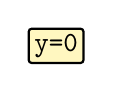
\begin{tikzpicture}[baseline=(ybox.base)]
				\node[
				draw=black,
				line width=0.8pt,
				fill=brightyellow,
				text=black,
				rectangle,
				rounded corners=1pt,
				inner sep=2pt
				] (ybox) {\texttt{y=0}};
			\end{tikzpicture}\\[-2.5pt]
			\begin{minipage}{2.0cm}
				\begin{lstlisting}[language=CustomPseudoCode,numbers=none,basicstyle=\tiny\ttfamily]
y := X
X := 0

// unlock
L := 0
return y
				\end{lstlisting}
			\end{minipage}
		};
		
		%–––– State 3 (top-right): //end, y=0 ––––
		\node[above right=-0.5cm and 2.2cm of state2, align=center] (state3) {
			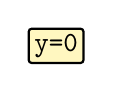
\begin{tikzpicture}[baseline=(ybox.base)]
				\node[
				draw=black,
				line width=0.8pt,
				fill=brightyellow,
				text=black,
				rectangle,
				rounded corners=1pt,
				inner sep=2pt
				] (ybox) {\texttt{y=0}};
			\end{tikzpicture}\\[-2.5pt]
			\begin{minipage}{0.9cm}
				\begin{lstlisting}[language=CustomPseudoCode,numbers=none,basicstyle=\tiny\ttfamily]
// end
				\end{lstlisting}
			\end{minipage}
		};
		
		%–––– State 4 (bottom-right): //end, y=1 ––––
		\node[below right=-0.2cm and 2.2cm of state2, align=center] (state4) {
			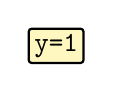
\begin{tikzpicture}[baseline=(ybox.base)]
				\node[
				draw=black,
				line width=0.8pt,
				fill=brightyellow,
				text=black,
				rectangle,
				rounded corners=1pt,
				inner sep=2pt
				] (ybox) {\texttt{y=1}};
			\end{tikzpicture}\\[-2.5pt]
			\begin{minipage}{0.9cm}
				\begin{lstlisting}[language=CustomPseudoCode,numbers=none,basicstyle=\tiny\ttfamily]
// end
				\end{lstlisting}
			\end{minipage}
		};
		
		%–––– Responses ––––
		\node[
		right=0.6cm of state3,
		draw=black,
		line width=0.8pt,
		fill=RedViolet!20,
		text=black,
		diamond,
		aspect=2,
		inner sep=2pt,
		scale=0.7,
		font=\Large
		] (resp0) {\texttt{0}};
		
		\node[
		right=0.6cm of state4,
		draw=black,
		line width=0.8pt,
		fill=RedViolet!20,
		text=black,
		diamond,
		aspect=2,
		inner sep=2pt,
		scale=0.7,
		font=\Large
		] (resp1) {\texttt{1}};
		
		%–––– Arrows ––––
		\draw[->] (main) -- (state1);
		
		% Self-loop on state1: (X=1,L=1) -> (X=1,L=1)
		\draw[->] (state1) edge[loop above]
		node[above] {%
			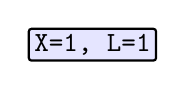
\begin{tikzpicture}[baseline=(a.base)]
				\node[draw=black,line width=0.8pt,fill=blue!10,rectangle,rounded corners=1pt,inner sep=2pt] (a) {\texttt{X=1, L=1}};
			\end{tikzpicture}
			$\to$
			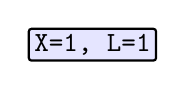
\begin{tikzpicture}[baseline=(b.base)]
				\node[draw=black,line width=0.8pt,fill=blue!10,rectangle,rounded corners=1pt,inner sep=2pt] (b) {\texttt{X=1, L=1}};
			\end{tikzpicture}
		} (state1);
		
		% Transition state1 -> state2: (X=0,L=0) -> (X=1,L=1)
		\draw[->] (state1) -- node[above] {%
			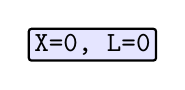
\begin{tikzpicture}[baseline=(a.base)]
				\node[draw=black,line width=0.8pt,fill=blue!10,rectangle,rounded corners=1pt,inner sep=2pt] (a) {\texttt{X=0, L=0}};
			\end{tikzpicture}
			$\to$
			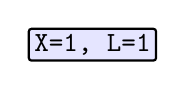
\begin{tikzpicture}[baseline=(b.base)]
				\node[draw=black,line width=0.8pt,fill=blue!10,rectangle,rounded corners=1pt,inner sep=2pt] (b) {\texttt{X=1, L=1}};
			\end{tikzpicture}
		} (state2);
		
		% Transition state2 -> state3: (X=0,L=0) -> (X=0,L=0)
		\draw[->] ([yshift=4pt]state2.east) to[out=50,in=180]
		node[above,sloped] {%
			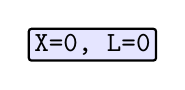
\begin{tikzpicture}[baseline=(a.base)]
				\node[draw=black,line width=0.8pt,fill=blue!10,rectangle,rounded corners=1pt,inner sep=2pt] (a) {\texttt{X=0, L=0}};
			\end{tikzpicture}
			$\to$
			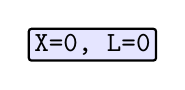
\begin{tikzpicture}[baseline=(b.base)]
				\node[draw=black,line width=0.8pt,fill=blue!10,rectangle,rounded corners=1pt,inner sep=2pt] (b) {\texttt{X=0, L=0}};
			\end{tikzpicture}
		} (state3.west);
		
		% Transition state2 -> state4: (X=1,L=1) -> (X=0,L=0)
		\draw[->] ([yshift=-16pt]state2.east) to[out=-50,in=180]
		node[below,sloped] {%
			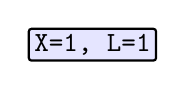
\begin{tikzpicture}[baseline=(a.base)]
				\node[draw=black,line width=0.8pt,fill=blue!10,rectangle,rounded corners=1pt,inner sep=2pt] (a) {\texttt{X=1, L=1}};
			\end{tikzpicture}
			$\to$
			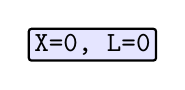
\begin{tikzpicture}[baseline=(b.base)]
				\node[draw=black,line width=0.8pt,fill=blue!10,rectangle,rounded corners=1pt,inner sep=2pt] (b) {\texttt{X=0, L=0}};
			\end{tikzpicture}
		} (state4.west);
		
		% To responses
		\draw[->] (state3) -- (resp0);
		\draw[->] (state4) -- (resp1);
		
	\end{tikzpicture}
	
	\caption{Network System for interleaving executions of the program in Listing~\ref{lst:MotivatingExample3Ser}.}
\label{fig:code3ExampleNS}
\end{figure}



%\begin{figure}[!htbp]
%	\centering
%	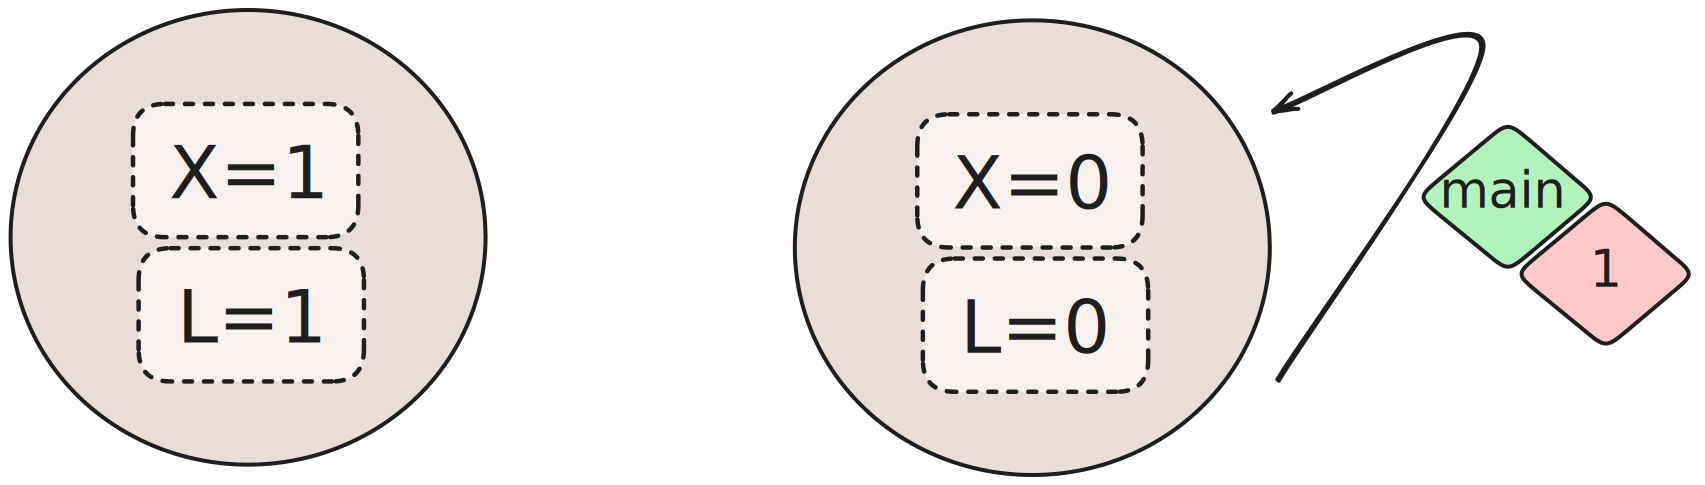
\includegraphics[width=0.4\textwidth]{plots/code_3_NFA.png}
%	\caption{NFA for serial executions of the program in Listing~\ref{lst:MotivatingExample3Ser}.}
%	\label{fig:code3ExampleNFA}
%\end{figure}


\begin{figure}  [!htbp]
	\centering
	% \includegraphics[width=0.48\textwidth,trim=0 0 0 0,clip]{plots/code_two_states_XL_NFA.pdf}
	
	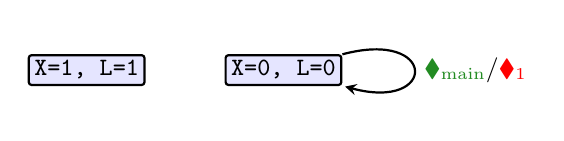
\begin{tikzpicture}[
		->,>=stealth,
		thick,
		node distance=2.5cm,
		state/.style={
			draw=black,
			line width=0.8pt,
			fill=blue!10,
			rectangle,
			rounded corners=1pt,
			inner sep=2pt,
			font=\small
		},
		every node/.style={font=\small}
		]
		% States
		\node[state] (X1L1) {\texttt{X=1, L=1}};
		\node[state, right of=X1L1] (X0L0) {\texttt{X=0, L=0}};
		
		% No edges to or from X=1, L=1 (isolated)
		
		% Self-loop on X=0, L=0 with main/1 (colored lozenge notation)
		\draw[->] (X0L0) edge[loop right]
		node[right] {${\color{ForestGreen}\blacklozenge_{\mathrm{main}}}/{\color{red}\blacklozenge_1}$} (X0L0);
	\end{tikzpicture}
	
	\caption{NFA for serial executions of the program in Listing~\ref{lst:MotivatingExample3Ser}.}
\label{fig:code3ExampleNFA}
\end{figure}




\begin{figure}[!htbp]
	\centering
	\includegraphics[width=0.8\textwidth]{plots/code_3_PN_with_annotation.png}
	\caption{Petri net for interleaving executions of the program in Listing~\ref{lst:MotivatingExample3Ser}.}
	\label{fig:code3ExamplePN}
\end{figure}

%\newpage
\clearpage

\section{Translating Network Systems to Petri Nets}
\label{appendix:NS-to-PN-formulation}


We denote with \(\mathbf0\) a zero vector of dimension \(|P|\), and with \(\mathbf1_{p}\) a \(|P|\)-sized indicator vector that has 0 in every coordinate except the one corresponding to place \(p \in P\), which has 1. 
% 
The flow functions $\mathsf{pre},\mathsf{post}:T\to\{0,1\}^{|P|}$ assign to each transition $t$ a binary vector over $P$ whose $1$-entries mark the places from which tokens are consumed (for $\mathsf{pre}(t)$) and to which tokens are produced (for $\mathsf{post}(t)$) when $t$ fires.
A transition $t$ is enabled at $M$ iff $\mathsf{pre}(t)\le M$ (component-wise); firing yields
\(
M\xrightarrow{t}M' \quad\text{where}\quad M' = M-\mathsf{pre}(t)+\mathsf{post}(t)
\).	

\medskip
\textit{Construction.}
We generate the Petri net:
\[
N_{\mathrm{int}}(\mathcal S)
= (P,\,T,\,\mathsf{pre},\,\mathsf{post},\,M_0),
\]
where
\[
P
=
P_G \;\cup\; P_{REQ,L} \;\cup\; P_{REQ,RESP}
\]

for 
\[
\begin{aligned}
	P_G
	&= \{\,p_g \mid g\in G\},\quad
	P_{REQ,L}
	= \bigl\{\,p_{({\color{ForestGreen}\blacklozenge_{\mathit{req}}},\ell)}
	\mid {\color{ForestGreen}\blacklozenge_{\mathit{req}}}\in\mathit{REQ},\,\ell\in  L\bigr\},\\[1ex]
	P_{REQ,RESP}
	&= \bigl\{\,p_{({\color{ForestGreen}\blacklozenge_{\mathit{req}}}/{\color{red}\blacklozenge_{\mathit{resp}}})}
	\mid {\color{ForestGreen}\blacklozenge_{\mathit{req}}}\in\mathit{REQ},\,
	{\color{red}\blacklozenge_{\mathit{resp}}}\in\mathit{RESP}\bigr\}.
\end{aligned}
\]


%	\[
%	\begin{aligned}
	%		P_G &= \{\,p_g \mid g\in G\},\;\,
	%		P_{REQ,L} = \{\,p_{{\color{ForestGreen}\blacklozenge_{\mathit{req}}}/\ell}
	%		\mid {\color{ForestGreen}\blacklozenge_{\mathit{req}}}\in\mathit{REQ},\,\ell\in L\},\\
	%		P_{REQ,RESP} &= \{\,p_{{\color{ForestGreen}\blacklozenge_{\mathit{req}}}/{\color{red}\blacklozenge_{\mathit{resp}}}}
	%		\mid {\color{ForestGreen}\blacklozenge_{\mathit{req}}}\in\mathit{REQ},\,
	%		{\color{red}\blacklozenge_{\mathit{resp}}}\in\mathit{RESP}\}.
	%	\end{aligned}
%	\]

%	\[
%	P_G 
%	= \{\,p_g \mid g\in G\}
%	\quad 
%%	P_L 
%%	= \{\,p_\ell \mid \ell\in L\}
%%	\quad
%	P_{REQ,L} =
%	\{\,p_{{\color{ForestGreen}\blacklozenge_{\mathit{req}}}/\ell} \mid
%	{\color{ForestGreen}\blacklozenge_{\mathit{req}}}\in \mathit{REQ}, \ell\in L\},%\\
%	\quad
%	P_{REQ,RESP}=
%	\{\,p_{{\color{ForestGreen}\blacklozenge_{\mathit{req}}}/{\color{red}\blacklozenge_{\mathit{resp}}}} \mid
%	{\color{ForestGreen}\blacklozenge_{\mathit{req}}}\in \mathit{REQ}, {\color{red}\blacklozenge_{\mathit{resp}}}\in \mathit{RESP}\},
%	\]
%	\{\,p_{{\color{ForestGreen}\blacklozenge_{\mathit{req}}}/{\color{red}\blacklozenge_{\mathit{resp}}}} \mid
%	{\color{ForestGreen}\blacklozenge_{\mathit{req}}}\in \mathit{REQ}, {\color{red}\blacklozenge_{\mathit{resp}}}\in \mathit{RESP}\},
%	\]

%	\[
%	P_{REQ,RESP}=
%	\{\,p_{{\color{ForestGreen}\blacklozenge_{\mathit{req}}}/{\color{red}\blacklozenge_{\mathit{resp}}}} \mid
%	{\color{ForestGreen}\blacklozenge_{\mathit{req}}}\in \mathit{REQ}, {\color{red}\blacklozenge_{\mathit{resp}}}\in \mathit{RESP}\},
%	\]

with \(G\) being the set of global states, \(L\) being the set of local states (in the case of a \toolname-derived NS, this is the coupling of the local variable assignments of an in-flight request and its remaining \toolname{} program to execute), \(\mathit{REQ}\) denotes the request labels; and \(\mathit{RESP}\) denotes the response labels.

\medskip
Transitions are partitioned as:
\[
T = T_{\mathit{req}} \;\cup\; T_{\delta}\;\cup\;T_{\mathit{resp}}
\]
where

%	\[
%	T_{\mathit{req}} = \{\,t_{({\color{ForestGreen}\blacklozenge_{\mathit{req}}},\ell)} \mid {(\color{ForestGreen}\blacklozenge_{\mathit{req}}},\ell)\in\mathit{req}\},\quad
%	T_{\delta} = \{\,t_{(\ell,g)\to(\ell',g')} \mid (\ell,g)\xrightarrow{}(\ell',g')\in\delta\},\quad
%	T_{\mathit{resp}} = \{\,t_{(\ell,{\color{red}\blacklozenge_{\mathit{resp}}})} \mid (\ell,{\color{red}\blacklozenge_{\mathit{resp}}})\in\mathit{resp}\}.
%	\]

\begin{align*}
	T_{\mathit{req}}
	&= \{\,t_{({\color{ForestGreen}\blacklozenge_{\mathit{req}}},\ell)} \mid {(\color{ForestGreen}\blacklozenge_{\mathit{req}}},\ell)\in\mathit{req}\},\\[1ex]
	T_{\delta}
	&= \bigl\{\,t_{((\ell,g),(\ell',g'))} 
	\mid ((\ell,g),(\ell',g'))\in\delta\bigr\},\quad
	T_{\mathit{resp}}
	= \{\,t_{(\ell,{\color{red}\blacklozenge_{\mathit{resp}}})} \mid (\ell,{\color{red}\blacklozenge_{\mathit{resp}}})\in\mathit{resp}\}.
\end{align*}



%\smallskip
%Given a local state \(\ell\) which resulted from a request \({\color{ForestGreen}\blacklozenge_{\mathit{req}}}\) (either directly or downstream due to program execution) --- the transitions are:
Their \(\mathsf{pre}\) and \(\mathsf{post}\) flow functions are:
\[
\begin{alignedat}{3}
	\mathsf{pre}\bigl(t_{({\color{ForestGreen}\blacklozenge_{\mathit{req}}},\ell)}\bigr)
	&= \mathbf0, &
	\mathsf{post}\bigl(t_{({\color{ForestGreen}\blacklozenge_{\mathit{req}}},\ell)}\bigr)
	&= \mathbf1_{p_{({\color{ForestGreen}\blacklozenge_{\mathit{req}}},\ell)}}, 
	&&\text{for }({\color{ForestGreen}\blacklozenge_{\mathit{req}}},\ell)\in\mathit{req},\\
	\mathsf{pre}\bigl(t_{((\ell,g),(\ell',g'))}\bigr)
	&= \mathbf1_{p_{({\color{ForestGreen}\blacklozenge_{\mathit{req}}},\ell)}} + \mathbf1_{p_g}, &
	\mathsf{post}\bigl(t_{((\ell,g),(\ell',g'))}\bigr)
	&= \mathbf1_{p_{({\color{ForestGreen}\blacklozenge_{\mathit{req}}},\ell')}} + \mathbf1_{p_{g'}}, 
	&&\text{for }{{\color{ForestGreen}\blacklozenge_{\mathit{req}}}\in\mathit{REQ}}, ((\ell,g),(\ell',g'))\in\delta,\\
	\mathsf{pre}\bigl(t_{(\ell,{\color{red}\blacklozenge_{\mathit{resp}}})}\bigr)
	&= \mathbf1_{p_{({\color{ForestGreen}\blacklozenge_{\mathit{req}}},\ell)}}, &
	\mathsf{post}\bigl(t_{(\ell,{\color{red}\blacklozenge_{\mathit{resp}}})}\bigr)
	&= \mathbf1_{p_{({\color{ForestGreen}\blacklozenge_{\mathit{req}}}/{\color{red}\blacklozenge_{\mathit{resp}}})}}, 
	&&\text{for }{{\color{ForestGreen}\blacklozenge_{\mathit{req}}}\in\mathit{REQ},(\ell,\color{red}\blacklozenge_{\mathit{resp}}})\in\mathit{resp}
	%\ %(\ell\text{ the matching local state).
		%		}
\end{alignedat}
\]

Where for the last two cases, \({\color{ForestGreen}\blacklozenge_{\mathit{req}}}\) concerns requests that eventually give rise to a local state \(\ell \in L\) that originated downstream (during execution).

\medskip
The initial marking is a single token on the single place representing the initial global state $g_0$ of the NS:
\[
M_0(p_{g_0}) = 1,
\quad
M_0(p) = 0 \text{ for all }p\neq p_{g_0},
\]
%	where \(g_0\) is the initial global state of the network system \(\mathcal S\).  



Define the projection \(\pi\) to solely include the markings of places representing completed request/response pairs.
% (with the exception of a single token on a state in \(P_G\)).
%\[
%\pi \;:\;\mathbb N^P \;\longrightarrow\;\mathbb N^{P_R}
%\quad\bigl(\pi(M)\bigr)(p_{({{\color{ForestGreen}\blacklozenge_{\mathit{req}}}/{\color{red}\blacklozenge_{\mathit{resp}}}})})\;=\;M(p_{({{\color{ForestGreen}\blacklozenge_{\mathit{req}}}/{\color{red}\blacklozenge_{\mathit{resp}}}})})\text{ for }p_{({{\color{ForestGreen}\blacklozenge_{\mathit{req}}}/{\color{red}\blacklozenge_{\mathit{resp}}}})}\in P_{REQ,RESP}.
%\]
Then, the multiset of all  (${{\color{ForestGreen}\blacklozenge_{\mathit{req}}}/{\color{red}\blacklozenge_{\mathit{resp}}}}$) pairs of the NS, obtained by \textit{any} interleaving, is:
\[
\mathsf{Int}(\mathcal S)
\;=\;
\bigl\{\;\pi(M)\;\bigm|\;M_0 \xrightarrow{}^{*} M\text{ in }N_{\mathrm{int}}(\mathcal S)\bigr\}.
\]

\section{Example: Serializable Program}
\label{appendix:ns-serializable}


Now, we observe again the adjusted program with a spin-lock (as previously described in Listing~\ref{lst:MotivatingExample3Ser}), of which we depicted figures of the corresponding Network System (Fig.~\ref{fig:code3ExampleNS}), Serializability NFA (Fig.~\ref{fig:code3ExampleNFA}), and the interleaving Petri net (Fig.~\ref{fig:code3ExamplePN}) in Appendix~\ref{appendix:MoreNsExamples}.
%
In this case, serializability corresponds to the Petri net being unable to reach a marking satisfying the same semilinear formula \(\mathcal {F}\) as in the non-serializable case described in the main text (subsec.~\ref{subsec:SerToNsTranslation}):

\[
\mathcal {F}:
\quad
P_1 = 0 \wedge 
\textcolor{blue}{P_2} \ge 0 \wedge \textcolor{blue}{P_3} \ge 0  \wedge P_4 = 0
\wedge P_5 = 0 \wedge P_6 = 0 \wedge \textcolor{red}{P_7} \ge 0 \wedge \textcolor{red}{P_8} \ge 1.
\]

% (note however, that this is not always the case). 
%(but this time each place $P_i$ corresponds to the new PN). 
%following formula:
%
%\[
%\textcolor{blue}
%P_1 = 0 \wedge 
%{P_2} \ge 0 \wedge \textcolor{blue}{P_3} \ge 0  \wedge P_4 = 0
%\wedge P_5 = 0 \wedge P_6 = 0 \wedge \textcolor{red}{P_7} = 0 \wedge \textcolor{red}{P_8} \ge 1.
%\]


In addition, although the target set is the same as in the previous example, the Petri net places $(P_1,\ldots,P_8)$ encode different states that correspond to the updated network system. For instance, now each place in the PN that encodes a global state accounts for two global variables, \texttt{X} and \texttt{L}, and the initial global state corresponds to the place encoding the initial assignment \textcolor{blue}{[X=0, L=0]}, etc.
%
Furthermore, unlike the case in Listing~\ref{lst:MotivatingExample2NonSer} (covered in subsec.~\ref{subsec:SerToNsTranslation}), this target set of markings (encoding request/response pairs of non-serial executions) is \textit{unreachable}, as witnessed by the inductive invariant:


\[
\begin{aligned}
	&(P_{1},\textcolor{blue}{P_{2}},\textcolor{blue}{P_{3}},P_{4},P_{5},P_{6},\textcolor{red}{P_{7}},\textcolor{red}{P_{8}})
	\;\mapsto\;\\
	&\quad
	\exists\,e_{0},\dots,e_{5}\ge0.\;
	\Bigl(
	e_{2}-e_{1}+\textcolor{blue}{P_{3}}-1=0\;\land\;
	e_{2}+P_{1}-e_{5}=0\;\land\;
	P_{5}-e_{1}+e_{4}=0\;\land\\
	&\qquad\quad
	-\,e_{4}+\textcolor{red}{P_{7}}=0\;\land\;
	P_{6}+e_{3}-e_{0}=0\;\land\;
	\textcolor{red}{P_{8}}-e_{3}=0\;\land\\
	&\qquad\quad
	-\,e_{2}+e_{1}+e_{0}+P_{4}=0\;\land\;
	-\,e_{2}+e_{1}+\textcolor{blue}{P_{2}}=0
	\Bigr)
	\;\land\;
	\bigl(P_{4}-1\ge0\;\lor\;\textcolor{blue}{P_{3}}-1\ge0\bigr).
\end{aligned}
\]


We then revert and project it on the request/response pairs of the network system.
%
We get the following inductive invariants for each of the two (reachable) global states:

\begin{proof}
	
	\medskip\noindent
	For global state \textcolor{blue}{[L=0,X=0]} the projected invariant is:
	\[
	\bigl(\,\text{\color{ForestGreen}$\blacklozenge_{\text{main}}$}/\text{\color{red}$\blacklozenge_{0}$},\;
	\text{\color{ForestGreen}$\blacklozenge_{\text{main}}$}/\text{\color{red}$\blacklozenge_{1}$}\bigr)
	\;\mapsto\;
	\exists\,e_{0},\dots,e_{5}\ge0.\;
	\begin{aligned}[t]
		& e_{2}-e_{1}=0,\quad
		e_{2}-e_{5}=0,\quad
		-e_{1}+e_{4}=0,\\
		& -e_{4}+\bigl(\text{\color{ForestGreen}$\blacklozenge_{\text{main}}$}/\text{\color{red}$\blacklozenge_{1}$}\bigr)=0,\quad
		-e_{0}+e_{3}=0,\\
		& -e_{3}+\bigl(\text{\color{ForestGreen}$\blacklozenge_{\text{main}}$}/\text{\color{red}$\blacklozenge_{0}$}\bigr)=0,\quad
		-e_{2}+e_{1}+e_{0}=0,\\
		& -e_{2}+e_{1}=0.
	\end{aligned}
	\]
	\noindent From 
	\[e_{1}=e_{2}=e_{4}=e_{5}=(\;
	\text{\color{ForestGreen}$\blacklozenge_{\text{main}}$}/\text{\color{red}$\blacklozenge_{1}$}),\;
	e_{0}=e_{3}=
	(\text{\color{ForestGreen}$\blacklozenge_{\text{main}}$}/\text{\color{red}$\blacklozenge_{0}$})
	\]
	
	it follows that \[-e_{2}+e_{1}+e_{0}=0\;\Longrightarrow\;e_{0}=0,\]
	
	thus: 
	\[
	(	\text{\color{ForestGreen}$\blacklozenge_{\text{main}}$}/\text{\color{red}$\blacklozenge_{0}$})
	=0 \quad \text{and} \quad (	\text{\color{ForestGreen}$\blacklozenge_{\text{main}}$}/\text{\color{red}$\blacklozenge_{1}$})
	=0
	\]
	
	indicating that  (\(\text{\color{ForestGreen}$\blacklozenge_{\text{main}}$}/\text{\color{red}$\blacklozenge_{0}$}\)) cannot be obtained from the global state
	\textcolor{blue}{[L=0,X=0]}.
	
	\medskip\noindent
	In the second case, for the global state \textcolor{blue}{[L=1, X=1]}
	the projected invariant is:
	
	
	\[
	\bigl(\,\text{\color{ForestGreen}$\blacklozenge_{\text{main}}$}/\text{\color{red}$\blacklozenge_{0}$},\;
	\text{\color{ForestGreen}$\blacklozenge_{\text{main}}$}/\text{\color{red}$\blacklozenge_{1}$}\bigr)
	\;\mapsto\;
	\exists\,e_{0},\dots,e_{5}.\;\bot,
	\]
	which is unsatisfiable. Hence, no completed request/response pair, and in particular, no (\(\text{\color{ForestGreen}$\blacklozenge_{\text{main}}$}/\text{\color{red}$\blacklozenge_{0}$}\)) pair can be produced from this state via \textit{any} execution. Intuitively, this aligns with the fact that there cannot be any output generated via an interleaving, given that the spin-lock is acquired (\textcolor{blue}{[L=1]}).
	%	\guy{Mark/Jules is this part correct?}
	
	\medskip
	\noindent\textbf{Conclusion.}
	In every reachable state, no request/response pair of the form
	($	\text{\color{ForestGreen}$\blacklozenge_{\text{main}}$}/\text{\color{red}$\blacklozenge_{0}$})
	$
	can occur. Consequently, the only possible pairs are
	($	\text{\color{ForestGreen}$\blacklozenge_{\text{main}}$}/\text{\color{red}$\blacklozenge_{1}$})
	$,
	all of which lie within the NFA’s language for serial executions (Fig.~\ref{fig:code3ExampleNFA}).
	Hence, the program is serializable. Moreover, as proven in subsection~\ref{appendix:subsec:InductiveInvariantExample},
	these invariants are inductive: they hold in the initial state and are preserved under every transition.
\end{proof}

%	\medskip\noindent
%	\textbf{Conclusion.}
%	In all reachable states
%	it holds that there cannot be any request/response pair of type
%	(	$	\text{\color{ForestGreen}$\blacklozenge_{\text{main}}$}/\text{\color{red}$\blacklozenge_{0}$}
%	$).
%	%
%	Furthermore, this indicates that the only attainable request/response pairs are of the form 	($	\text{\color{ForestGreen}$\blacklozenge_{\text{main}}$}/\text{\color{red}$\blacklozenge_{1}$})
%	$, which are included in the language of of NFA for serial executions. Thus, this program is serializable.
%	%
%	We further show (in Appendix~\ref{appendix:InductiveInvariantExample}) that these invariants are \textit{inductive}: they encompass the system’s initial state and, once satisfied, remain true for all subsequent executions.




%\newpage


%\subsection{Time/Space Complexity}
%
%\guy{Should we add something about time/space complexity?}

%\newpage

\subsection{Proof of Inductive Invariant}
\label{appendix:subsec:InductiveInvariantExample}


\begin{proof}
	
	Define the predicate
	\[
	\begin{aligned}
		I(P_{1},\dots,\textcolor{red}{P_{8}})
		:={}&
		(P_{1},\textcolor{blue}{P_{2}},\textcolor{blue}{P_{3}},P_{4},P_{5},P_{6},\textcolor{red}{P_{7}},\textcolor{red}{P_{8}})
		\;\mapsto\;\\
		&\quad
		\exists\,e_{0},\dots,e_{5}\ge0.\;
		\Bigl(
		e_{2}-e_{1}+\textcolor{blue}{P_{3}}-1=0\;\land\;
		e_{2}+P_{1}-e_{5}=0\;\land\;
		P_{5}-e_{1}+e_{4}=0\;\land\\
		&\qquad\quad
		-\,e_{4}+\textcolor{red}{P_{7}}=0\;\land\;
		P_{6}+e_{3}-e_{0}=0\;\land\;
		\textcolor{red}{P_{8}}-e_{3}=0\;\land\\
		&\qquad\quad
		-\,e_{2}+e_{1}+e_{0}+P_{4}=0\;\land\;
		-\,e_{2}+e_{1}+\textcolor{blue}{P_{2}}=0
		\Bigr)
		\;\land\;
		\bigl(P_{4}-1\ge0\;\lor\;\textcolor{blue}{P_{3}}-1\ge0\bigr).
	\end{aligned}
	\]
	
	
	\medskip\noindent
	\textbf{(1) Initialization.}
	The initial marking has $\textcolor{blue}{P_{3}}=1$ and $P_{1}=\textcolor{blue}{P_{2}}=P_{4}=P_{5}=P_{6}=\textcolor{red}{P_{7}}=\textcolor{red}{P_{8}}=0$.
	Choose $e_{0}=\cdots=e_{5}=0$.  Then
	\[
	e_{i}\ge0,\quad
	e_{2}-e_{1}+\textcolor{blue}{P_{3}}-1=0-0+1-1=0,\;\dots,\;-e_{2}+e_{1}+P_{2}=0,
	\]
	and 
	\[
	P_{4}-1\ge0\;\lor\;\textcolor{blue}{P_{3}}-1\ge0
	\;=\;-1\ge0\;\lor\;0\ge0
	\;=\;\texttt{FALSE}\;\lor\;\texttt{TRUE}
	\;=\;\texttt{TRUE}.
	\]
	Thus $I$ holds initially.
	
	\medskip\noindent
	\textbf{(2) Consecution.}
	One checks for each transition $t_{k}$ of the Petri net that
	\[
	I(M)\;\Longrightarrow\;I\bigl(t_{k}(M)\bigr).
	\]
	In each case, the same $(e_{0},\dots,e_{5})$ can be adjusted (per the \texttt{SMT} certificate) to show that the eight equalities and the disjunction remain valid. See our accompanying artifact~\cite{ArtifactRepository} for generating a full proof in the standard \texttt{SMT-LIB} format~\cite{BaStTi10}.
	
	\medskip\noindent
	\textbf{(3) Refutation of the property.}
	Suppose by contradiction that there exists a marking $P$ for which both $I(P)$ and $\mathcal {F}(P)$ hold:
	\[
	\mathcal {F}(P):\quad
	P_{1}=0,\;
	\textcolor{blue}{P_{2}}\ge0,\;
	\textcolor{blue}{P_{3}}\ge0,\;
	P_{4}=0,\;
	P_{5}=0,\;
	P_{6}=0,\;
	\textcolor{red}{P_{7}}\ge0,\;
	\textcolor{red}{P_{8}}\ge1.
	\] 
	
	\noindent
	From
	\[
	e_{2}-e_{1}+\textcolor{blue}{P_{3}}-1=0
	\quad\text{and}\quad
	-e_{2}+e_{1}+\textcolor{blue}{P_{2}}=0
	\]
	we get
	\[
	\textcolor{blue}{P_{2}}=1-\textcolor{blue}{P_{3}}.
	\]
	From
	\[
	\textcolor{red}{P_{8}}-e_{3}=0
	\quad\text{and}\quad
	P_{6}+e_{3}-e_{0}=0
	\]
	and from the assumption that $P_6=0$, we get
	\[
	e_{0}=e_{3}=\textcolor{red}{P_{8}}.
	\]
	
	
	\noindent
	Similarly, the invariant equalities 
	$(-\,e_{2}+e_{1}+e_{0}+P_{4}=0)$ and $(	-\,e_{2}+e_{1}+\textcolor{blue}{P_{2}}=0)$
	induce
	\[
	\textcolor{blue}{P_{2}}=P_{4}+e_{0}=P_{4}+\textcolor{red}{P_{8}},
	\]
	thus, and as we also assume that $P_4=0$, then:
	\[
	\textcolor{red}{P_{8}}=\textcolor{blue}{P_2}-P4=(1-\textcolor{blue}{P_{3}})-P_{4}=1-\textcolor{blue}{P_{3}}-0=1-\textcolor{blue}{P_{3}}
	\]
	
	
	
	
%	\medskip
	\noindent
	However, $\mathcal {F}(P)$ also induces $\textcolor{blue}{P_{3}}\ge0$ and $\textcolor{red}{P_{8}}\ge1$, and hence $\textcolor{blue}{P_{3}}=0$.  
	Furthermore, as our invariant includes a conjunction with $\bigl(P_{4}-1\ge0\;\lor\;\textcolor{blue}{P_{3}}-1\ge0\bigr)$, then it necessarily holds that \(P_{4}\ge1\). This contradicts \(P_{4}=0\) as required for the semilinear set to be reachable.
	%
	Thus, $I\land\mathcal {F}$ is unsatisfiable, i.e., 
	%\[
	$
	I(P)\;\Longrightarrow\;\neg\mathcal {F}(P)$.
	%\]
	This completes the proof that $I$ is an inductive invariant refuting property $\mathcal {F}$.
\end{proof}


%\newpage

\section{Non-Serializable Execution Counterexample}
\label{appendix:non-serializable-execution-example}
Continuing the running example presented in subsec.~\ref{subsec:SerToNsTranslation}, we present in Table~\ref{tab:PetriNetFiringCounterexample} a firing sequence of the Petri net (Fig.~\ref{fig:code2ExamplePN}) resulting in the marking \(M^*\):

\[
M^* = \{\textcolor{blue}{P_3}(1),\;\textcolor{red}{P_7}(1),\;\textcolor{red}{P_8}(1)\}
\]
%\medskip
%\noindent
%\textbf{Serializable NFA Extraction.}
%%
%
%
%
%\begin{wrapfigure}{r}{0.5\textwidth}  % “r” = right, width = 0.5\textwidth
%	\centering
%	\includegraphics[width=0.48\textwidth,trim=0 0 0 0,clip]{plots/code_2_NFA.png}
%	\caption{NFA for serialized executions of Listing~\ref{lst:MotivatingExample2NonSer}.}
%	\label{fig:code2ExampleNFA}
%\end{wrapfigure}

%\begin{figure}[!htbp]
%	\centering
%	\includegraphics[width=0.5\textwidth,trim=0 0 0 0,clip]{plots/code_2_NFA.png}
%	\caption{NFA for serialized executions of Listing~\ref{lst:MotivatingExample2NonSer}.}
%	\label{fig:code2ExampleNFA}
%\end{figure}
%
%\medskip
%\noindent
%\textbf{Petri Net Extraction.}
%
%
%
%\medskip
%\noindent
%\textbf{Counterexample Extraction.}
%%
%
%%


\begin{table}[H]
	\centering
	\label{tab:reach-seq}
	\resizebox{0.9\textwidth}{!}{
		\begin{tabular}{c l c c c c c c}
			\toprule
			\textbf{Step} 
			& \textbf{Firing} 
			& \multicolumn{3}{c}{\textbf{Marking (after firing)}} 
			& \multicolumn{3}{c}{\textbf{Description (after firing)}} \\
			\cmidrule(lr){3-5} \cmidrule(lr){6-8}
			& 
			& \textbf{Global} 
			& \textbf{Local} 
			& \textbf{Responses} 
			& \textbf{Global state} 
			& \textbf{In-flight requests} 
			& \textbf{Responses} \\
			\midrule
			0 & --                                  
			& {\color{blue}$P_3$(1)}                  
			& --                                    
			& --                                    
			& {\color{blue}[X=0]}                   
			& --                          
			& --                                    \\
			1 & $\textcolor{ForestGreen}{t_1}$ 
			& {\color{blue}$P_3$(1)}                  
			& $P_1$(1)                                
			& --                                    
			& {\color{blue}[X=0]}                   
			& {\color{ForestGreen}$\blacklozenge_\text{main}$} 
			& --                                    \\
			2 & $\textcolor{ForestGreen}{t_1}$ 
			& {\color{blue}$P_3$(1)}                  
			& $P_1$(2)                                
			& --                                    
			& {\color{blue}[X=0]}                   
			& {\color{ForestGreen}$\blacklozenge_\text{main}$}, {\color{ForestGreen}$\blacklozenge_\text{main}$}  
			& --                                    \\
			3 & $t_3$                                  
			& {\color{blue}$P_2$(1)}                  
			& $P_1$(1),$P_4$(1)                          
			& --                                   
			&                                    {\color{blue}[X=1]}    
			&                                    {\color{black}$\blacklozenge_\text{until yield}$}, {\color{ForestGreen}$\blacklozenge_\text{main}$}   
			& --                                    \\
			4 & $t_2$                                  
			& {\color{blue}$P_2$(1)}                  
			& $P_4$(2)                                
			& --                                    
			&                                    {\color{blue}[X=1]}    
			&                                    {\color{black}$\blacklozenge_\text{until yield}$}, {\color{black}$\blacklozenge_\text{until yield}$}   
			& --                                    \\
			5 & $t_4$                                  
			& {\color{blue}$P_3$(1)}                  
			& $P_5$(1),$P_4$(1)                          
			& --                                    
			&                                   {\color{blue}[X=0]}     
			&                                    {\color{black}$\blacklozenge_\text{after yield}$}, {\color{black}$\blacklozenge_\text{until yield}$}   
			& --                                    \\
			6 & $\textcolor{red}{t_6}$                     
			& {\color{blue}$P_3$(1)}                  
			& $P_4$(1)                                
			& {\color{red}$P_7$(1)}                    
			&                                      	{\color{blue}[X=0]}  
			&                                    {\color{black}$\blacklozenge_\text{until yield}$}   
			&                                   {\color{red}$\blacklozenge_1$}     \\
			7 & $t_5$                                  
			& {\color{blue}$P_3$(1)}                  
			& $P_6$(1)                                
			& {\color{red}$P_7$(1)}                    
			&                                   {\color{blue}[X=0]}    
			&                                    {\color{black}$\blacklozenge_\text{after yield}$}      
			&                                   {\color{red}$\blacklozenge_1$}        \\
			8 & $\textcolor{red}{t_7}$                     
			& {\color{blue}$P_3$(1)}                                  
			& --                                    
			& {\color{red}$P_7$(1),\color{red}$P_8$(1)}    
			&                                   {\color{blue}[X=0]}    
			&                                   --    
			&                                   {\color{red}$\blacklozenge_0$}, {\color{red}$\blacklozenge_1$}       \\
			\bottomrule
		\end{tabular}
	}
	\caption{The firing sequence reaching marking $M^*$ which is in our target semilinear set. The marking $P_i(n_j)$ indicates that there are $n_j$ tokens in place $P_i$. The initial marking has a single token in place $\textcolor{blue}{P_3}$, encoding $g_0$ ($\textcolor{blue}{\texttt{[X=0]}}$).}
	\label{tab:PetriNetFiringCounterexample}
\end{table}

%\newpage

%% Appendix
%\appendix
\clearpage

\section{Proof: Bidirectional Slicing Correctness}
\label{appendix:BidirectionalProof}

%\subsection{Preliminaries}
%
%
%\begin{definition}[Petri Net]
%	A \emph{Petri net} is a tuple
%	\[
%	N = (P,\,T,\,\Pre,\,\Post)
%	\]
%	where
%	\begin{itemize}
%		\item $P$ is a finite set of \emph{places},
%		\item $T$ is a finite set of \emph{transitions},
%		\item $\Pre: P\times T \to \mathbb{N}$ is the \emph{pre-incidence} function,
%		\item $\Post: P\times T \to \mathbb{N}$ is the \emph{post-incidence} function.
%	\end{itemize}
%\end{definition}
%
%\begin{definition}[Marking]
%	A \emph{marking} is a function $M: P \to \mathbb{N}$. We write $M(p)$
%	for the number of tokens in place $p$.  The initial marking is
%	denoted $M_0$.  A transition $t\in T$ is \emph{enabled} at marking
%	$M$ if $\forall p\in P:\,M(p)\ge\Pre(p,t)$.  Firing $t$ yields the
%	new marking
%	\[
%	M' = M - \Pre(\cdot,t) + \Post(\cdot,t),
%	\]
%	written $M \xrightarrow{t} M'$.
%\end{definition}
%
%\begin{definition}[Firing Sequence]
%	A sequence $\sigma = t_1 t_2 \cdots t_k \in T^*$ is \emph{fireable}
%	from $M_0$ if there exist markings $M_1,\dots,M_k$ such that
%	$M_0\xrightarrow{t_1}M_1\cdots\xrightarrow{t_k}M_k$.  We write
%	$M_0 \xrightarrow{\sigma} M_k$.
%\end{definition}
%
%\begin{definition}[Semilinear Target Set]
%	A \emph{semilinear} set $S\subseteq \mathbb{N}^P$ is a finite union of
%	linear sets.  We assume $S$ is given by a finite description of its
%	linear components.  We view $S$ as the \emph{target} set of markings
%	we wish to reach.
%\end{definition}

\subsection{The Bidirectional Slicing Algorithm}

Let $N=(P,T,\Pre,\Post, M_0)$ be a Petri net and $S\subseteq\mathbb{N}^P$ be a target set.
%
By convention, we assume that $P$ and $T$ are disjoint.
 
\begin{definition}[Forward Over-Approximation]
	Define the operator $\mathcal{F}:\mathcal{P}(P\cup T)\to\mathcal{P}(P\cup T)$ by
	\[
	X \mapsto X
	~\cup~
	\{\,t\in T \mid \forall p\in P:\; \Pre(t,p)>0 \implies p\in X\}
	~\cup~
	\{\,p\in P \mid \exists t\in X\cap T,\ \Post(t,p)>0\}.
	\]
	Starting from $X_0 = \{\,p\mid M_0(p)>0\}$, iterate
	$X_{i+1} = \mathcal{F}(X_i)$ until a least fixed-point
	$X^*=\bigcup_i X_i$ is reached.  Call $X^*_P = X^*\cap P$ the set of
	forward-reachable places.
\end{definition}

\begin{definition}[Backward Over-Approximation]
	Let
	\[
	Y_0 = \{\,p\in P \mid \exists M\in S:\;M(p)\neq0\}
	\]
	be the places unconstrained to zero by the target.  Define
	$\mathcal{B}:\mathcal{P}(P\cup T)\to\mathcal{P}(P\cup T)$ by
	\[
	Y \mapsto Y
	~\cup~
	\{\,t\in T \mid \forall p\in P:\; \Post(t,p)>0 \implies p\in Y\}
	~\cup~
	\{\,p\in P \mid \exists t\in Y\cap T,\ \Pre(t,p)>0\}.
	\]
	Starting from $Y_0$, defined as the set of all places that are not constrained to zero in the target set $S$ and also have a token in $M_0$;
	iterate $Y_{i+1} = \mathcal{B}(Y_i)$ until a least fixed-point
	$Y^*=\bigcup_i Y_i$ is reached.  Call $Y^*_P = Y^*\cap P$ the set of
	backward-relevant places.
\end{definition}

\begin{definition}[Sliced Net]
  Let
  \begin{align*}
    P' &= X^*_P \;\cap\; Y^*_P,
    \\
    T' &= \{\,t\in T \mid
    \forall p:\;\Pre(t,p)>0\implies p\in P',\;
    \forall p:\;\Post(t,p)>0\implies p\in P'
    \}.
  \end{align*}
  If $M_0(p) > 0$ for any $p \not\in P'$, then the sliced subnet is undefined.
  Otherwise, the sliced subnet is
  \[
  N' = \bigl(P',\,T',\,\Pre|_{P'\times T'},\,\Post|_{P'\times T'}, M_0|_{P'}\bigr).
  \]
\end{definition}

\subsection{Invariant and Correctness}

Intuitively, $P'$ contains an over-approximation of all the places reachable by a firing sequence starting with marking $M_0$ and ending with a marking in $S$.

\begin{definition}[Witnessable Place]
	A place $p\in P$ is \emph{witnessable} if there exist firing
	sequences $\sigma_1,\sigma_2\in T^*$ and markings $M$ and $M'$ such that
	\[
	M_0 \xrightarrow{\sigma_1} M
	\quad\text{and}\quad
	M \xrightarrow{\sigma_2} M'
	\quad\text{with}\quad
	M(p)>0
	\quad\text{and}\quad
	M'\in S.
	\]
	In other words, $p$ can carry a token in some execution from $M_0$ to a marking in the target set $S$.
\end{definition}

\begin{theorem}[Slicing Invariant]
	\label{thm:invariant}
	If a place $p$ is witnessable, then $p\in P'$.
\end{theorem}

\begin{proof}
	We split the argument into two parts.
	
	\medskip
	\noindent
	\textbf{(1) Forward-reachability.}
	Suppose $p$ is witnessable.  Then there is a prefix
	$\sigma_1\in T^*$ such that $M_0\xrightarrow{\sigma_1}M$ and
	$M(p)>0$.  By standard Petri-net monotonicity, every place that
	receives a token in the course of $\sigma_1$ must appear in the
	forward fixed-point $X^*_P$.  Hence $p\in X^*_P$.
	
	\medskip
	\noindent
	\textbf{(2) Backward-relevance.}
	Again, since $p$ is witnessable, there is a suffix
	$\sigma_2\in T^*$ from $M$ to $M'\in S$ with $M(p)>0$.  Working
	backward from $S$, every place that can contribute to satisfying the
	semilinear constraints appears in the backward fixed-point $Y^*_P$.
	Thus $p\in Y^*_P$.
	
	\paragraph{Conclusion.}
	Combining (1) and (2) yields $p\in X^*_P\cap Y^*_P = P'$, as desired.
\end{proof}

\begin{corollary}
  If $M_0(p) > 0$ for any $p \not\in P'$ (\textit{i.e.}, if the sliced net is undefined), then $S$ is not reachable from $M_0$.
\end{corollary}

\begin{corollary}[Bidirectional Slicing Soundness]
	Let $N = (P, T, \Pre, \Post, M_0)$ be a Petri net and $S$ a target set.  
	Let $N' = (P',T',\,\Pre|_{P'\times T'},\,\Post|_{P'\times T'},\,M_0|_{P'})$ be the sliced net.  
	Then $S$ is reachable from $N$ iff it is reachable from $N'$.
\end{corollary}

%\medskip
%\noindent
%\textbf{Termination and Complexity}
\subsection{Termination and Complexity}

\begin{lemma}
	Each iteration of $\mathcal{F}$ and $\mathcal{B}$ strictly increases
	the set of included elements (unless already at the fixed point), and
	the total number of elements is finite.  Hence, both reach their
	fixed points in at most $|P|+|T|$ iterations each.
\end{lemma}

\begin{proof}
	Immediate from monotonicity and finiteness.
\end{proof}

\noindent
Therefore, the bidirectional slicing converges in polynomial time and preserves an over-approximation of the
places and transitions that \emph{may} appear in some firing sequence from
$M_0$, as part of a marking ending in the target semilinear set $S$.


%\newpage



%\begin{figure}[H]
%	\centering
%	
%	% Top row: (a), (b)
%	\begin{subfigure}[b]{0.45\textwidth}
%		\centering
%		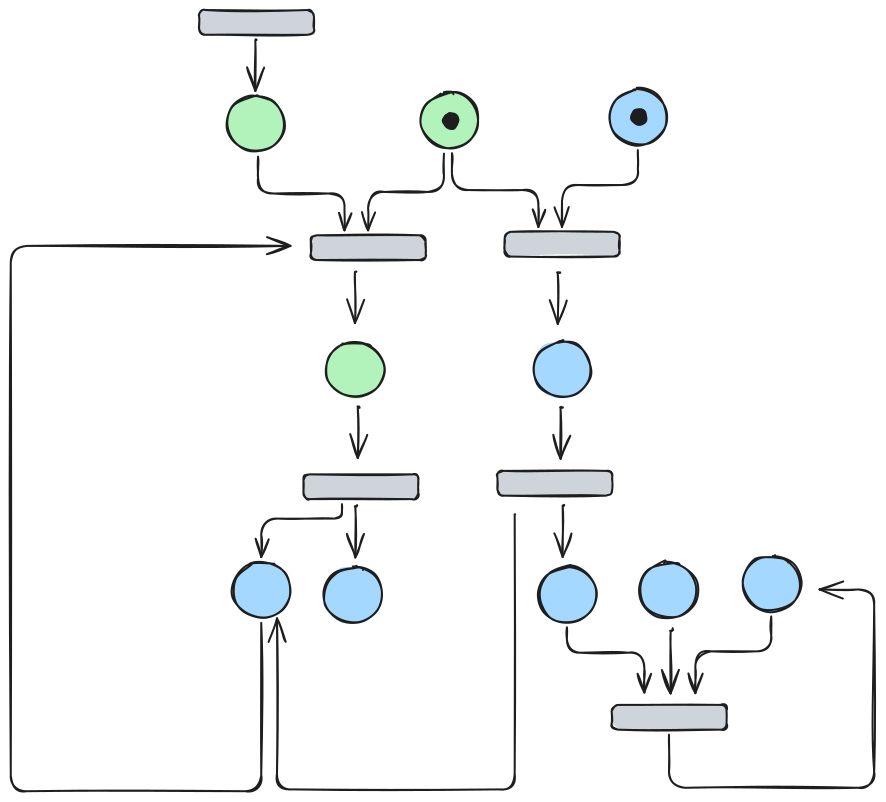
\includegraphics[width=\textwidth]{plots/bidirectional_pruning_step_a_updated.pdf}
%		\caption{Step 0: initial Petri net, before slicing.}
%		\label{fig:step:a}
%	\end{subfigure}\hfill
%	\begin{subfigure}[b]{0.45\textwidth}
%		\centering
%		\includegraphics[width=\textwidth]{plots/bidirectional_pruning_step_b_updated.pdf}
%		\caption{Step 1: first forward pass.}
%		\label{fig:step:b}
%	\end{subfigure}
%	
%	\vspace{1em}
%	
%	% Bottom row: (c), (d), and (e) matching (d)’s height
%	\begin{subfigure}[b]{0.30\textwidth}
%		\centering
%		\includegraphics[width=\textwidth]{plots/bidirectional_pruning_step_c_updated.pdf}
%		\caption{Step 2: first backward pass.}
%		\label{fig:step:c}
%	\end{subfigure}\hfill
%	\begin{subfigure}[b]{0.23\textwidth}
%		\centering
%		\includegraphics[width=\textwidth]{plots/bidirectional_pruning_step_d_updated_2.pdf}
%		\caption{Step 3: second forward pass.}
%		\label{fig:step:d}
%	\end{subfigure}\hfill
%	% <-- three-arg form: [vpos][total height][inner vpos]
%	\begin{subfigure}[b][\subfigheight][b]{0.23\textwidth}
%		\centering
%		\includegraphics[width=\textwidth]{plots/bidirectional_pruning_step_e_updated_2.pdf}
%		\caption{Step 4: final Petri net.}
%		\label{fig:step:e}
%	\end{subfigure}
%	
%	\caption{A Petri net during three rounds of bidirectional slicing: two forward passes and one backward pass. Black dots represent initial token markings; green places represent places that are allowed to be reachable in our constraints (i.e., aren't fixed to zero tokens in the final marking). Dashed shapes represent places and transitions that are identified as removable in the current iteration, and will be removed after it ends.}
%	\label{fig:bidirectional_pruning}
%\end{figure}

%\newpage

\clearpage

\section{Evaluation: Full Results}
\label{appendix:full_results}

See Table~\ref{tab:benchmarks-all}.
%\begin{table}[htbp]
%	\centering
%	% Load the tabular from the external file:
%	\begin{table}[H]
	\centering
	\begin{tabular}{l r r r r}
		\toprule
		& \multicolumn{2}{c}{Average time (ms)} 
		& \multicolumn{2}{c}{Median time (ms)} \\
		\cmidrule(lr){2-3} \cmidrule(lr){4-5}
		Category
		& \shortstack{certificate\\generation}
		& total
		& \shortstack{certificate\\generation}
		& total \\
		\midrule
		Serializable      &   2{,}273 &  25{,}531 &  1{,}178 &  2{,}238 \\
		Not serializable  &  42{,}076 &  42{,}980 &   773 &   830 \\
		All               &  39{,}613 &  52{,}858 &   797 &  2{,}080 \\
		\bottomrule
	\end{tabular}
\end{table}

%	\caption{Average and median runtime. Values are rounded to the nearest integer, to reduce clutter. The \textit{total} column also includes the time for validation.}
%	\label{tab:stats-summary}
%\end{table}


\todo{check table}
\begin{table}[h]
	\centering
	\small
	\setlength{\tabcolsep}{5pt}
	\renewcommand{\arraystretch}{0.9}
	
	\begin{tabular*}{\textwidth}{@{\extracolsep{\fill}}%
			p{1.5cm}   % Category
			p{1.0cm}   % Benchmark
			c          % Serializable
			c c c c c c % Features
			r r        % Cert, Total
		}
		\toprule
		\multicolumn{2}{c}{\textbf{Benchmark}}
		& \textbf{Serializable}
		& \multicolumn{6}{c}{\textbf{Features}}
		& \multicolumn{2}{c}{\textbf{Runtime (ms)}} \\
		\cmidrule(lr){1-2} \cmidrule(lr){3-3} \cmidrule(lr){4-9} \cmidrule(lr){10-11}
		&
		&
		& If & While & \texttt{?} & Arith & Yield & Multi-req
		& Cert. & Total \\
		\midrule
		
		% Core expressions
		\multirow{7}{=}{Core expressions} 
		& \texttt{a1.ser} & \greencmark &  & \cmark &  &  &       &   & 2 & 47 \\
		& \texttt{a2.ser} & \xmark &  &        &  &  & \cmark &   & 280 & 296 \\
		& \texttt{a3.ser} & \greencmark &  &        &  &  &       &   & 1 & 32 \\
		& \texttt{a4.ser} & \greencmark &  &        &  &  & \cmark & \cmark & 637 & 1{,}071 \\
		& \texttt{a5.ser} & \greencmark &  & \cmark &  &  & \cmark & \cmark & 3{,}234 & 13{,}624 \\
		& \texttt{a6.ser} & \xmark &  &        &  &  & \cmark & \cmark & 757 & 775 \\
		& \texttt{a7.ser} & \greencmark & \cmark & \cmark &  &  & \cmark &   & 4 & 33 \\
		\midrule
		
		% State machines
		\multirow{4}{=}{State machines} 
		& \texttt{b1.json} & \greencmark & \cmark &        &  &  & \cmark & \cmark & 683 & 968 \\
		& \texttt{b2.json} & \greencmark & \cmark &        &  &  & \cmark & \cmark & 2{,}063 & 7{,}802 \\
		& \texttt{b3.json} & \greencmark & \cmark &        &  &  & \cmark & \cmark & 730 & 2{,}080 \\
		& \texttt{b4.json} & \greencmark & \cmark &        &  &  & \cmark & \cmark & 660 & 1{,}909 \\
		\midrule
		
		% Mixed arithmetic
		\multirow{8}{=}{Mixed arithmetic} 
		& \texttt{c1.ser} & \xmark &  & \cmark &  & \cmark & \cmark & \cmark & 356{,}195 & 356{,}299 \\
		& \texttt{c2.ser} & \greencmark &  & \cmark &  & \cmark & \cmark & \cmark & 9{,}858 & 292{,}228 \\
		& \texttt{c3.ser} & \greencmark &  & \cmark &  & \cmark & \cmark & \cmark & 1{,}886 & 2{,}397 \\
		& \texttt{c4.ser} & \greencmark &  & \cmark &  & \cmark & \cmark & \cmark & 4{,}336 & 7{,}193 \\
		& \texttt{c5.ser} & \xmark &  & \cmark &  & \cmark & \cmark & \cmark & 43{,}694 & 43{,}735 \\
		& \texttt{c6.ser} & \xmark &  & \cmark &  & \cmark & \cmark & \cmark & 629 & 698 \\
		& \texttt{c7.ser} & \xmark &  & \cmark &  & \cmark & \cmark & \cmark & 797 & 875 \\
		& \texttt{c8.ser} & \greencmark &  & \cmark &  & \cmark & \cmark & \cmark & 4{,}357 & 8{,}931 \\
		\midrule
		
		% Circular increment
		\multirow{5}{=}{Circular increment} 
		& \texttt{d1.ser} & \greencmark & \cmark & \cmark & \cmark &  & \cmark &   & 2{,}391 & 5{,}373 \\
		& \texttt{d2.ser} & \xmark & \cmark &        & \cmark &  &   \cmark &   & 628 & 731 \\
		& \texttt{d3.ser} & \greencmark & \cmark & \cmark & \cmark &  &  \cmark &   & 2{,}642 & 10{,}266 \\
		& \texttt{d4.ser} & \greencmark & \cmark & \cmark & \cmark &  &     \cmark &   & 5{,}604 & 22{,}249 \\
		& \texttt{d5.ser} & \xmark & \cmark &        &  &  & \cmark &   & 495 & 554 \\
		\midrule
		
		% Concurrency & locking loops
		\multirow{7}{=}{Concurrency \& locking loops} 
		& \texttt{e1.ser} & \greencmark &  & \cmark &  &  & \cmark &   & 351 & 502 \\
		& \texttt{e2.ser} & \xmark & \cmark & \cmark &  & \cmark & \cmark & \cmark & \texttt{TIMEOUT} & \texttt{TIMEOUT} \\
		& \texttt{e3.ser} & \xmark & \cmark & \cmark &  & \cmark &   \cmark & \cmark & 24{,}899 & 25{,}039 \\
		& \texttt{e4.ser} & \xmark & \cmark & \cmark &  &  \cmark &   \cmark & \cmark & 273{,}062 & 273{,}351 \\
		& \texttt{e5.ser} & \greencmark & \cmark & \cmark & \cmark &  & \cmark &   & 2 & 55 \\
		& \texttt{e6.ser} & \greencmark & \cmark & \cmark & \cmark &  & \cmark &   & 10 & 114 \\
		& \texttt{e7.ser} & \greencmark &  & \cmark &  &  &   \cmark &   & 299 & 444 \\
		\midrule
		
		% Non-determinism
		\multirow{9}{=}{Non-determinism} 
		& \texttt{f1.ser} & \greencmark & \cmark &    \cmark    & \cmark &  & \cmark &   & 388 & 494 \\
		& \texttt{f2.ser} & \xmark & \cmark &   \cmark     & \cmark &  & \cmark &   & 612 & 676 \\
		& \texttt{f3.ser} & \xmark &  &        &  & \cmark &   \cmark & \cmark & 653 & 716 \\
		& \texttt{f4.ser} & \greencmark &  &     \cmark   &  & \cmark & \cmark & \cmark & 1{,}626 & 9{,}515 \\
		& \texttt{f5.ser} & \greencmark & \cmark &        & \cmark &  &       &   & 7{,}401 & 11{,}301 \\
		& \texttt{f6.ser} & \xmark & \cmark &        & \cmark &  & \cmark &   & 646 & 830 \\
		& \texttt{f7.ser} & \xmark & \cmark &        & \cmark &  &  \cmark &   & 400 & 427 \\
		& \texttt{f8.ser} & \xmark & \cmark &        & \cmark &  &   \cmark &   & 773 & 802 \\
		& \texttt{f9.ser} & \greencmark & \cmark &        & \cmark &  &  \cmark &   & 10 & 94 \\
		\midrule
		
		% Network & system protocols
		\multirow{7}{=}{Network \& system protocols} 
		& \texttt{g1.ser} & \xmark & \cmark & \cmark &  & \cmark & \cmark & \cmark & 59{,}312 & 74{,}539 \\
		& \texttt{g2.ser} & \greencmark & \cmark & \cmark &  & \cmark & \cmark & \cmark & \texttt{TIMEOUT} & \texttt{TIMEOUT} \\
		& \texttt{g3.ser} & \xmark & \cmark & \cmark & \cmark & \cmark & \cmark & \cmark & 20{,}557 & 20{,}954 \\
		& \texttt{g4.ser} & \xmark & \cmark & \cmark & \cmark & \cmark & \cmark & \cmark & 6{,}859 & 7{,}047 \\
		& \texttt{g5.ser} & \greencmark & \cmark & \cmark & \cmark & \cmark &   \cmark & \cmark & 3{,}047 & 12{,}324 \\
		& \texttt{g6.ser} & \xmark & \cmark &        & \cmark & \cmark & \cmark &   & 8{,}193 & 8{,}285 \\
		& \texttt{g7.ser} & \greencmark & \cmark &        & \cmark & \cmark &       &   & 6{,}886 & 252{,}752 \\
		\bottomrule
	\end{tabular*}
	
	\caption{Overview of our benchmarks and semilinear set reductions (timeouts: 500 ms).}
	\label{tab:benchmarks-all}
\end{table}



%\begin{table}[htbp]
%	\centering
%	% Load the tabular from the external file:
%	\begin{table}[H]
	\centering
	\small
	% increase horizontal padding between columns
	\setlength{\tabcolsep}{5pt}
	\renewcommand{\arraystretch}{0.9}
	\begin{tabular*}{\textwidth}{@{\extracolsep{\fill}}%
			p{1.5cm}   % Category
			p{1.0cm} % Benchmark
			c        % Serializable
			c c c c c c % Features
			r r       % Cert, Total
		}
		\toprule
		\multicolumn{2}{c}{\textbf{Benchmark}}
		& \textbf{Serializable}
		& \multicolumn{6}{c}{\textbf{Features}}
		& \multicolumn{2}{c}{\textbf{Runtime (ms)}} \\
		\cmidrule(lr){1-2} \cmidrule(lr){3-3} \cmidrule(lr){4-9} \cmidrule(lr){10-11}
		&
		&
		& If & While & \texttt{?} & Arith & Yield & Multi-req
		& Cert. & Total \\
		\midrule
		\multirow{7}{=}{Core expressions} & \texttt{a1.ser} & \greencmark &  & \cmark &  &  &       &   & 2 & 47 \\
		 & \texttt{a2.ser} & \xmark &  &        &  &  & \cmark &   & 280 & 296 \\
		 & \texttt{a3.ser} & \greencmark &  &        &  &  &       &   & 1 & 32 \\
		 & \texttt{a4.ser} & \greencmark &  &        &  &  & \cmark & \cmark & 637 & 1{,}071 \\
		 & \texttt{a5.ser} & \greencmark &  & \cmark &  &  & \cmark & \cmark & 3{,}234 & 13{,}624 \\
		 & \texttt{a6.ser} & \xmark &  &        &  &  & \cmark & \cmark & 757 & 775 \\
		 & \texttt{a7.ser} & \greencmark & \cmark & \cmark &  &  & \cmark &   & 4 & 33 \\
		\midrule
		\multirow{4}{=}{State machines} & \texttt{b1.json} & \greencmark & \cmark &        &  &  & \cmark & \cmark & 683 & 968 \\
		 & \texttt{b2.json} & \greencmark & \cmark &        &  &  & \cmark & \cmark & 2{,}063 & 7{,}802 \\
		 & \texttt{b3.json} & \greencmark & \cmark &        &  &  & \cmark & \cmark & 730 & 2{,}080 \\
		 & \texttt{b4.json} & \greencmark & \cmark &        &  &  & \cmark & \cmark & 660 & 1{,}909 \\
		\midrule
		\multirow{8}{=}{Mixed arithmetic} & \texttt{c1.ser} & \xmark &  & \cmark &  & \cmark & \cmark & \cmark & 356{,}195 & 356{,}299 \\
		 & \texttt{c2.ser} & \greencmark &  & \cmark &  & \cmark & \cmark & \cmark & 9{,}858 & 292{,}228 \\
		 & \texttt{c3.ser} & \greencmark &  & \cmark &  & \cmark & \cmark & \cmark & 1{,}886 & 2{,}397 \\
		 & \texttt{c4.ser} & \greencmark &  & \cmark &  & \cmark & \cmark & \cmark & 4{,}336 & 7{,}193 \\
		 & \texttt{c5.ser} & \xmark &  & \cmark &  & \cmark & \cmark & \cmark & 43{,}694 & 43{,}735 \\
		 & \texttt{c6.ser} & \xmark &  & \cmark &  & \cmark & \cmark & \cmark & 629 & 698 \\
		 & \texttt{c7.ser} & \xmark &  & \cmark &  & \cmark & \cmark & \cmark & 797 & 875 \\
		 & \texttt{c8.ser} & \greencmark &  & \cmark &  & \cmark & \cmark & \cmark & 4{,}357 & 8{,}931 \\
		\midrule
		\multirow{5}{=}{Circular increment} & \texttt{d1.ser} & \greencmark & \cmark & \cmark & \cmark &  & \cmark &   & 2{,}391 & 5{,}373 \\
		 & \texttt{d2.ser} & \xmark & \cmark &        & \cmark &  &   \cmark &   & 628 & 731 \\
		 & \texttt{d3.ser} & \greencmark & \cmark & \cmark & \cmark &  &  \cmark &   & 2{,}642 & 10{,}266 \\
		 & \texttt{d4.ser} & \greencmark & \cmark & \cmark & \cmark &  &     \cmark &   & 5{,}604 & 22{,}249 \\
		 & \texttt{d5.ser} & \xmark & \cmark &        &  &  & \cmark &   & 495 & 554 \\
		\midrule
		\multirow{7}{=}{Concurrency \& locking loops} & \texttt{e1.ser} & \greencmark &  & \cmark &  &  & \cmark &   & 351 & 502 \\
		 & \texttt{e2.ser} & \xmark & \cmark & \cmark &  & \cmark & \cmark & \cmark & \texttt{TIMEOUT} & \texttt{TIMEOUT} \\
		 & \texttt{e3.ser} & \xmark & \cmark & \cmark &  & \cmark &   \cmark & \cmark & 24{,}899 & 25{,}039 \\
		 & \texttt{e4.ser} & \xmark & \cmark & \cmark &  &  \cmark &   \cmark & \cmark & 273{,}062 & 273{,}351 \\
		 & \texttt{e5.ser} & \greencmark & \cmark & \cmark & \cmark &  & \cmark &   & 2 & 55 \\
		 & \texttt{e6.ser} & \greencmark & \cmark & \cmark & \cmark &  & \cmark &   & 10 & 114 \\
		 & \texttt{e7.ser} & \greencmark &  & \cmark &  &  &   \cmark &   & 299 & 444 \\
		\midrule
		\multirow{9}{=}{Non-deterministic \& randomness} & \texttt{f1.ser} & \greencmark & \cmark &    \cmark    & \cmark &  & \cmark &   & 388 & 494 \\
		 & \texttt{f2.ser} & \xmark & \cmark &   \cmark     & \cmark &  & \cmark &   & 612 & 676 \\
		 & \texttt{f3.ser} & \xmark &  &        &  & \cmark &   \cmark & \cmark & 653 & 716 \\
		 & \texttt{f4.ser} & \greencmark &  &     \cmark   &  & \cmark & \cmark & \cmark & 1{,}626 & 9{,}515 \\
		 & \texttt{f5.ser} & \greencmark & \cmark &        & \cmark &  &       &   & 7{,}401 & 11{,}301 \\
		 & \texttt{f6.ser} & \xmark & \cmark &        & \cmark &  & \cmark &   & 646 & 830 \\
		 & \texttt{f7.ser} & \xmark & \cmark &        & \cmark &  &  \cmark &   & 400 & 427 \\
		 & \texttt{f8.ser} & \xmark & \cmark &        & \cmark &  &   \cmark &   & 773 & 802 \\
		 & \texttt{f9.ser} & \greencmark & \cmark &        & \cmark &  &  \cmark &   & 10 & 94 \\
		\midrule
		\multirow{7}{=}{Networking \& system protocols} & \texttt{g1.ser} & \xmark & \cmark & \cmark &  & \cmark & \cmark & \cmark & 59{,}312 & 74{,}539 \\
		 & \texttt{g2.ser} & \greencmark & \cmark & \cmark &  & \cmark & \cmark & \cmark & \texttt{TIMEOUT} & \texttt{TIMEOUT} \\
		 & \texttt{g3.ser} & \xmark & \cmark & \cmark & \cmark & \cmark & \cmark & \cmark & 20{,}557 & 20{,}954 \\
		 & \texttt{g4.ser} & \xmark & \cmark & \cmark & \cmark & \cmark & \cmark & \cmark & 6{,}859 & 7{,}047 \\
		 & \texttt{g5.ser} & \greencmark & \cmark & \cmark & \cmark & \cmark &   \cmark & \cmark & 3{,}047 & 12{,}324 \\
		 & \texttt{g6.ser} & \xmark & \cmark &        & \cmark & \cmark & \cmark &   & 8{,}193 & 8{,}285 \\
		 & \texttt{g7.ser} & \greencmark & \cmark &        & \cmark & \cmark &       &   & 6{,}886 & 252{,}752 \\
		\midrule
\bottomrule
	\end{tabular*}
\end{table}

%	\caption{Overview of our benchmarks (\texttt{TIMEOUT} is $500$ seconds).}
%	\label{tab:benchmarks-all}
%\end{table}





\subsection{Optimization Analysis}
\label{subsec:optimization-results}

%Next of our four optimizations, and analyzed their effect on the overall runtime and space resources.
%
%All experiments were run with a \texttt{TIMEOUT} value of $150$ seconds.


\subsubsection{Runtime optimization.}

We ran all benchmarks with each of the following six optimization configurations: 
(i) without any optimization (marked [\texttt{\textbf{\text{-}\text{-}\text{-}\text{-}}}] in Fig.~\ref{fig:timeout_cumulative_solved_log}); (ii) with bidirectional slicing (marked [\texttt{\textbf{\text{B}\text{-}\text{-}\text{-}}}]); (iii) with redundant constraint elimination (marked [\texttt{\textbf{\text{-}\text{R}\text{-}\text{-}}}]); (iv) with generation of fewer constraints (marked [\texttt{\textbf{\text{-}\text{-}\text{G}\text{-}}}]);
(v) with strategic Kleene elimination (marked [\texttt{\textbf{\text{-}\text{-}\text{-}\text{S}}}]);
and finally, (vi) with all optimizations altogether (marked [\texttt{\textbf{\text{B}\text{R}\text{G}\text{S}}}]).
%
The results of the aggregated runtimes are presented in Fig.~\ref{fig:timeout_cumulative_solved_log} and show that over $28\%$ more benchmarks are solved when using all optimizations compared to running without any optimization.
%
Not surprisingly, the best configuration is the one with all optimizations on. 
%
Furthermore, the best single-optimization configurations with regard to runtime are [\texttt{\textbf{\text{-}\text{-}\text{G}\text{-}}}] and [\texttt{\textbf{\text{B}\text{-}\text{-}\text{-}}}], solving over $74\%$ and $72\%$ of the benchmarks respectively. 
%
We also note that the two remaining optimizations, [\texttt{\textbf{\text{-}\text{R}\text{-}\text{-}}}] and [\texttt{\textbf{\text{-}\text{-}\text{-}\text{S}}}], performed slightly worse (although not significantly) than without the optimizations when counting overall timeouts.
%
However, when analyzing the redundant constraint optimization (  [\texttt{\textbf{\text{-}\text{R}\text{-}\text{-}}}]), we identified instances in which it still \textit{strictly} improves runtime.
%
For example, the optimization affords a speedup of between $72.2\%$ and $85.2\%$ for benchmarks \texttt{a3.ser} and \texttt{a7.ser},  when compared to the baseline.

\subsubsection{Space optimization.}
Our optimizations also reduce the space complexity of the two main components --- the Petri net and the semilinear set.

\noindent
(1) \textbf{Petri net.} Bidirectional slicing (Fig.~\ref{fig:petri_size_reduction}) 
eliminates the average number of places \textit{by roughly half} --- from $23.91$ down to $12.79$. This optimization proved even more effective on transitions, \textit{eliminating about two-thirds}: from $37.3$ down to $12.61$. 
%Note that the pre-pruning averages were computed over $47$ nets (one per benchmark), whereas the post-pruning averages span $224$ nets, since each pre-pruning net gives rise to a separate pruned net per each disjunct.  
%\\

\noindent
(2) \textbf{Semilinear sets.} We ran an ablation experiment in which we compared all optimizations against runs where each of the three semilinear optimizations (i.e., all but PN slicing) was disabled. The redundant-constraint elimination (with a negated effect in [\texttt{\textbf{\text{B}\textcolor{red}{-}\text{G}\text{S}}}]) and the fewer-constraint generation elimination (with a negated effect in [\texttt{\textbf{\text{B}\text{R}\textcolor{red}{-}\text{S}}}]) \textit{drastically} reduced component counts, with the latter being especially effective in reducing the \textit{maximal} number of components to be up to $\mathbf{931\times}$ smaller, and the \textit{average} number of components to be up to $\mathbf{223\times}$ smaller (Table~\ref{tab:semilinear-size-reduction}), when compared to the baseline executions configured with all optimizations on ([\texttt{\textbf{\text{B}\text{R}\text{G}\text{S}}}]). 
%
For fairness, we measured only benchmarks completed under all configurations, excluding cases where semilinear sets exploded beyond $2^{30}$ components and timed out. Thus, our reported improvements actually \textit{understate} the true impact of these optimizations on memory. Such blowups, %especially common in state-machine benchmarks with NS loops, 
render even simple programs intractable without these optimizations.


%\subsubsection{Space Optimization}
%
%Our optimizations also reduce the space complexity of the two main components --- the Petri Net and the semilinear set.
%
%\smallskip
%\noindent
%\textbf{Petri Net size reduction.}
%%
%With all optimizations enabled, we evaluated (Fig.~\ref{fig:petri_size_reduction}) the impact of our bidirectional pruning by comparing, across all benchmarks, the average number of places and transitions removed due to this optimization. On average, pruning reduced the number of places \textit{by roughly half} --- dropping from $23.91$ places before pruning to $12.79$ places afterward. Pruning proved even more effective on transitions, \textit{eliminating about two-thirds} of them: from $37.3$ transitions on average before pruning down to $12.61$ afterward. Note that the pre-pruning averages were computed over $47$ nets (one per benchmark), whereas the post-pruning averages span $224$ nets, since each pre-pruning net gives rise to a separate pruned net per each disjunct. 
%of our reachability query. 
%These results are summarized in Fig.~\ref{fig:petri_size_reduction}.

%When running our tool with all optimizations on, we analyzed the effect of our bidirectional pruning, This was done be counting the average number of places and transitions before and after pruning, on all benchmarks.
%%
%The pruning resulted in a reduction of about half the number of original places --- from $23.91$ places on average \textit{before} pruning to $12.79$ places on average \textit{after} pruning.
%%
%The bidirectional was even more effective in reducing the transitions, as demonstrated by a removing about two thirds of the transitions --- resulting in pruned Petri Nets with $37.30$ transitions on average \textit{before} pruning to $12.61$ transitions on average \textit{after} pruning.
%%
%We note that the averaging for the pre-pruning step was done on $47$ nets, once per each benchmark, while the averaging for the post-pruning step was done on $224$ nets, as each pre-pruning net can give rise to multiple post-pruning nets, one per each disjunct in our reachability query.
%%
%These results are presented in Fig.~\ref{fig:petri_size_reduction}.


%Number of values for 'Before' bars:          47
%Number of values for 'After' bars:           224
%Average number of places before pruning:     23.91
%Average number of places after pruning:      12.79
%Average number of transitions before pruning: 37.30
%Average number of transitions after pruning:  12.61






%\smallskip
%\noindent
%\textbf{Semilinear set size reduction.}
%%
%Finally, our last experiment batch analyzed the size reduction among the semilinear sets.
%%
%Towards this end, we ran all our benchmarks with all optimizations to serve as a baseline. 
%%
%Then, we analyzed the effect of the three semilinear-related optimizations, i.e., all but the bidirectional pruning. For each of these three optimizations, we ran the benchmarks with all optimizations \textit{except} the one checked.
%%
%%Table~\ref{tab:semilinear-size-reduction} include a summary of the results, when comparing the semilinear set size.
%%
%Specifically, we compare both the average and the maximal (i) number of components; and (ii) period vectors per each component, as summarized in Table~\ref{tab:semilinear-size-reduction}.
%%
%The redundant constraint elimination and the generate-less-constraints optimizations had a highly significant effect on the number of components, with the latter being especially effective in reducing the maximal number of components to be $931$ times more compact, as well as the average number of components to be $223$ times more compact, when compared to the baseline.
%%
%To ensure a fair comparison, we only measured benchmarks that were completed under every configuration, deliberately excluding any case where the optimized semilinear set exploded beyond $2^{30}$ components and timed out. By excluding these intractable runs, our reported performance improvements actually \textit{understate} the true impact of these optimizations. This explosive growth and the resulting timeouts are especially pervasive among our state-machine benchmarks due to loops in their NS, rendering even simple programs infeasible without optimizations.
%
%In fact, for both these optimizations are even more effective as, in order to conduct a fair comparison, we analyzed only benchmarks that terminated in all combinations, an hence we do not include cases in which these two optimizations rendered the original semilinear set intractable, due to having over $2^{30}$ components (!), hence timing-out and being excluded from the analysis.
%%
%This occurs pervasively in our state-machine benchmarks which have loops in their network systems --- and hence even simple programs of this category cannot be analyzed with respect to serializability.

%\todo{understand why this is related to loops in the NS}

%
%\begin{center}
%	\begin{minipage}[htbp]{0.48\textwidth}
%		\centering
%		\includegraphics[width=\linewidth]{figures/cactus_plot.pdf}
%		\captionof{figure}{Solved instances (\texttt{TIMEOUT} $150$ s).}
%		\label{fig:timeout_cumulative_solved_log}
%	\end{minipage}\hfill
%	\begin{minipage}[htbp]{0.48\textwidth}
%		\centering
%		\includegraphics[width=\linewidth]{figures/petri_size_reduction_plot.pdf}
%		\captionof{figure}{PN size reduction via slicing.}
%		%(timeout 150 seconds)
%		%.}
%	\label{fig:petri_size_reduction}
%\end{minipage}
%\end{center}

%


\begin{figure}[h]
	\centering
	\includegraphics[width=0.68\linewidth]{figures/cactus_plot.pdf}
	\caption{Solved instances (\texttt{TIMEOUT} is 150 seconds).}
	\label{fig:timeout_cumulative_solved_log}
\end{figure}

%\begin{table}[!htbp]
%	\centering
%		\includegraphics[width=0.68\linewidth]{figures/cactus_plot.pdf}
%	\captionof{figure}{Solved instances (\texttt{TIMEOUT} is $150$ seconds).}
%	\label{fig:timeout_cumulative_solved_log}
%\end{table}


\begin{figure}[h]
	\centering
	\includegraphics[width=0.68\linewidth]{figures/petri_size_reduction_plot.pdf}
	\caption{PN size reduction via slicing.}
	\label{fig:petri_size_reduction}
\end{figure}



%\begin{table}[!htbp]
%	\centering
%	\includegraphics[width=0.68\linewidth]{figures/petri_size_reduction_plot.pdf}
%	\captionof{figure}{PN size reduction via slicing.}
%	%(timeout 150 seconds)
%	%.}
%	\label{fig:petri_size_reduction}
%\end{table}

%\begin{table}[!htbp]
%\centering
%\begin{minipage}[t]{0.48\linewidth}
%	\centering
%	\begin{table}[H]
	\centering
	\begin{tabular}{l r r r r}
		\toprule
		& \multicolumn{2}{c}{Average (ms)} 
		& \multicolumn{2}{c}{Median (ms)} \\
		\cmidrule(lr){2-3} \cmidrule(lr){4-5}
		Category
		& \shortstack{cert.}
		& total
		& \shortstack{cert.}
		& total \\
		\midrule
		\textcolor{ForestGreen}{Serializable}      &   2{,}273 &  25{,}531 &  1{,}178 &  2{,}238 \\
		\textcolor{red}{Not serializable}  &  42{,}076 &  42{,}980 &   773 &   830 \\
		All               &  39{,}613 &  52{,}858 &   797 &  2{,}080 \\
		\bottomrule
	\end{tabular}
\end{table}

%	\caption{Runtime for generated certificates (\texttt{total} also includes validation).}
%	%			Values are rounded to the nearest integer, to reduce clutter. 
%	%The \textit{total} column also includes the time for validation.}
%% NOTE - this excludes the 2 non-terminating runs (artifact also includes TIMEOUTs I think)
%\label{tab:stats-summary}
%\end{minipage}\hfill
%\begin{minipage}[t]{0.48\linewidth}
%\centering
%\begin{table}[H]
	\centering
	\begin{tabular}{l c c c c}
		\toprule
		& \multicolumn{2}{c}{components} & \multicolumn{2}{c}{periods/component} \\
		\cmidrule(lr){2-3} \cmidrule(lr){4-5}
		& average & max & average & max \\
		\midrule
	\texttt{\text{B}\text{R}\text{G}\text{S}} & 2.91 & 22 & 1.33 & 4 \\
	\texttt{\text{B}\textcolor{red}{-}\text{G}\text{S}} & 8.79 & 194 & \textbf{1.64} & 11 \\
	\texttt{\text{B}\text{R}\textcolor{red}{-}\text{S}} & \textbf{651.41} & \textbf{20{,}484} & 1.28 & \textbf{15} \\
	\texttt{\text{B}\text{R}\text{G}\textcolor{red}{-}} & 2.91 & 22 & 1.35 & 4 \\
  \bottomrule
	\end{tabular}
\end{table}

%\caption{Semilinear set size reduction via optimizations (baseline is [\texttt{\text{B}\text{R}\text{G}\text{S}}]).}
%\label{tab:semilinear-size-reduction}
%\end{minipage}
%\end{table}





%\begin{table}[!htbp]
%	\centering
%	\begin{table}[H]
	\centering
	\begin{tabular}{l c c c c}
		\toprule
		& \multicolumn{2}{c}{components} & \multicolumn{2}{c}{periods/component} \\
		\cmidrule(lr){2-3} \cmidrule(lr){4-5}
		& average & max & average & max \\
		\midrule
	\texttt{\text{B}\text{R}\text{G}\text{S}} & 2.91 & 22 & 1.33 & 4 \\
	\texttt{\text{B}\textcolor{red}{-}\text{G}\text{S}} & 8.79 & 194 & \textbf{1.64} & 11 \\
	\texttt{\text{B}\text{R}\textcolor{red}{-}\text{S}} & \textbf{651.41} & \textbf{20{,}484} & 1.28 & \textbf{15} \\
	\texttt{\text{B}\text{R}\text{G}\textcolor{red}{-}} & 2.91 & 22 & 1.35 & 4 \\
  \bottomrule
	\end{tabular}
\end{table}

%	\caption{Semilinear set size reduction via optimizations (baseline is [\texttt{\text{B}\text{R}\text{G}\text{S}}]).}
%	\label{tab:semilinear-size-reduction}
%\end{table}

\todo{check table}
%
\begin{table}[h]
	\centering
	\begin{tabular}{l c c c c}
		\toprule
		& \multicolumn{2}{c}{components} & \multicolumn{2}{c}{periods/component} \\
		\cmidrule(lr){2-3} \cmidrule(lr){4-5}
		& average & max & average & max \\
		\midrule
		\texttt{BRGS} & 2.91 & 22 & 1.33 & 4 \\
		\texttt{B}\textcolor{red}{-}\texttt{GS} & 8.79 & 194 & \textbf{1.64} & 11 \\
		\texttt{BR}\textcolor{red}{-}\texttt{S} & \textbf{651.41} & \textbf{20{,}484} & 1.28 & \textbf{15} \\
		\texttt{BRG}\textcolor{red}{-} & 2.91 & 22 & 1.35 & 4 \\
		\bottomrule
	\end{tabular}
	\caption{Semilinear set size reduction via optimizations (baseline is \texttt{BRGS}).}
	\label{tab:semilinear-size-reduction}
\end{table}




\section{Petri Net Model Checking}
\label{appendix:smpt}


%\smallskip
%\noindent
\subsection{Petri nets and VAS(S) reachability.}
%\label{sec:related:petri}
	
	Our work builds on both theoretical and practical advances in 
	Petri net research~\cite{Mu89, Es96, Re12, EsNi24}, and specifically, Petri net model checking.
	%The undecidability we prove 
	%for equivalence of interleavings stems from Hack’s seminal result~\cite{Ha76, 
		%HaThesis76} showing the undecidability of reachability set equivalence for 
	%Petri Nets. This undecidability originates in a series of reductions from 
	%Hilbert’s 10th problem, specifically the possibility of determining whether 
	%there exists an integer root for Diophantine equations, a problem that was 
	%later proven undecidable by Matijasēvič~\cite{Ma70}.
	%%
	%Jančar~\cite{Ja95} later provided an alternative proof to this undecidability 
	%result, by showing that Petri Nets can simulate universal (and thus 
	%undecidable) 2-counter Minsky machines~\cite{Mi67}. In addition, Jančar further 
	%strengthened the original result by proving that undecidability holds even for 
	%Petri nets with just five unbounded places.
	%
	%Furthermore, our approach also builds on 
	While the solution is 
	straightforward for bounded nets (through exhaustive enumeration), the unbounded case is highly nontrivial and was first solved by 
	Mayr~\cite{Ma81}, with subsequent improvements by Kosaraju~\cite{Ko82} and 
	Lambert~\cite{La92}. Recent work~\cite{CzWo22} has also established this 
	problem is \texttt{Ackermann}-complete.
	%
	These theoretical advances in Petri net reachability have given rise to a 
	plethora of practical tools, including \texttt{KReach}~\cite{DiLa20}, 
	\texttt{DICER}~\cite{XiZhLi21}, \texttt{MARCIE}~\cite{HeRoSc13}, and others. 
	%
	Our implementation leverages \texttt{SMPT}~\cite{AmDa23}, a state-of-the-art model checker that combines SMT-solving with structural invariants~\cite{AmBeDa21,AmDaHu22}.
%	 (see Appendix~\ref{appendix:smpt}). 
	%However,
	%other PN model checkers can be used as well.
	
	
\subsection{SMPT}


\texttt{SMPT} (\emph{Satisfiability Modulo Petri Nets}) is a tool incorporating a portfolio of symbolic model checking techniques --- including Bounded Model Checking (BMC)~\cite{BiCiClZh99}, state equation reasoning~\cite{Mu77}, $k$-induction~\cite{ShSiSt20}, Property Directed Reachability (PDR)~\cite{Br11,AmDaHu22}, and random state space exploration. It acts as a front-end to an SMT solver (\texttt{Z3}~\cite{DeBj08} in our setting), while also incorporating domain-specific knowledge from Petri net theory, such as invariants and structural properties. \texttt{SMPT} has participated in the last five editions of the \textit{Model Checking Contest} (MCC), an international competition for model-checking tools. In its most recent participation, it achieved a bronze medal and a $100\%$ confidence level score, indicating it never returned an incorrect verdict~\cite{mcc:2025}.

\texttt{SMPT} distinguishes itself from other tools in two ways that are particularly relevant to our setting and motivate its adoption. First, to the best of our knowledge, it is the only model checker for Petri nets that provides a proof of its verdict, regardless of the underlying verification technique. This means it either produces a witness trace when the property is reachable, or, more interestingly, a certificate of non-reachability~\cite{AmDaHu22} when the property is found to be unreachable.
%
The second distinguishing feature relates to our ongoing work on polyhedral reductions~\cite{AmBeDa21}, as elaborated in~\Cref{sec:discussion}.



%\newpage

\end{document}
